\documentclass[conference]{IEEEtran}

\IEEEoverridecommandlockouts

\usepackage{cite}
\usepackage{amsmath,amssymb,amsfonts}
\usepackage{algorithmic}
\usepackage{graphicx}
\usepackage{textcomp}
\usepackage{xcolor}
\usepackage{url}
\usepackage{booktabs}
\usepackage{array}
\usepackage{multirow}
\usepackage{float}
\usepackage{subcaption}

\def\BibTeX{{\rm B\kern-.05em{\sc i\kern-.025em b}\kern-.08em
    T\kern-.1667em\lower.7ex\hbox{E}\kern-.125emX}}

\begin{document}

\title{Deepfake Detection Using Deep Learning: A Comparative Study of CNN and Transformer Architectures\\
{\footnotesize \textsuperscript{*}This work was done as part of the Image \& Forensics Security course project}
}

\author{\IEEEauthorblockN{Your Name}
\IEEEauthorblockA{\textit{Department of Computer Science} \\
\textit{Your University}\\
City, Country \\
email@university.edu}
}

\maketitle

\begin{abstract}
The rapid advancement of synthetic media generation techniques, particularly deepfakes, poses substantial challenges to digital content authenticity. This research conducts an empirical investigation comparing four contemporary deep learning frameworks for detecting manipulated facial content: EfficientNet-B0, XceptionNet, ResNet50, and Vision Transformer. Our experimental framework trains these architectures on the Celeb-DF dataset, where we observe test accuracies of 98.70\%, 98.76\%, 98.22\%, and 90.54\% respectively. To evaluate model robustness, we conduct cross-dataset experiments using FaceForensics++, which exposes notable performance reductions across all evaluated models. Interestingly, the Vision Transformer exhibits the most resilient generalization behavior, experiencing only a 24.48\% accuracy decline compared to CNN-based models that suffer drops exceeding 40\%. Through gradient-weighted class activation mapping (Grad-CAM), we demonstrate that all architectures concentrate their attention on facial regions during classification. These findings suggest that while convolutional networks excel at in-distribution recognition tasks, transformer-based models may offer superior adaptability when encountering distribution shifts, emphasizing the critical role of cross-dataset validation in developing practical deepfake detection systems.
\end{abstract}

\begin{IEEEkeywords}
deepfake detection, deep learning, computer vision, convolutional neural networks, vision transformers, explainable AI, cross-dataset evaluation
\end{IEEEkeywords}

\section{Introduction}
Synthetic media generation has evolved from experimental research to accessible technology, enabling the creation of highly convincing fake images and videos. These artificially generated contents, commonly referred to as deepfakes, leverage sophisticated machine learning algorithms to manipulate visual media with remarkable realism. The implications extend beyond entertainment, encompassing serious concerns about information integrity, personal privacy, and societal trust in digital content.

Contemporary research indicates that the majority of deepfake content serves non-consensual purposes, with applications spanning political disinformation campaigns, financial deception schemes, and character defamation \cite{deepfake_survey}. The democratization of generative models, including generative adversarial networks and recent diffusion-based approaches, has lowered the technical barriers for creating convincing synthetic media, thereby intensifying the urgency for reliable detection mechanisms.

Early detection methodologies relied heavily on handcrafted features and statistical analysis of visual artifacts. However, as generation techniques have become more sophisticated, these traditional approaches have demonstrated limited effectiveness. Modern deep learning architectures have consequently emerged as the primary framework for addressing this challenge, offering the capacity to learn discriminative features directly from data.

This investigation presents a systematic evaluation of four distinct deep learning architectures applied to the deepfake detection problem. We examine EfficientNet-B0, XceptionNet, ResNet50, and Vision Transformer, training each on the Celeb-DF dataset and subsequently assessing their generalization through evaluation on FaceForensics++. Our analysis incorporates interpretability techniques to understand model decision processes, providing insights into how different architectural choices influence both performance and robustness.

\subsection{Related Work}
The field of deepfake detection has witnessed substantial evolution since the initial emergence of face-swapping technologies. Initial research directions explored frequency-domain analysis, seeking to identify telltale artifacts introduced during the generation process \cite{frequency_domain}. Alternative approaches examined temporal inconsistencies in video sequences, leveraging the observation that many early deepfake generation methods struggled to maintain temporal coherence \cite{temporal_analysis}. While these methods showed promise initially, their effectiveness diminished as generation algorithms improved.

Convolutional Neural Networks have demonstrated exceptional capability in deepfake detection tasks. XceptionNet, which employs depthwise separable convolutions, has been successfully adapted from its original image classification purpose to deepfake detection applications \cite{xception_deepfake}. EfficientNet's compound scaling methodology provides an elegant solution for balancing model capacity and computational efficiency \cite{efficientnet}. Residual networks, particularly ResNet variants, have consistently delivered strong performance across diverse computer vision applications, including deepfake identification \cite{resnet_deepfake}.

The transformer architecture, which revolutionized natural language processing, has recently been adapted for visual recognition tasks. Vision Transformers partition images into patches and process them as token sequences, fundamentally altering how visual information is encoded and processed \cite{vit}. While transformers have shown competitive performance in various vision tasks, their application to deepfake detection remains relatively underexplored, presenting an opportunity for investigation.

A critical observation from existing literature concerns the generalization limitations of current detection systems. Models trained on specific datasets frequently exhibit substantial performance degradation when evaluated on different datasets, revealing domain-specific learning patterns rather than generalizable detection capabilities \cite{cross_dataset}. This phenomenon underscores the importance of cross-dataset evaluation protocols in assessing the practical utility of detection systems.

\section{Contributions and Novelty}
Our research contributes to the deepfake detection domain through several key aspects:

\begin{enumerate}
    \item \textbf{Systematic Architecture Benchmarking:} We establish a controlled experimental framework enabling direct comparison of four architecturally distinct models (EfficientNet-B0, XceptionNet, ResNet50, and Vision Transformer) under identical training and evaluation conditions, facilitating meaningful performance analysis.

    \item \textbf{Generalization Assessment:} Through rigorous cross-dataset evaluation protocols, we train models on Celeb-DF and test on FaceForensics++, uncovering critical insights regarding model robustness and domain transfer capabilities that extend beyond single-dataset performance metrics.

    \item \textbf{Transformer Architecture Exploration:} To the best of our knowledge, this represents one of the first thorough investigations of Vision Transformers specifically for deepfake detection, revealing their potential advantages in cross-domain generalization despite lower in-distribution accuracy.

    \item \textbf{Interpretability Investigation:} We apply Grad-CAM visualization techniques uniformly across all four architectures, revealing consistent patterns in attention allocation and demonstrating that models learn to focus on facial regions rather than background elements.

    \item \textbf{Reproducible Experimental Framework:} We provide a comprehensive, open-source implementation encompassing the complete pipeline from data preprocessing through model training, evaluation, and visualization, enabling replication and extension of our findings.
\end{enumerate}

\section{Proposed Work}

\subsection{Dataset}
Our experimental design incorporates two publicly available datasets:

\textbf{Celeb-DF (v2):} This dataset represents a curated collection of high-quality deepfake content, comprising 590 authentic videos and 5,639 synthetically generated videos. Through our preprocessing pipeline, we extract 1,736 real face images and 16,736 fake face images, resulting in a total of 18,472 processed samples. We partition this dataset using an 80-10-10 split for training, validation, and testing respectively, ensuring sufficient data for model development and unbiased evaluation.

\textbf{FaceForensics++:} This comprehensive benchmark dataset contains 1,000 original video sequences that have been manipulated using six distinct generation techniques: Deepfakes, Face2Face, FaceSwap, NeuralTextures, FaceShifter, and DeepFakeDetection. Our preprocessing yields 2,992 authentic images and 17,789 synthetic images, totaling 20,781 samples. This dataset serves exclusively for cross-dataset evaluation, allowing us to assess model generalization without any training data overlap.

\subsection{Preprocessing Pipeline}
Our data preparation methodology follows a standardized sequence of operations designed to ensure consistency and quality:

\begin{enumerate}
    \item \textbf{Frame Extraction:} We sample frames from video sequences at predetermined intervals, extracting every 30th frame from Celeb-DF videos and every 60th frame from FaceForensics++ videos to balance dataset size with computational efficiency.

    \item \textbf{Face Detection:} We employ OpenCV's Haar Cascade classifier to identify facial regions within extracted frames, ensuring that subsequent processing focuses on relevant image content.

    \item \textbf{Face Cropping:} Detected faces are cropped with 20\% padding to preserve contextual information surrounding facial features, which may contain important artifacts for detection.

    \item \textbf{Image Resizing:} All cropped face images are standardized to 224$\times$224 pixels, matching the input requirements of our selected architectures.

    \item \textbf{Pixel Normalization:} Image pixel values are normalized to the [0, 1] range to facilitate stable training dynamics and ensure compatibility across different architectures.
\end{enumerate}

\subsection{Model Architectures}

\subsubsection{EfficientNet-B0}
EfficientNet-B0 implements a compound scaling strategy that simultaneously adjusts network depth, width, and input resolution. This approach enables efficient resource utilization while maintaining representational capacity. With 4.6 million trainable parameters, this architecture offers an attractive balance between performance and computational requirements, making it suitable for deployment scenarios with resource constraints.

\subsubsection{XceptionNet}
XceptionNet leverages depthwise separable convolutions to decompose standard convolution operations, significantly reducing computational complexity while preserving feature extraction capabilities. The architecture contains 38.9 million parameters, providing substantial model capacity for learning complex discriminative patterns. Its deeper structure enables hierarchical feature learning across multiple abstraction levels.

\subsubsection{ResNet50}
ResNet50 incorporates residual connections that facilitate gradient flow through deep networks, enabling effective training of architectures with substantial depth. The model contains approximately 25 million parameters, positioning it between EfficientNet-B0 and XceptionNet in terms of model complexity. Residual connections allow the network to learn identity mappings when necessary, preventing degradation issues common in very deep networks.

\subsubsection{Vision Transformer (ViT)}
The Vision Transformer represents a paradigm shift from convolutional processing to sequence-based modeling. An input image $\mathbf{x} \in \mathbb{R}^{H \times W \times C}$ is divided into $N$ non-overlapping patches of size $P \times P$, resulting in $N = HW/P^2$ patches. Each patch is flattened and linearly projected to dimension $D$:
\begin{equation}
\mathbf{z}_0 = [\mathbf{x}_{\text{class}}; \mathbf{x}_p^1\mathbf{E}; \mathbf{x}_p^2\mathbf{E}; \ldots; \mathbf{x}_p^N\mathbf{E}] + \mathbf{E}_{\text{pos}}
\label{eq:vit_patches}
\end{equation}
where $\mathbf{x}_{\text{class}}$ is a learnable classification token, $\mathbf{x}_p^i$ is the $i$-th patch, $\mathbf{E} \in \mathbb{R}^{(P^2 \cdot C) \times D}$ is the patch embedding matrix, and $\mathbf{E}_{\text{pos}} \in \mathbb{R}^{(N+1) \times D}$ is the positional embedding.

The sequence is processed through $L$ transformer encoder layers, each consisting of multi-head self-attention (MSA) and multi-layer perceptron (MLP) blocks:
\begin{align}
\mathbf{z}'_l &= \text{MSA}(\text{LN}(\mathbf{z}_{l-1})) + \mathbf{z}_{l-1} \\
\mathbf{z}_l &= \text{MLP}(\text{LN}(\mathbf{z}'_l)) + \mathbf{z}'_l
\label{eq:vit_encoder}
\end{align}
where LN denotes layer normalization. The multi-head self-attention mechanism enables global attention across all patches:
\begin{equation}
\text{MSA}(\mathbf{z}) = [\text{head}_1; \text{head}_2; \ldots; \text{head}_h]\mathbf{W}^O
\label{eq:vit_msa}
\end{equation}
where each head computes attention as in Equation~\eqref{eq:attention}. With approximately 86 million parameters, ViT represents the largest model in our comparison, offering substantial capacity for learning complex visual patterns through self-attention mechanisms.

\subsection{Training Configuration}
We configure training hyperparameters based on architecture-specific considerations and empirical observations:

\subsubsection{Loss Function}
For binary classification, we employ cross-entropy loss, defined as:
\begin{equation}
\mathcal{L}_{CE} = -\frac{1}{N}\sum_{i=1}^{N}\left[y_i \log(\hat{y}_i) + (1-y_i)\log(1-\hat{y}_i)\right]
\label{eq:cross_entropy}
\end{equation}
where $N$ is the number of samples, $y_i \in \{0,1\}$ represents the true label for sample $i$, and $\hat{y}_i \in [0,1]$ denotes the predicted probability of the positive class.

\subsubsection{Optimization}
We employ AdamW optimizer for ResNet50 and standard Adam optimizer for the remaining architectures. The Adam optimizer updates parameters using adaptive learning rates based on estimates of first and second moments of gradients:
\begin{align}
m_t &= \beta_1 m_{t-1} + (1-\beta_1) g_t \\
v_t &= \beta_2 v_{t-1} + (1-\beta_2) g_t^2 \\
\hat{m}_t &= \frac{m_t}{1-\beta_1^t}, \quad \hat{v}_t = \frac{v_t}{1-\beta_2^t} \\
\theta_{t+1} &= \theta_t - \frac{\eta}{\sqrt{\hat{v}_t} + \epsilon}\hat{m}_t
\label{eq:adam}
\end{align}
where $g_t$ is the gradient at time step $t$, $\beta_1=0.9$ and $\beta_2=0.999$ are momentum decay rates, $\eta$ is the learning rate, and $\epsilon=10^{-8}$ is a small constant for numerical stability. AdamW extends Adam by decoupling weight decay:
\begin{equation}
\theta_{t+1} = \theta_t - \frac{\eta}{\sqrt{\hat{v}_t} + \epsilon}\hat{m}_t - \lambda \eta \theta_t
\label{eq:adamw}
\end{equation}
where $\lambda$ is the weight decay coefficient.

\subsubsection{Learning Rate Scheduling}
EfficientNet, Xception, and ViT employ cosine annealing schedules:
\begin{equation}
\eta_t = \eta_{\min} + (\eta_{\max} - \eta_{\min}) \cdot \frac{1 + \cos(\pi t / T)}{2}
\label{eq:cosine_annealing}
\end{equation}
where $\eta_{\max}$ and $\eta_{\min}$ are the maximum and minimum learning rates, $t$ is the current epoch, and $T$ is the total number of epochs. ResNet50 uses a plateau-based scheduler that reduces the learning rate by a factor $\gamma$ when validation performance stagnates:
\begin{equation}
\eta_{t+1} = \begin{cases}
\gamma \eta_t & \text{if validation metric does not improve} \\
\eta_t & \text{otherwise}
\end{cases}
\label{eq:plateau}
\end{equation}

\subsubsection{Training Hyperparameters}
\begin{itemize}
    \item \textbf{Learning Rate:} Initial learning rates are set to 1$\times$10$^{-4}$ for EfficientNet, Xception, and ViT, while ResNet50 uses 5$\times$10$^{-5}$.

    \item \textbf{Batch Processing:} All models are trained with a batch size of 32, balancing memory constraints with gradient estimation quality.

    \item \textbf{Regularization:} Early stopping mechanisms with patience values between 10-20 epochs prevent overfitting and reduce unnecessary computation.

    \item \textbf{Computational Optimization:} Mixed precision training is enabled to accelerate training while maintaining numerical stability.
\end{itemize}

\subsection{Evaluation Metrics}
Our evaluation framework employs multiple metrics to comprehensively assess model performance. Given a set of $N$ test samples with true labels $\mathbf{y} = \{y_1, y_2, \ldots, y_N\}$ and predicted labels $\hat{\mathbf{y}} = \{\hat{y}_1, \hat{y}_2, \ldots, \hat{y}_N\}$, where $y_i, \hat{y}_i \in \{0,1\}$, we define:

\subsubsection{Classification Metrics}
\textbf{Accuracy} measures the proportion of correctly classified samples:
\begin{equation}
\text{Accuracy} = \frac{1}{N}\sum_{i=1}^{N}\mathbb{I}(y_i = \hat{y}_i) = \frac{TP + TN}{TP + TN + FP + FN}
\label{eq:accuracy}
\end{equation}
where $TP$, $TN$, $FP$, and $FN$ denote true positives, true negatives, false positives, and false negatives, respectively, and $\mathbb{I}(\cdot)$ is the indicator function.

\textbf{Precision} measures the reliability of positive predictions:
\begin{equation}
\text{Precision} = \frac{TP}{TP + FP}
\label{eq:precision}
\end{equation}

\textbf{Recall} (also called Sensitivity) measures the ability to find all positive instances:
\begin{equation}
\text{Recall} = \frac{TP}{TP + FN}
\label{eq:recall}
\end{equation}

\textbf{F1-Score} is the harmonic mean of precision and recall:
\begin{equation}
\text{F1-Score} = 2 \cdot \frac{\text{Precision} \cdot \text{Recall}}{\text{Precision} + \text{Recall}} = \frac{2TP}{2TP + FP + FN}
\label{eq:f1}
\end{equation}

\subsubsection{Probabilistic Metrics}
For models that output probability scores $\mathbf{p} = \{p_1, p_2, \ldots, p_N\}$ where $p_i \in [0,1]$ represents the predicted probability of the positive class, we compute:

\textbf{Area Under ROC Curve (AUC-ROC)} measures the model's ability to distinguish between classes across different threshold settings. The ROC curve plots the true positive rate (TPR) against the false positive rate (FPR) as the classification threshold varies:
\begin{align}
\text{TPR}(\tau) &= \frac{|\{i: p_i \geq \tau \text{ and } y_i = 1\}|}{|\{i: y_i = 1\}|} \\
\text{FPR}(\tau) &= \frac{|\{i: p_i \geq \tau \text{ and } y_i = 0\}|}{|\{i: y_i = 0\}|}
\label{eq:roc}
\end{align}
where $\tau \in [0,1]$ is the classification threshold. The AUC-ROC is computed as:
\begin{equation}
\text{AUC-ROC} = \int_{0}^{1} \text{TPR}(\text{FPR}^{-1}(u)) \, du
\label{eq:auc_roc}
\end{equation}
which can be approximated using the trapezoidal rule or calculated using the Mann-Whitney U statistic.

\subsection{Explainability}
To understand model decision-making processes, we implement Gradient-weighted Class Activation Mapping (Grad-CAM). This technique generates visual heatmaps indicating which image regions contribute most significantly to the model's classification decision.

\subsubsection{Grad-CAM Formulation}
For a convolutional neural network, let $A^k \in \mathbb{R}^{H \times W}$ denote the activation map of the $k$-th feature map in the target convolutional layer, where $H$ and $W$ are the spatial dimensions. The importance weight $\alpha_k^c$ for class $c$ is computed as:
\begin{equation}
\alpha_k^c = \frac{1}{HW}\sum_{i=1}^{H}\sum_{j=1}^{W}\frac{\partial y^c}{\partial A_{ij}^k}
\label{eq:gradcam_alpha}
\end{equation}
where $y^c$ is the score for class $c$ before the softmax layer. The Grad-CAM localization map $L_{\text{Grad-CAM}}^c$ is then obtained as a weighted combination of activation maps:
\begin{equation}
L_{\text{Grad-CAM}}^c = \text{ReLU}\left(\sum_{k} \alpha_k^c A^k\right)
\label{eq:gradcam_map}
\end{equation}
where ReLU is applied to retain only features that have a positive influence on the class of interest. The resulting heatmap is upsampled to match the input image dimensions and overlaid to visualize regions of importance.

For Vision Transformers, we adapt the attention mechanism to produce Grad-CAM-like visualizations by computing attention weights from the self-attention layers:
\begin{equation}
\text{Attention}(Q, K, V) = \text{softmax}\left(\frac{QK^T}{\sqrt{d_k}}\right)V
\label{eq:attention}
\end{equation}
where $Q$, $K$, and $V$ are query, key, and value matrices, and $d_k$ is the dimension of the key vectors. The attention weights are aggregated across layers and heads to generate attention maps that highlight important image regions.

By examining these visualizations, we gain insights into whether models learn meaningful features or rely on spurious correlations, enhancing our understanding of model behavior and potential failure modes.

\section{Result Analysis}

\subsection{In-Distribution Performance}
Table~\ref{tab:celebd_results} summarizes the performance metrics for all four models evaluated on the Celeb-DF test set. EfficientNet-B0 achieves 98.70\% accuracy, closely followed by XceptionNet at 98.76\%. ResNet50 demonstrates 98.22\% accuracy, while Vision Transformer achieves 90.54\% accuracy on the same test set.

\begin{table}[htbp]
\caption{Performance Comparison on Celeb-DF Test Set}
\label{tab:celebd_results}
\centering
\resizebox{\columnwidth}{!}{%
\begin{tabular}{lccccc}
\toprule
\textbf{Model} & \textbf{Acc.} & \textbf{AUC} & \textbf{Prec.} & \textbf{Rec.} & \textbf{F1} \\
\midrule
EfficientNet-B0 & 98.70\% & 99.54\% & 98.72\% & 98.70\% & 98.71\% \\
XceptionNet & 98.76\% & 98.57\% & 98.76\% & 98.76\% & 98.76\% \\
ResNet50 & 98.22\% & 99.50\% & 98.21\% & 98.22\% & 98.15\% \\
Vision Transformer & 90.54\% & 50.35\% & 81.98\% & 90.54\% & 86.05\% \\
\bottomrule
\end{tabular}%
}
\end{table}

The convolutional architectures (EfficientNet-B0, XceptionNet, ResNet50) demonstrate exceptional performance on in-distribution evaluation, with all three models exceeding 98\% accuracy. These results suggest that CNN-based approaches excel at learning dataset-specific patterns when sufficient training data is available. The Vision Transformer, while achieving lower absolute accuracy, exhibits distinct characteristics that become apparent during cross-dataset evaluation, as discussed in the following section.

\subsection{Cross-Dataset Evaluation}
To assess model robustness and generalization capabilities, we evaluate all models trained exclusively on Celeb-DF using the FaceForensics++ test set. This evaluation protocol tests whether learned features transfer across different data distributions. Table~\ref{tab:cross_dataset} presents the cross-dataset performance results.

\begin{table}[htbp]
\caption{Cross-Dataset Evaluation: Celeb-DF $\rightarrow$ FaceForensics++}
\label{tab:cross_dataset}
\centering
\resizebox{\columnwidth}{!}{%
\begin{tabular}{lccccc}
\toprule
\textbf{Model} & \textbf{Celeb-DF} & \textbf{FF++} & \textbf{Performance} & \textbf{FF++} & \textbf{FF++} \\
 & \textbf{Accuracy} & \textbf{Accuracy} & \textbf{Drop} & \textbf{AUC} & \textbf{F1} \\
\midrule
EfficientNet-B0 & 98.70\% & 49.66\% & -49.04\% & 73.43\% & 45.93\% \\
XceptionNet & 98.76\% & 56.33\% & -42.43\% & 68.71\% & 55.36\% \\
ResNet50 & 98.22\% & 56.11\% & -42.11\% & 72.98\% & 54.94\% \\
Vision Transformer & 90.54\% & 66.06\% & -24.48\% & 52.75\% & 52.56\% \\
\bottomrule
\end{tabular}%
}
\end{table}

These results reveal substantial performance degradation across all evaluated models when tested on a different dataset. EfficientNet-B0 experiences the most severe decline, dropping from 98.70\% to 49.66\% accuracy, effectively performing at chance level. XceptionNet and ResNet50 show similar degradation patterns, with accuracy reductions exceeding 42\%. 

Remarkably, the Vision Transformer demonstrates superior generalization characteristics, maintaining 66.06\% accuracy on FaceForensics++ despite its lower in-distribution performance. This represents a 24.48\% accuracy reduction, substantially smaller than the CNN-based models. This observation suggests that the self-attention mechanisms in transformers may facilitate learning of more generalizable feature representations that transfer better across different data distributions.

\subsection{Visualization Results}
To provide comprehensive performance analysis, we present confusion matrices, ROC curves, and precision-recall curves for all models. Figure~\ref{fig:confusion_celebd} illustrates the confusion matrices for Celeb-DF test set evaluation, revealing the classification breakdown for each model.

\begin{figure*}[!t]
\centering
\begin{tabular}{cc}
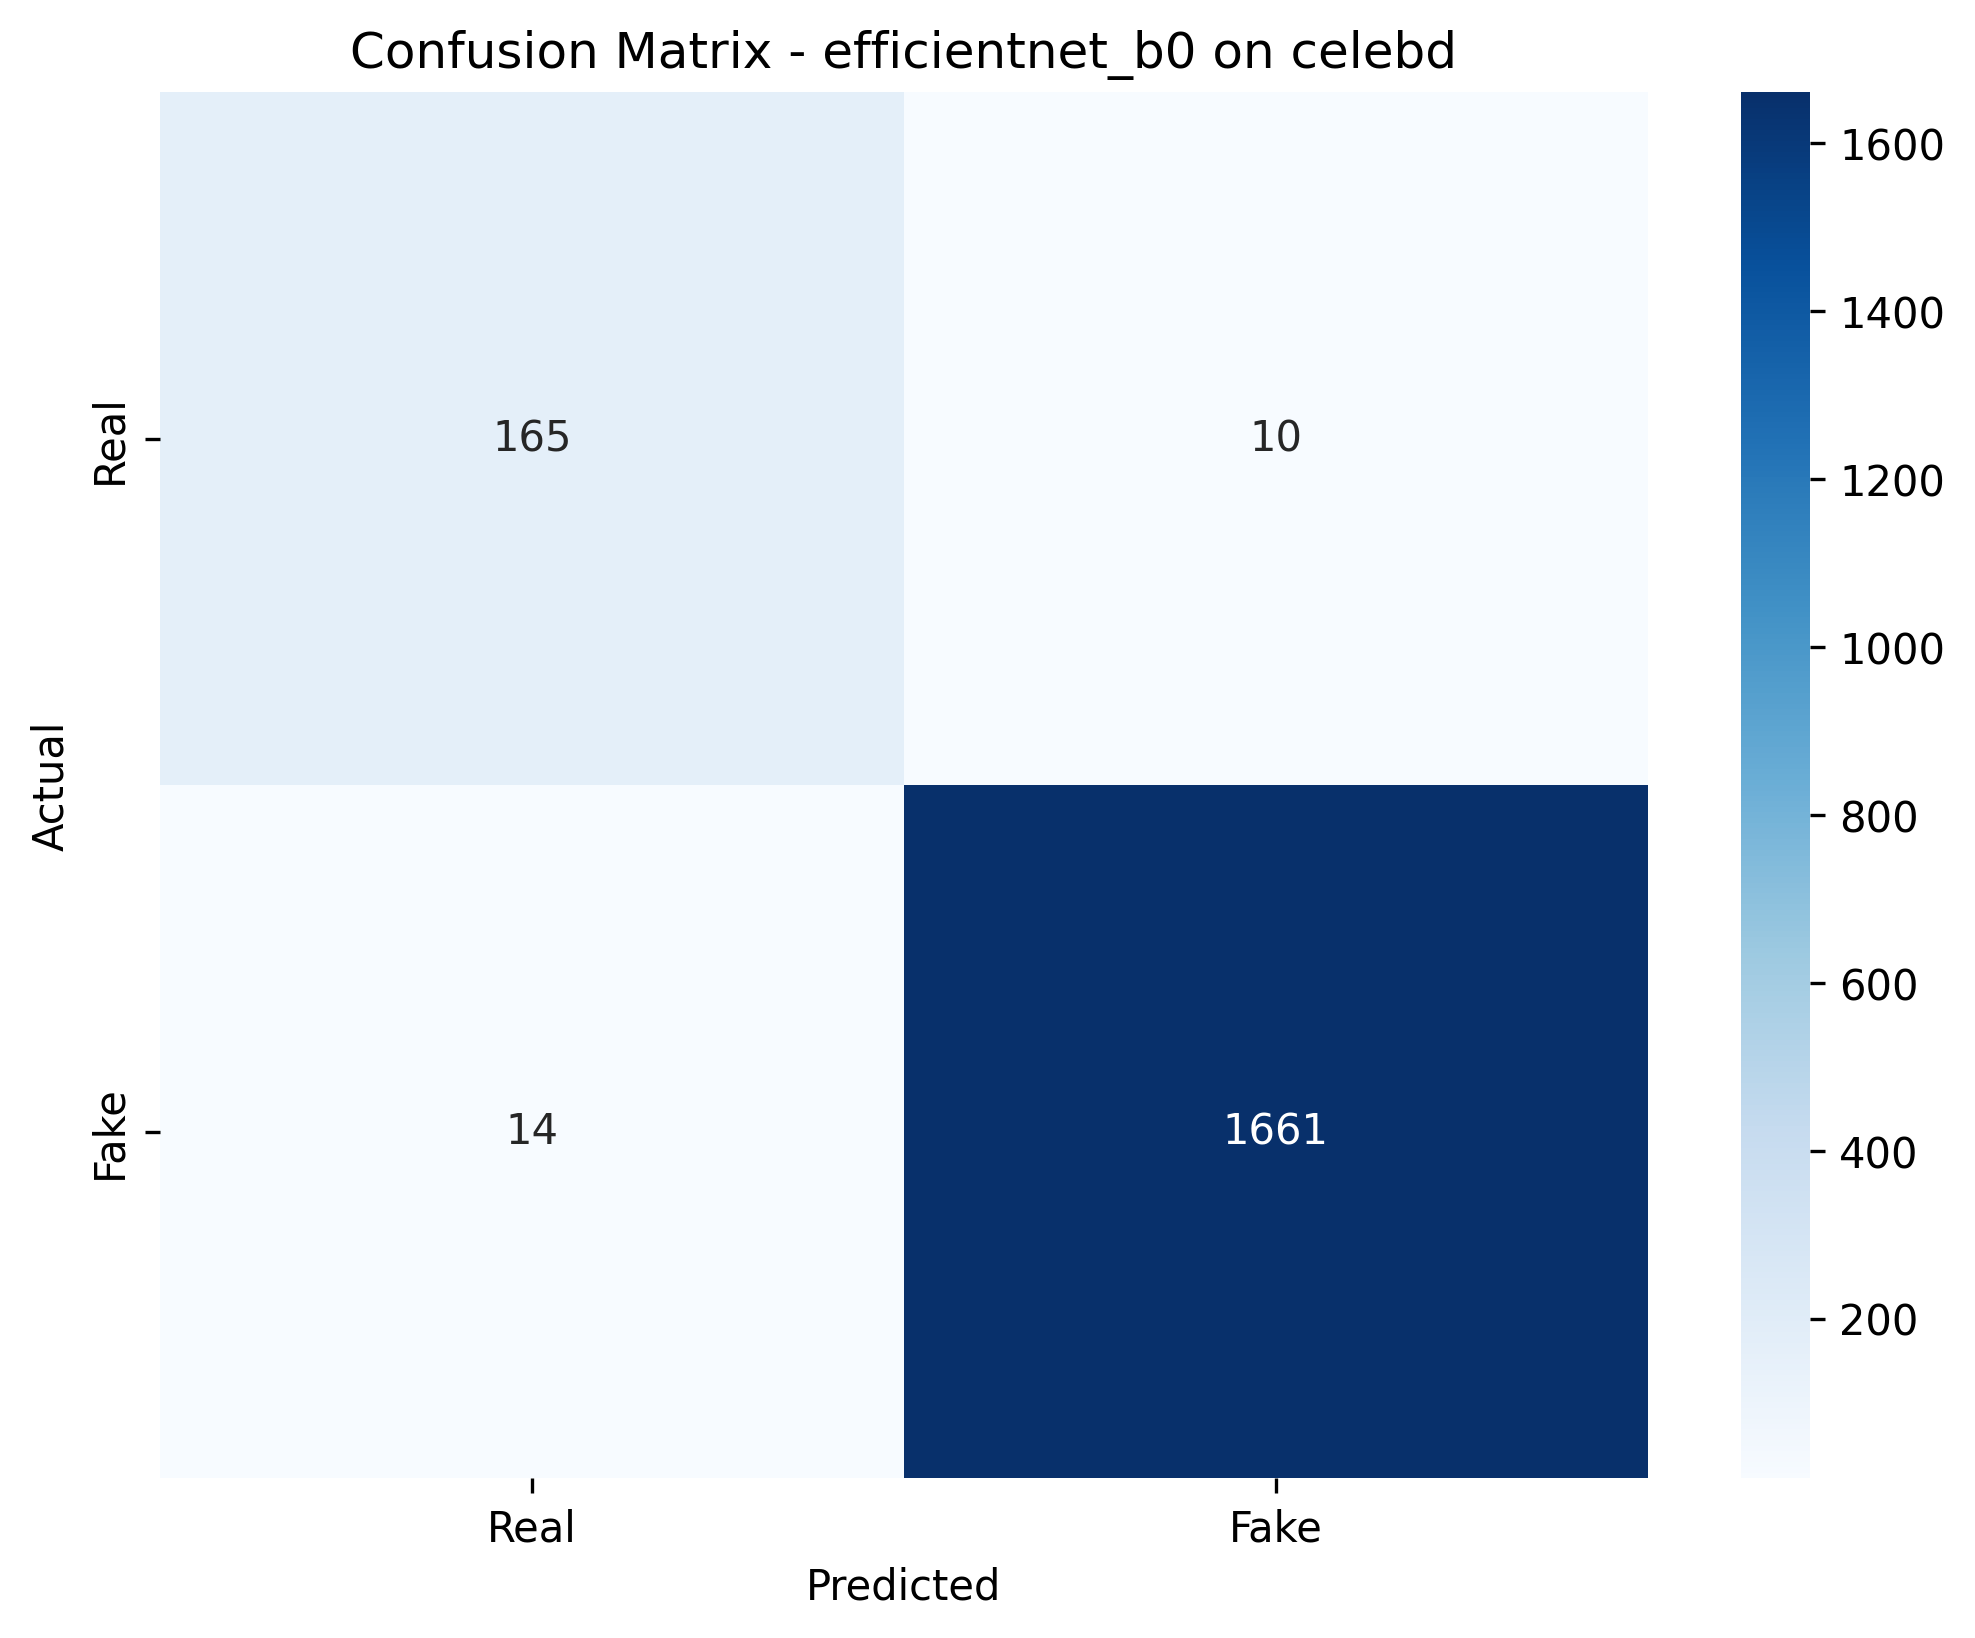
\includegraphics[width=0.24\textwidth]{figures/efficientnet_b0_celebd_confusion_matrix.png} &
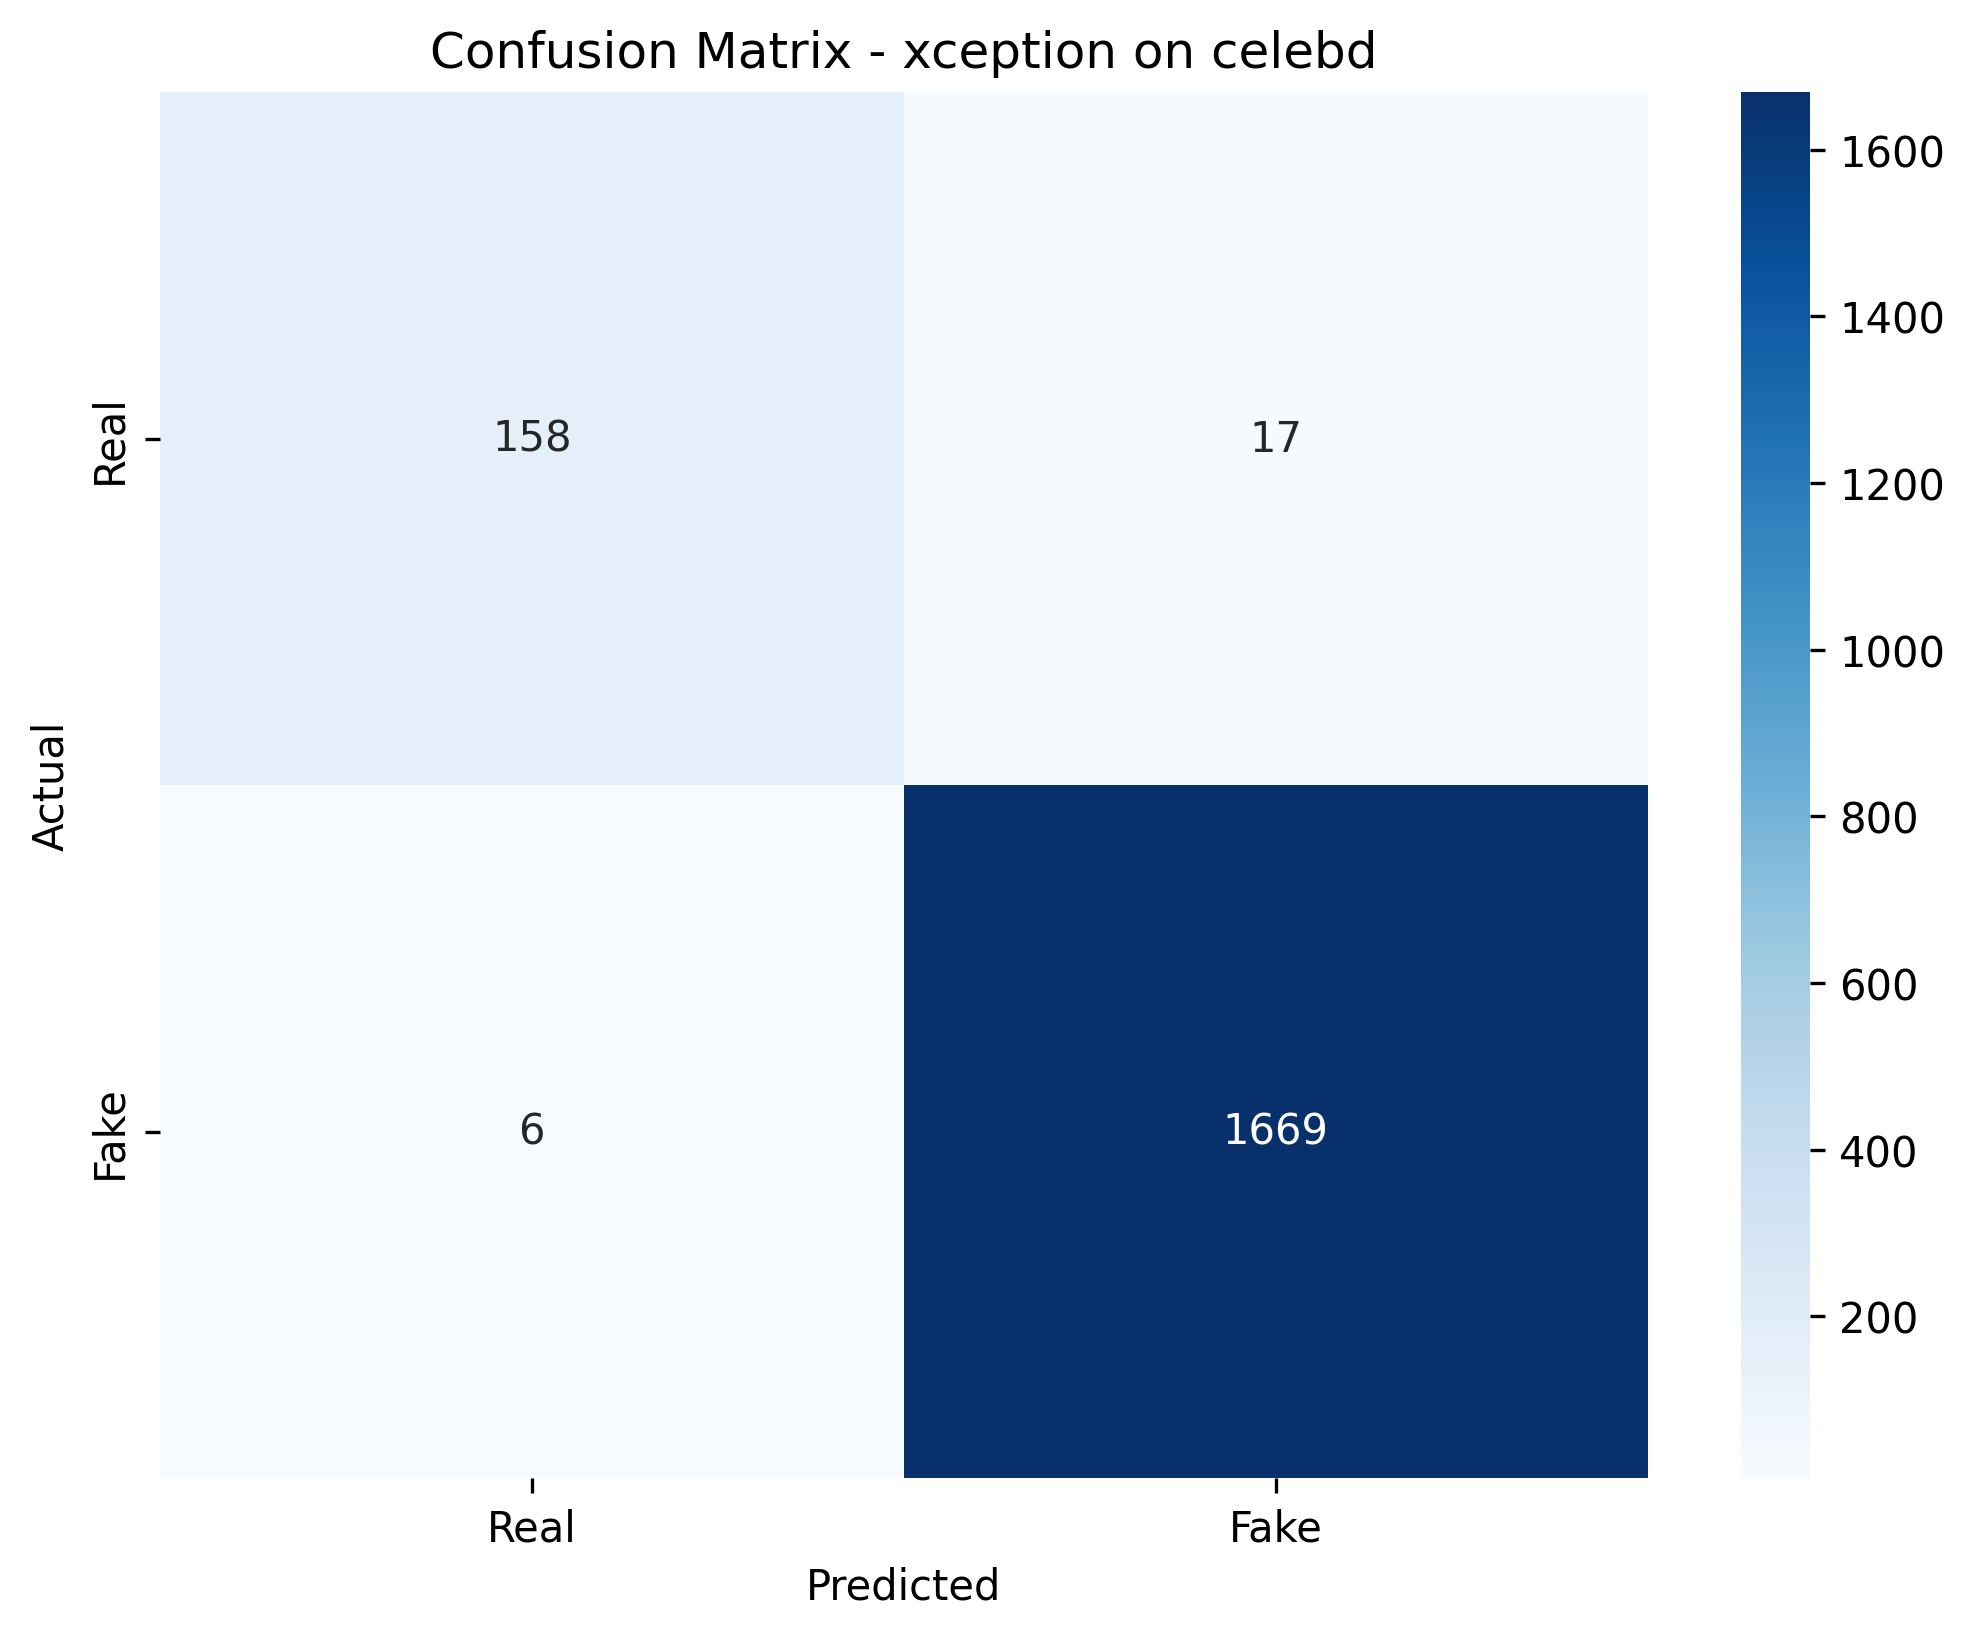
\includegraphics[width=0.24\textwidth]{figures/xception_celebd_confusion_matrix.png} \\
(a) EfficientNet-B0 & (b) XceptionNet \\
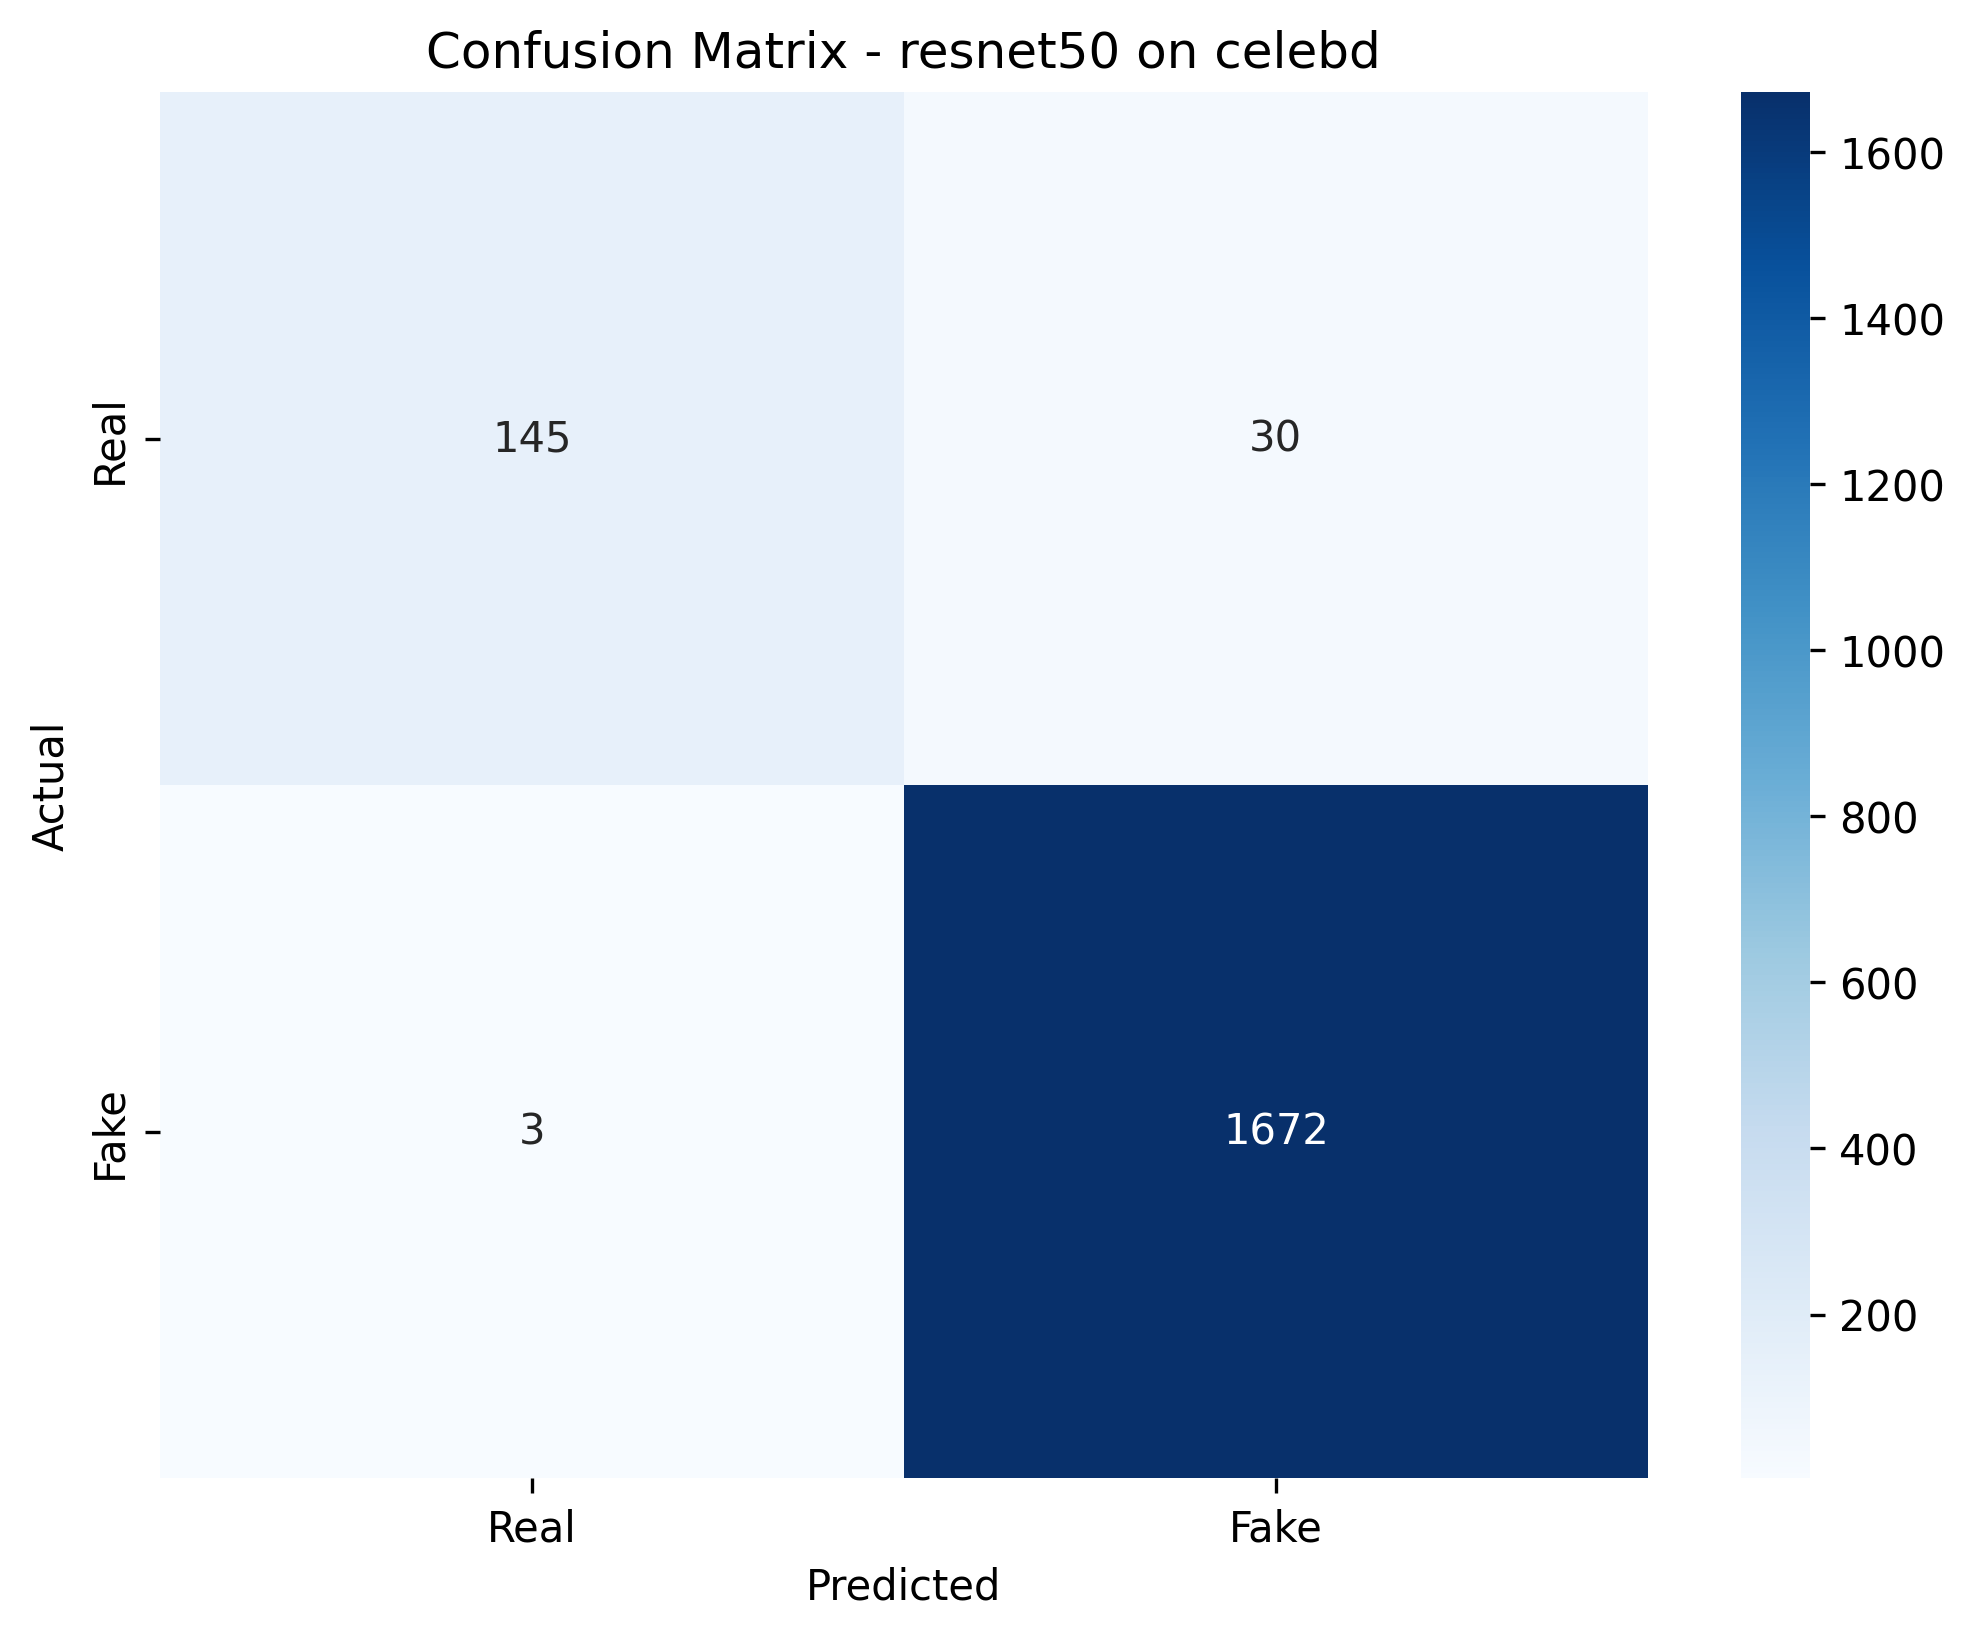
\includegraphics[width=0.24\textwidth]{figures/resnet50_celebd_confusion_matrix.png} &
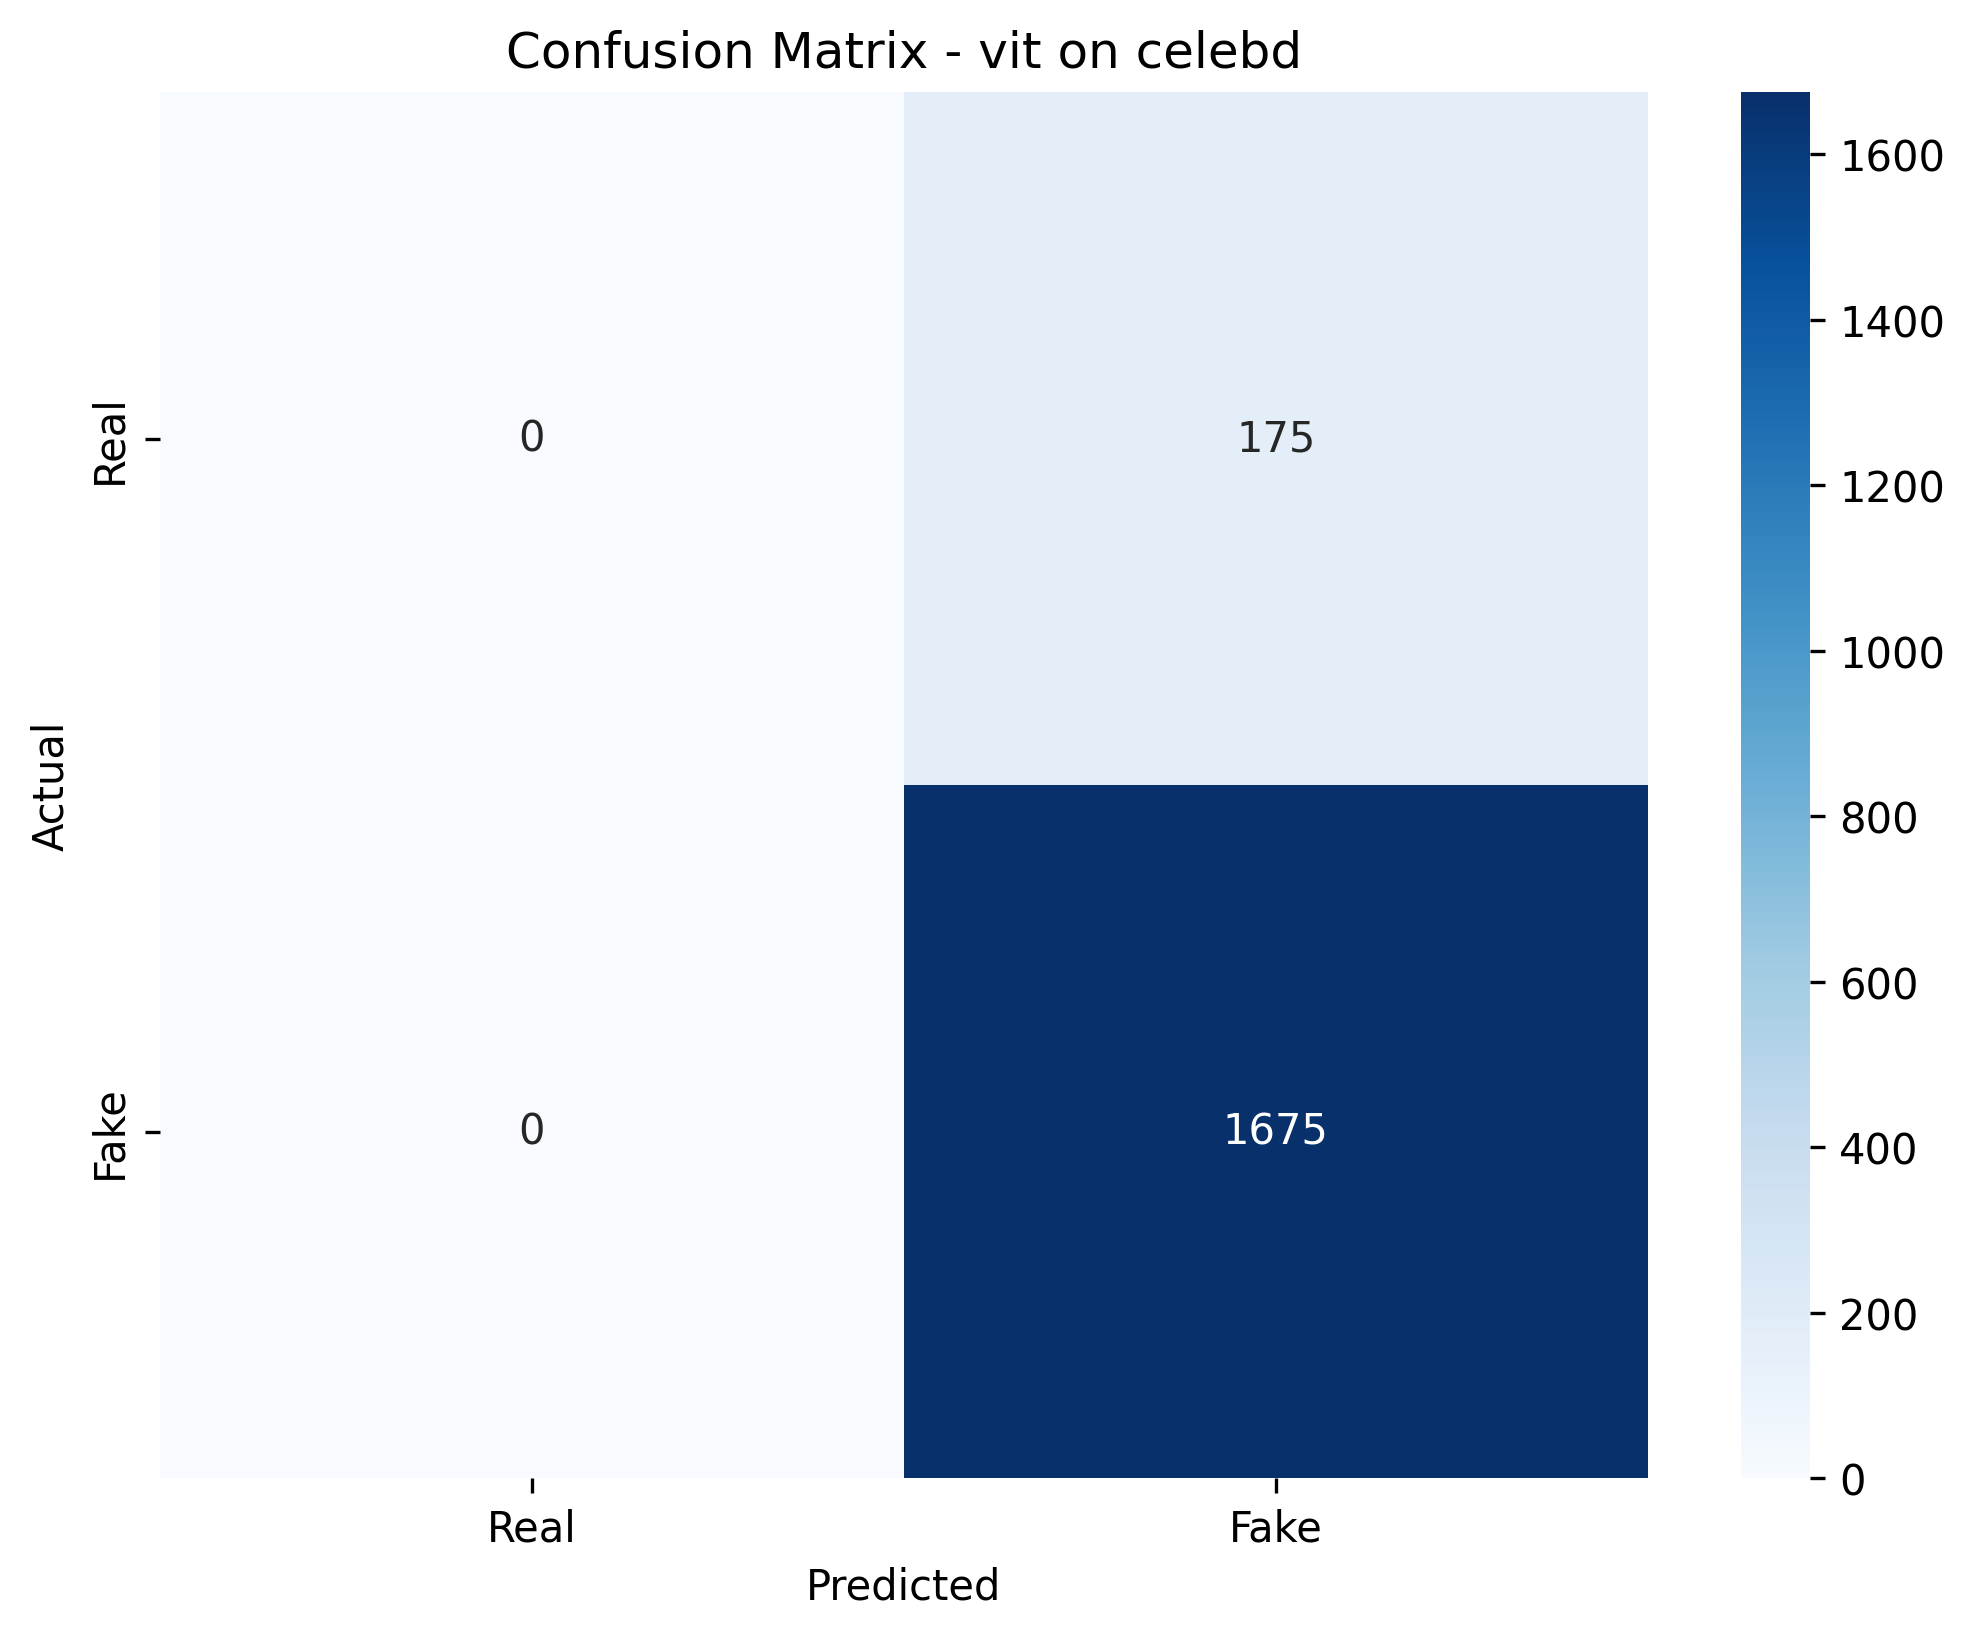
\includegraphics[width=0.24\textwidth]{figures/vit_celebd_confusion_matrix.png} \\
(c) ResNet50 & (d) Vision Transformer
\end{tabular}
\caption{Confusion matrices for all four models on Celeb-DF test set.}
\label{fig:confusion_celebd}
\end{figure*}

Figure~\ref{fig:roc_celebd} presents the ROC curves, demonstrating the trade-off between true positive rate and false positive rate across different classification thresholds. All CNN-based models achieve AUC values above 98\%, while the Vision Transformer shows lower AUC performance.

\begin{figure*}[!t]
\centering
\begin{tabular}{cc}
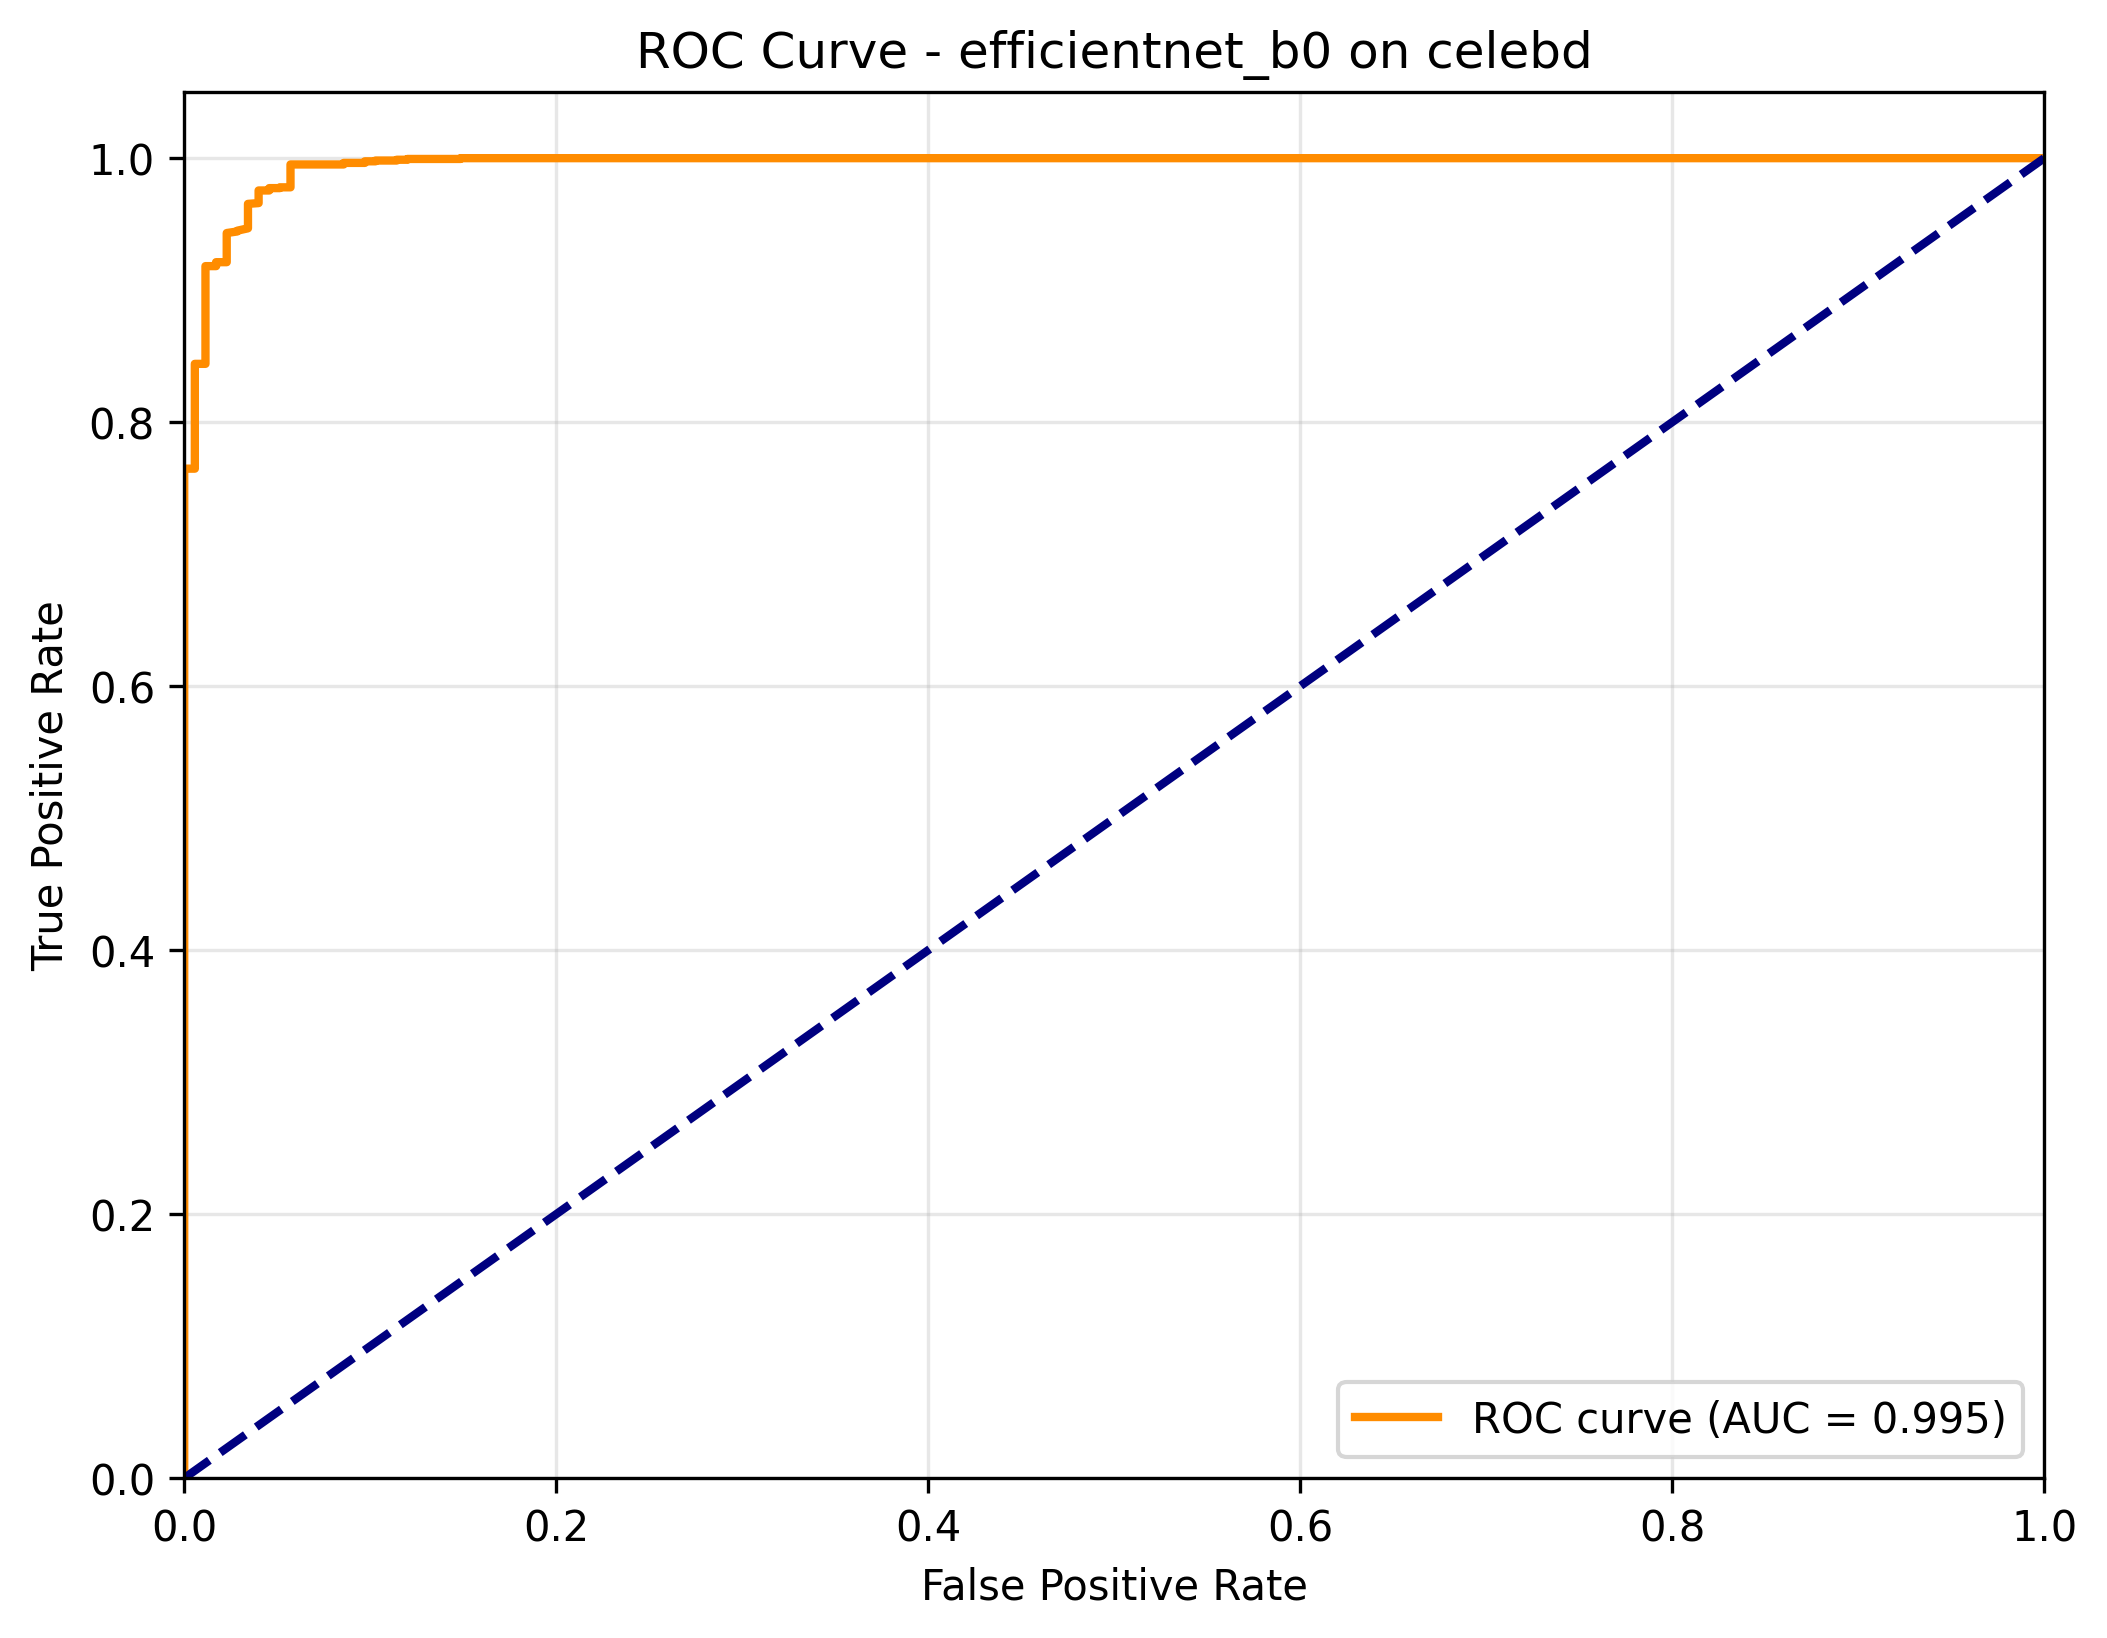
\includegraphics[width=0.24\textwidth]{figures/efficientnet_b0_celebd_roc_curve.png} &
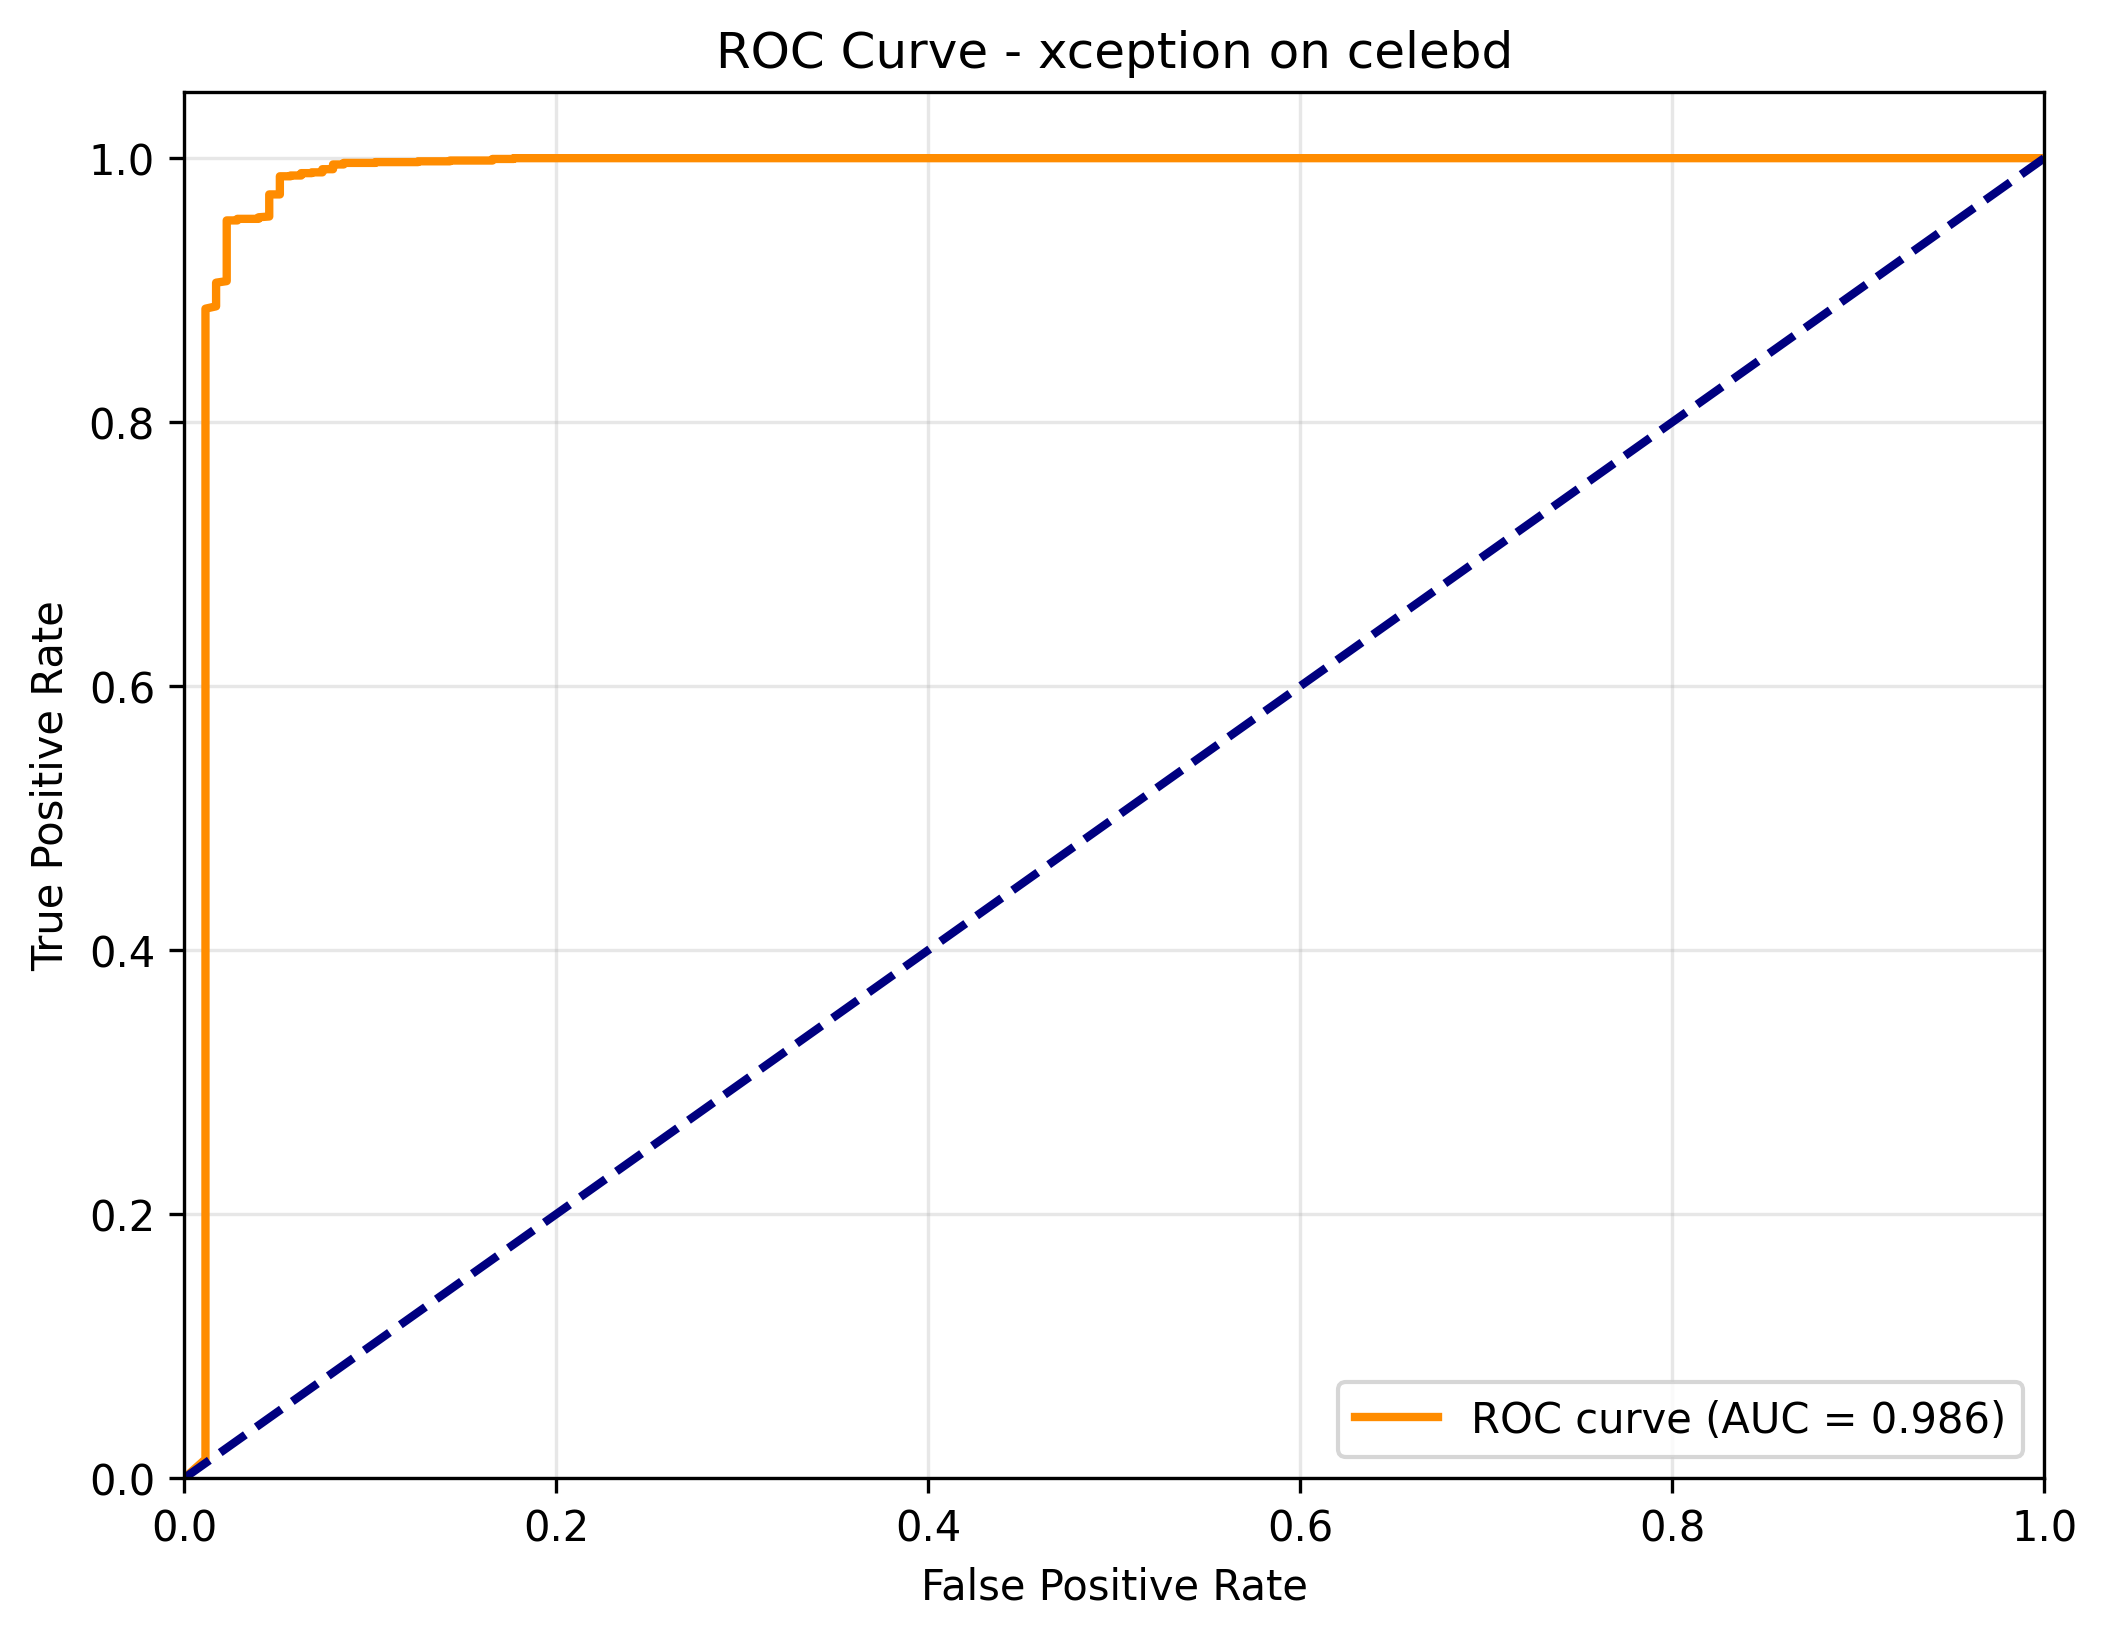
\includegraphics[width=0.24\textwidth]{figures/xception_celebd_roc_curve.png} \\
(a) EfficientNet-B0 & (b) XceptionNet \\
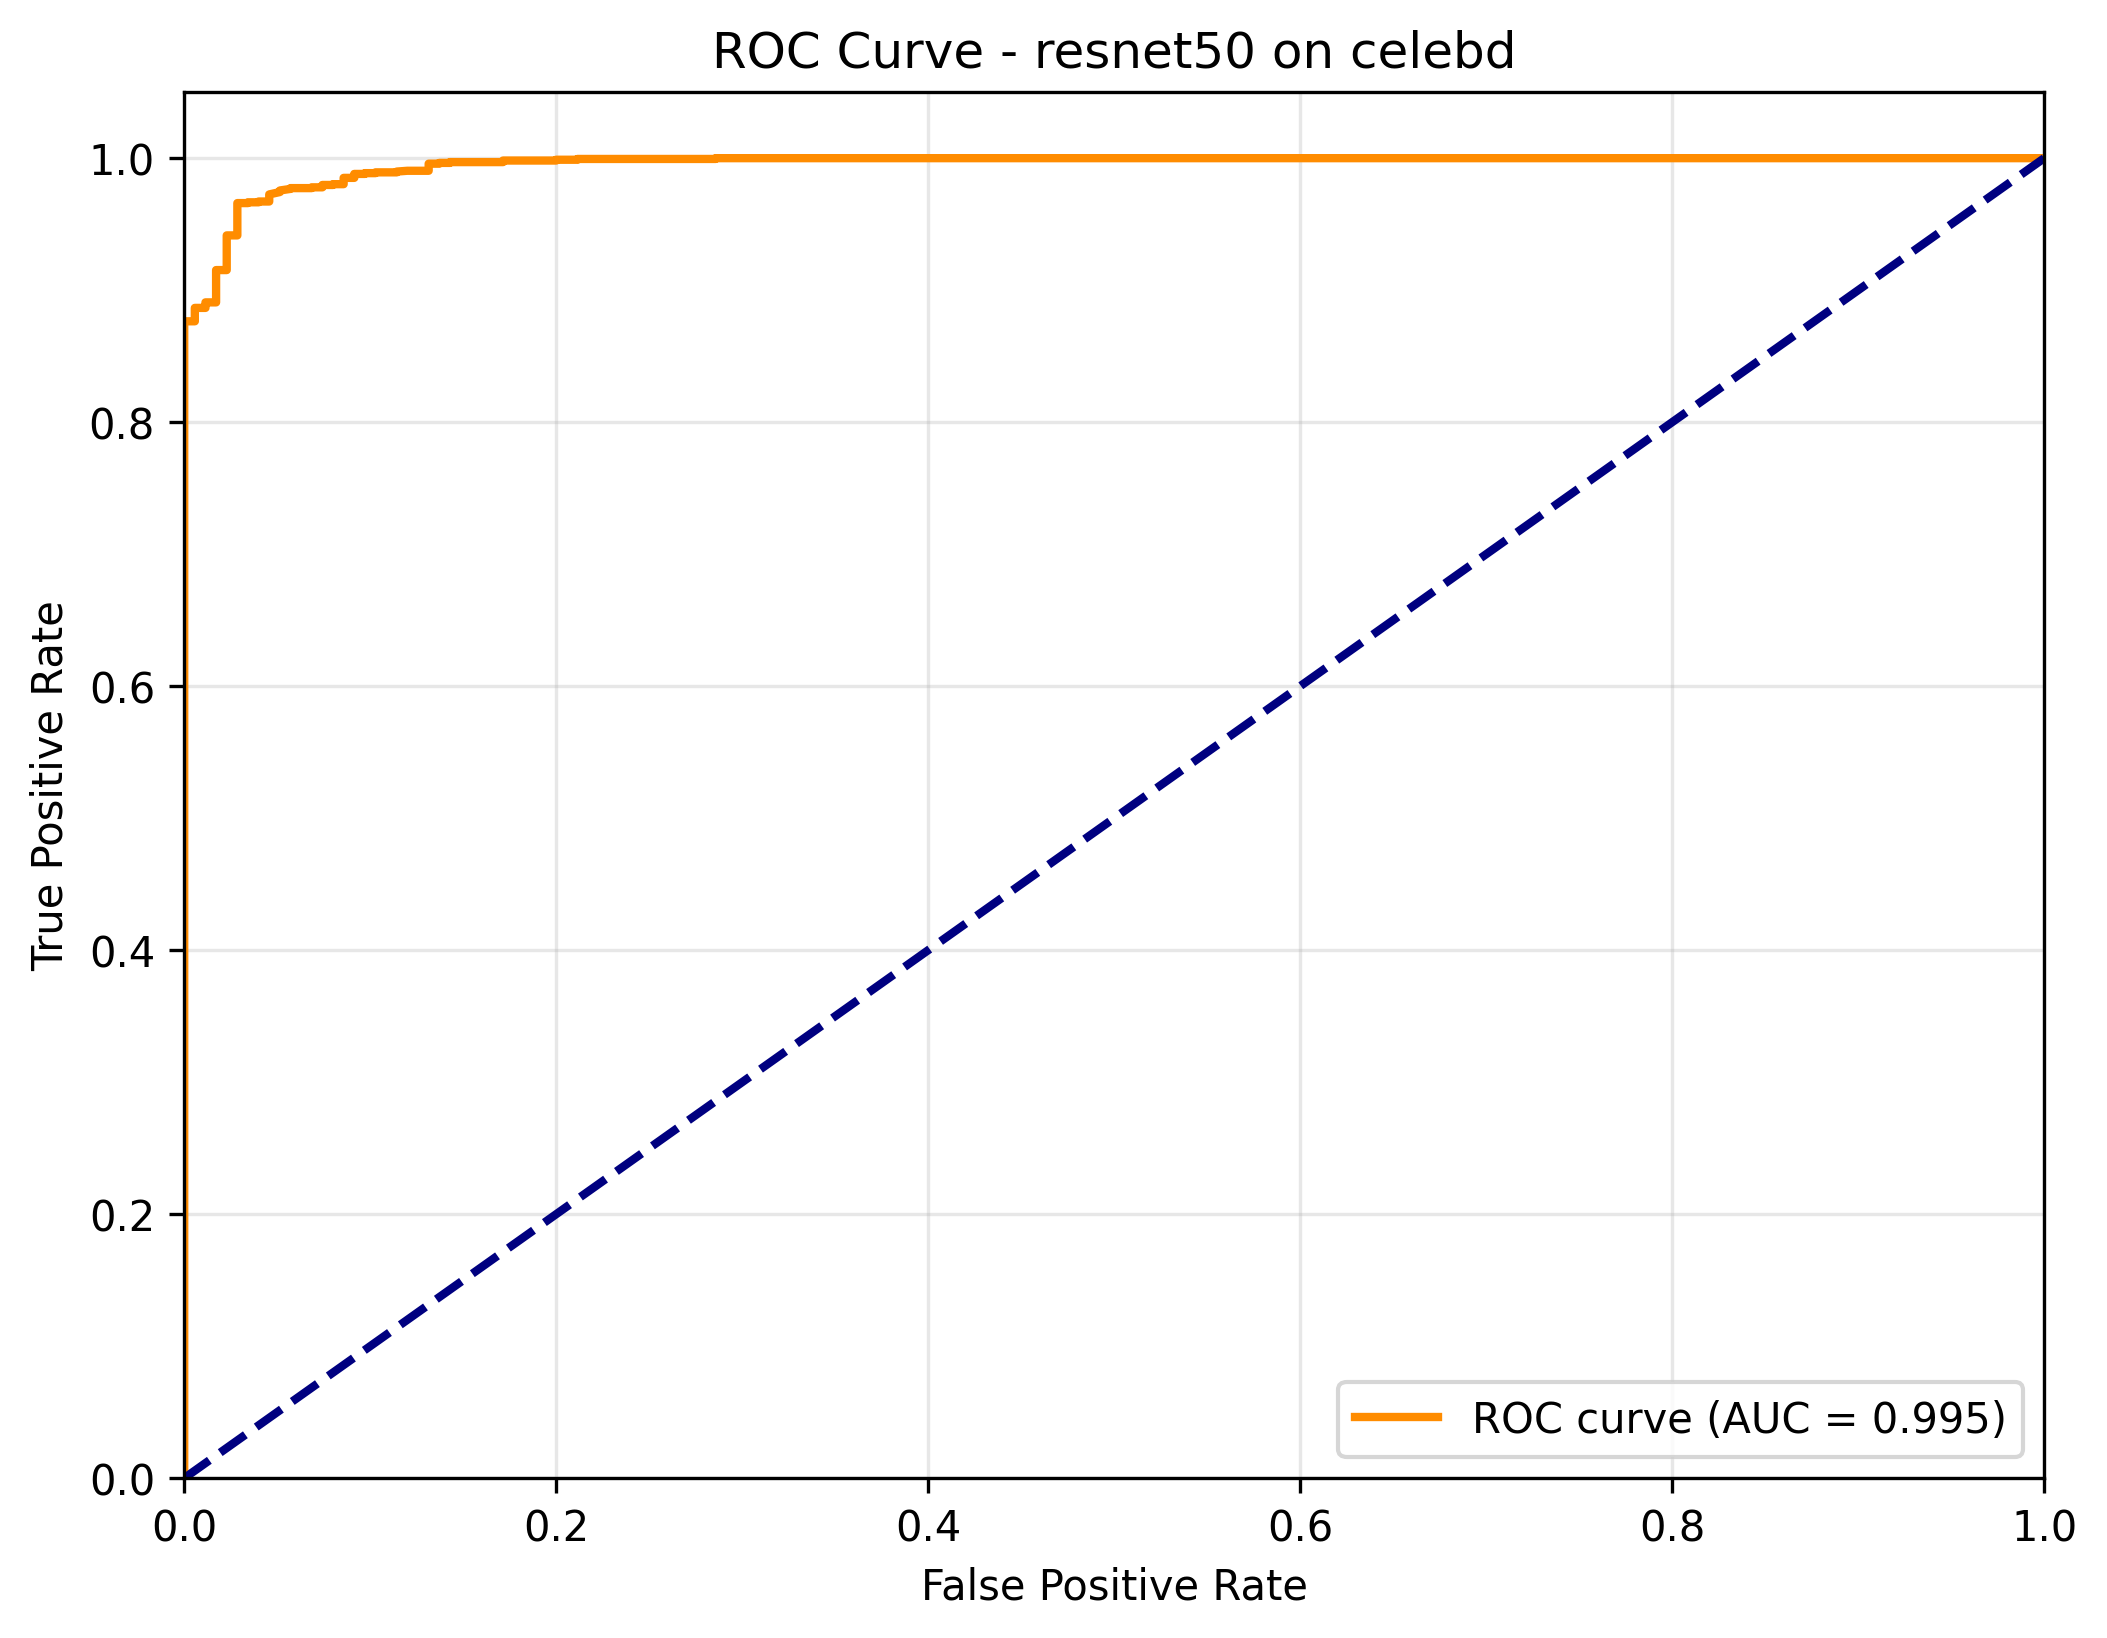
\includegraphics[width=0.24\textwidth]{figures/resnet50_celebd_roc_curve.png} &
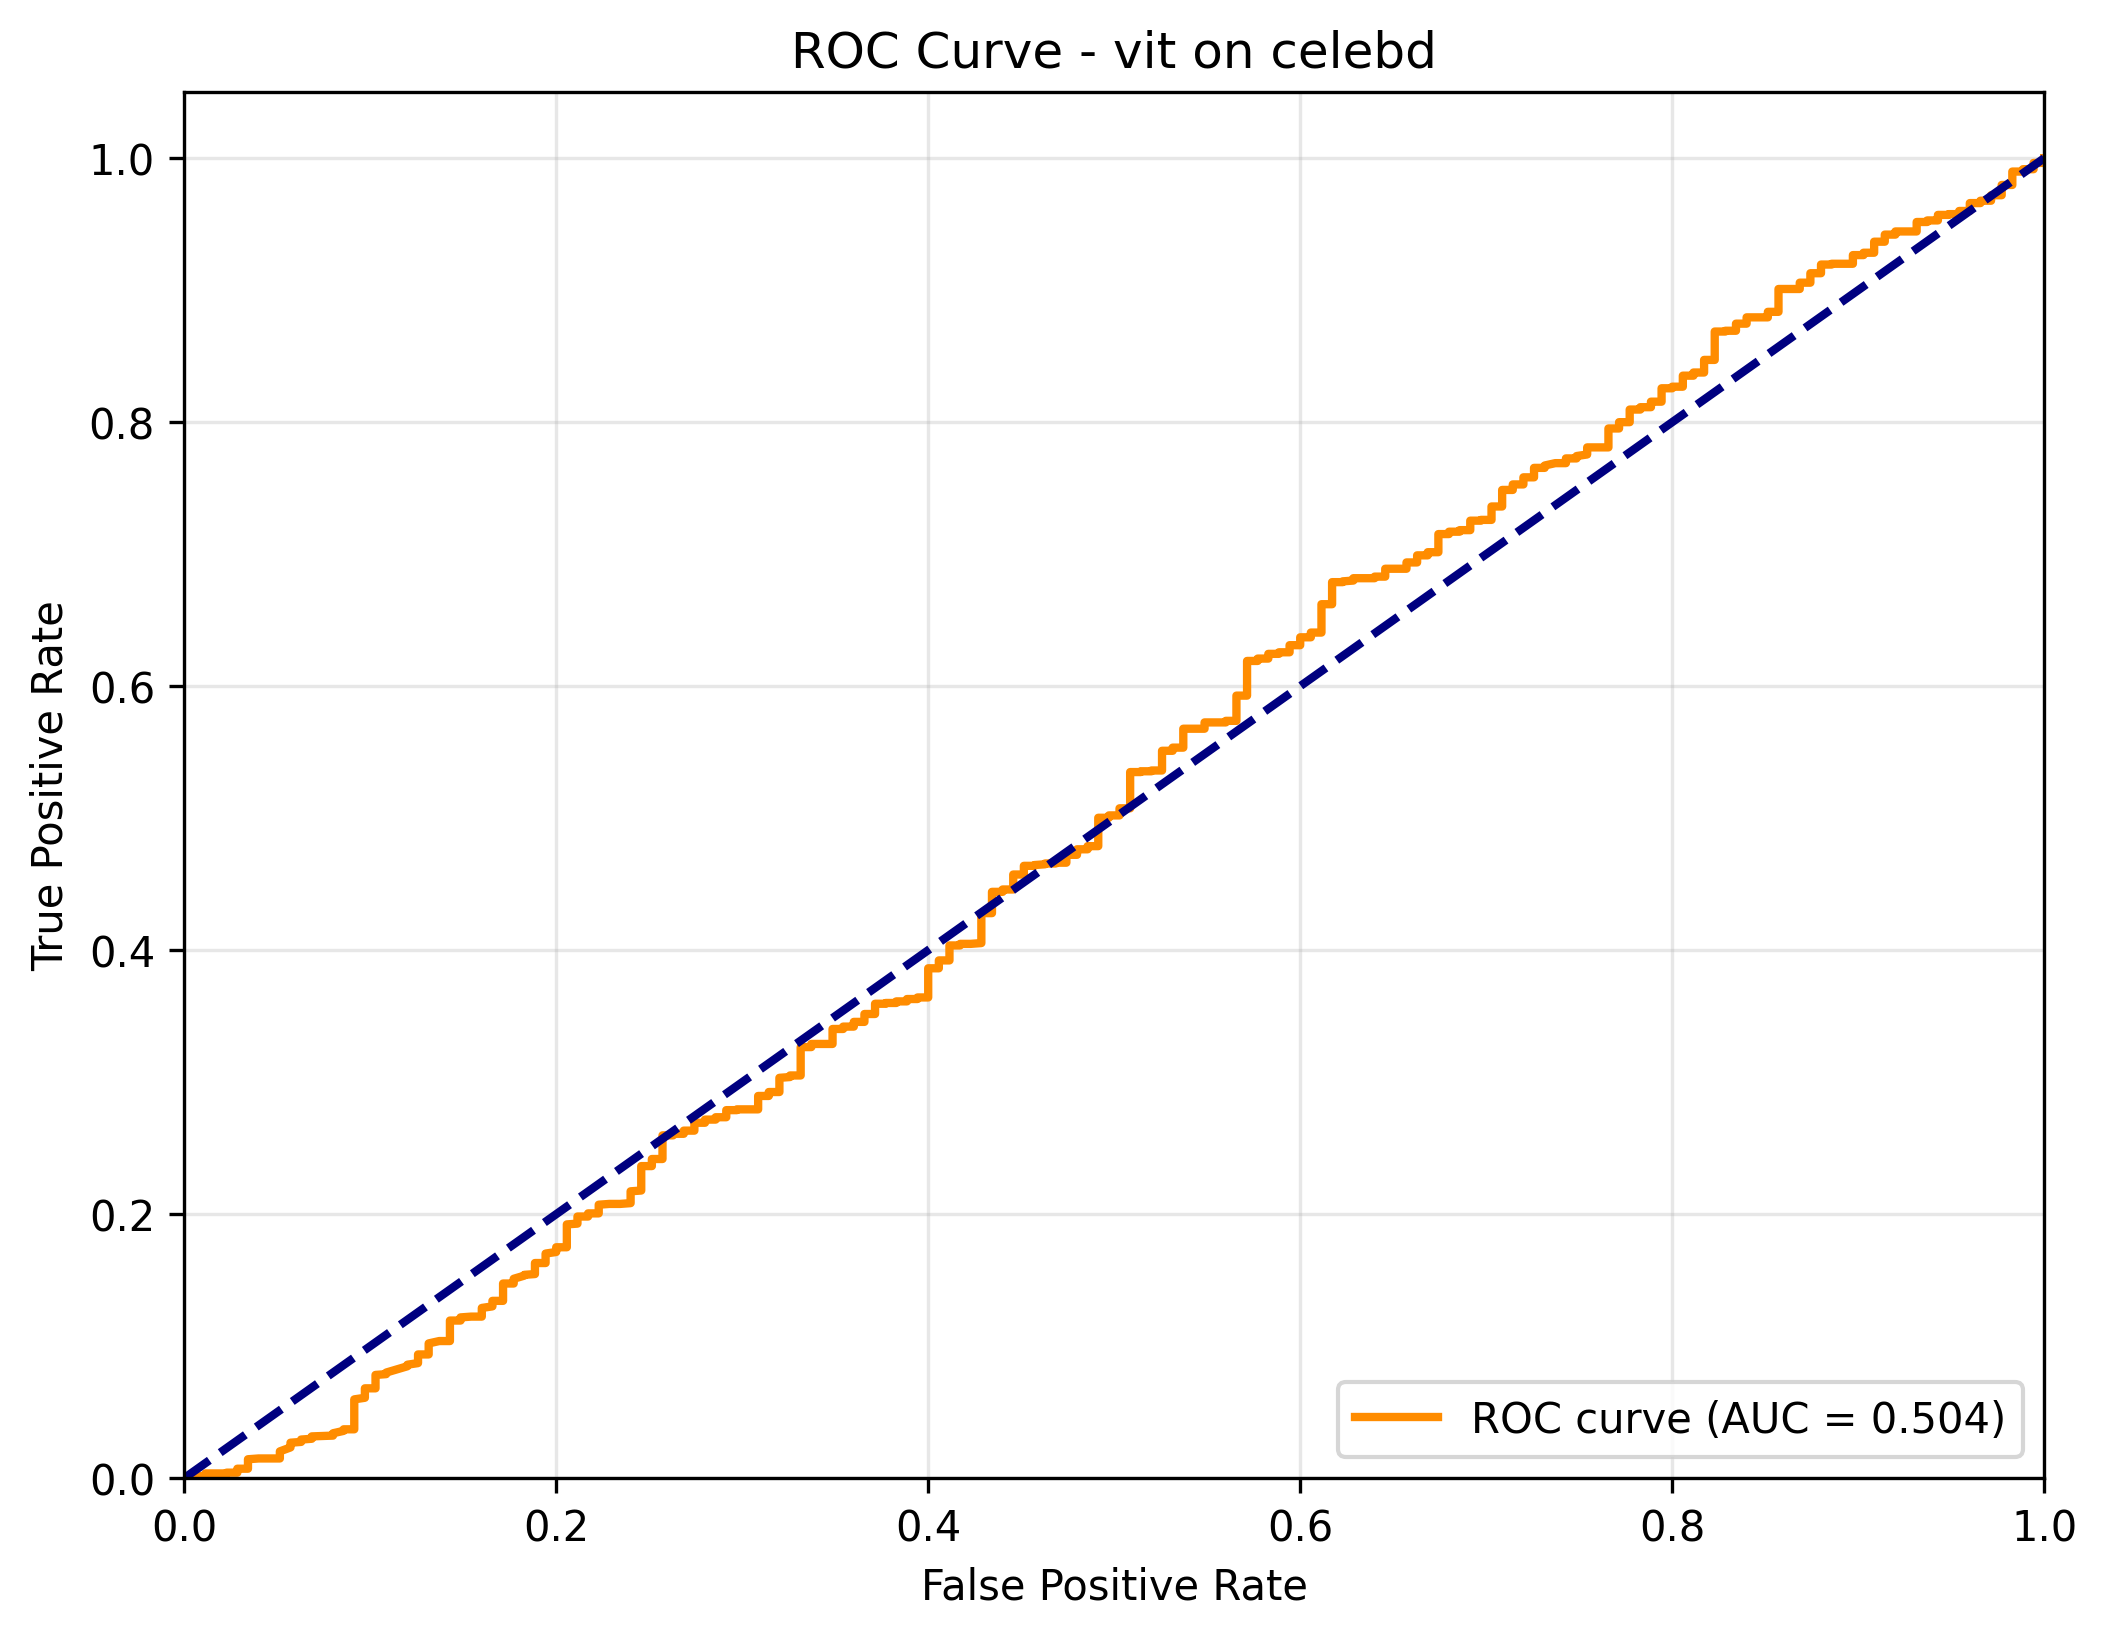
\includegraphics[width=0.24\textwidth]{figures/vit_celebd_roc_curve.png} \\
(c) ResNet50 & (d) Vision Transformer
\end{tabular}
\caption{ROC curves for all four models on Celeb-DF test set.}
\label{fig:roc_celebd}
\end{figure*}

Figure~\ref{fig:pr_celebd} shows the precision-recall curves, which provide complementary insights to ROC curves, particularly useful for imbalanced datasets. These curves illustrate the relationship between precision and recall at different classification thresholds.

\begin{figure*}[!t]
\centering
\begin{tabular}{cc}
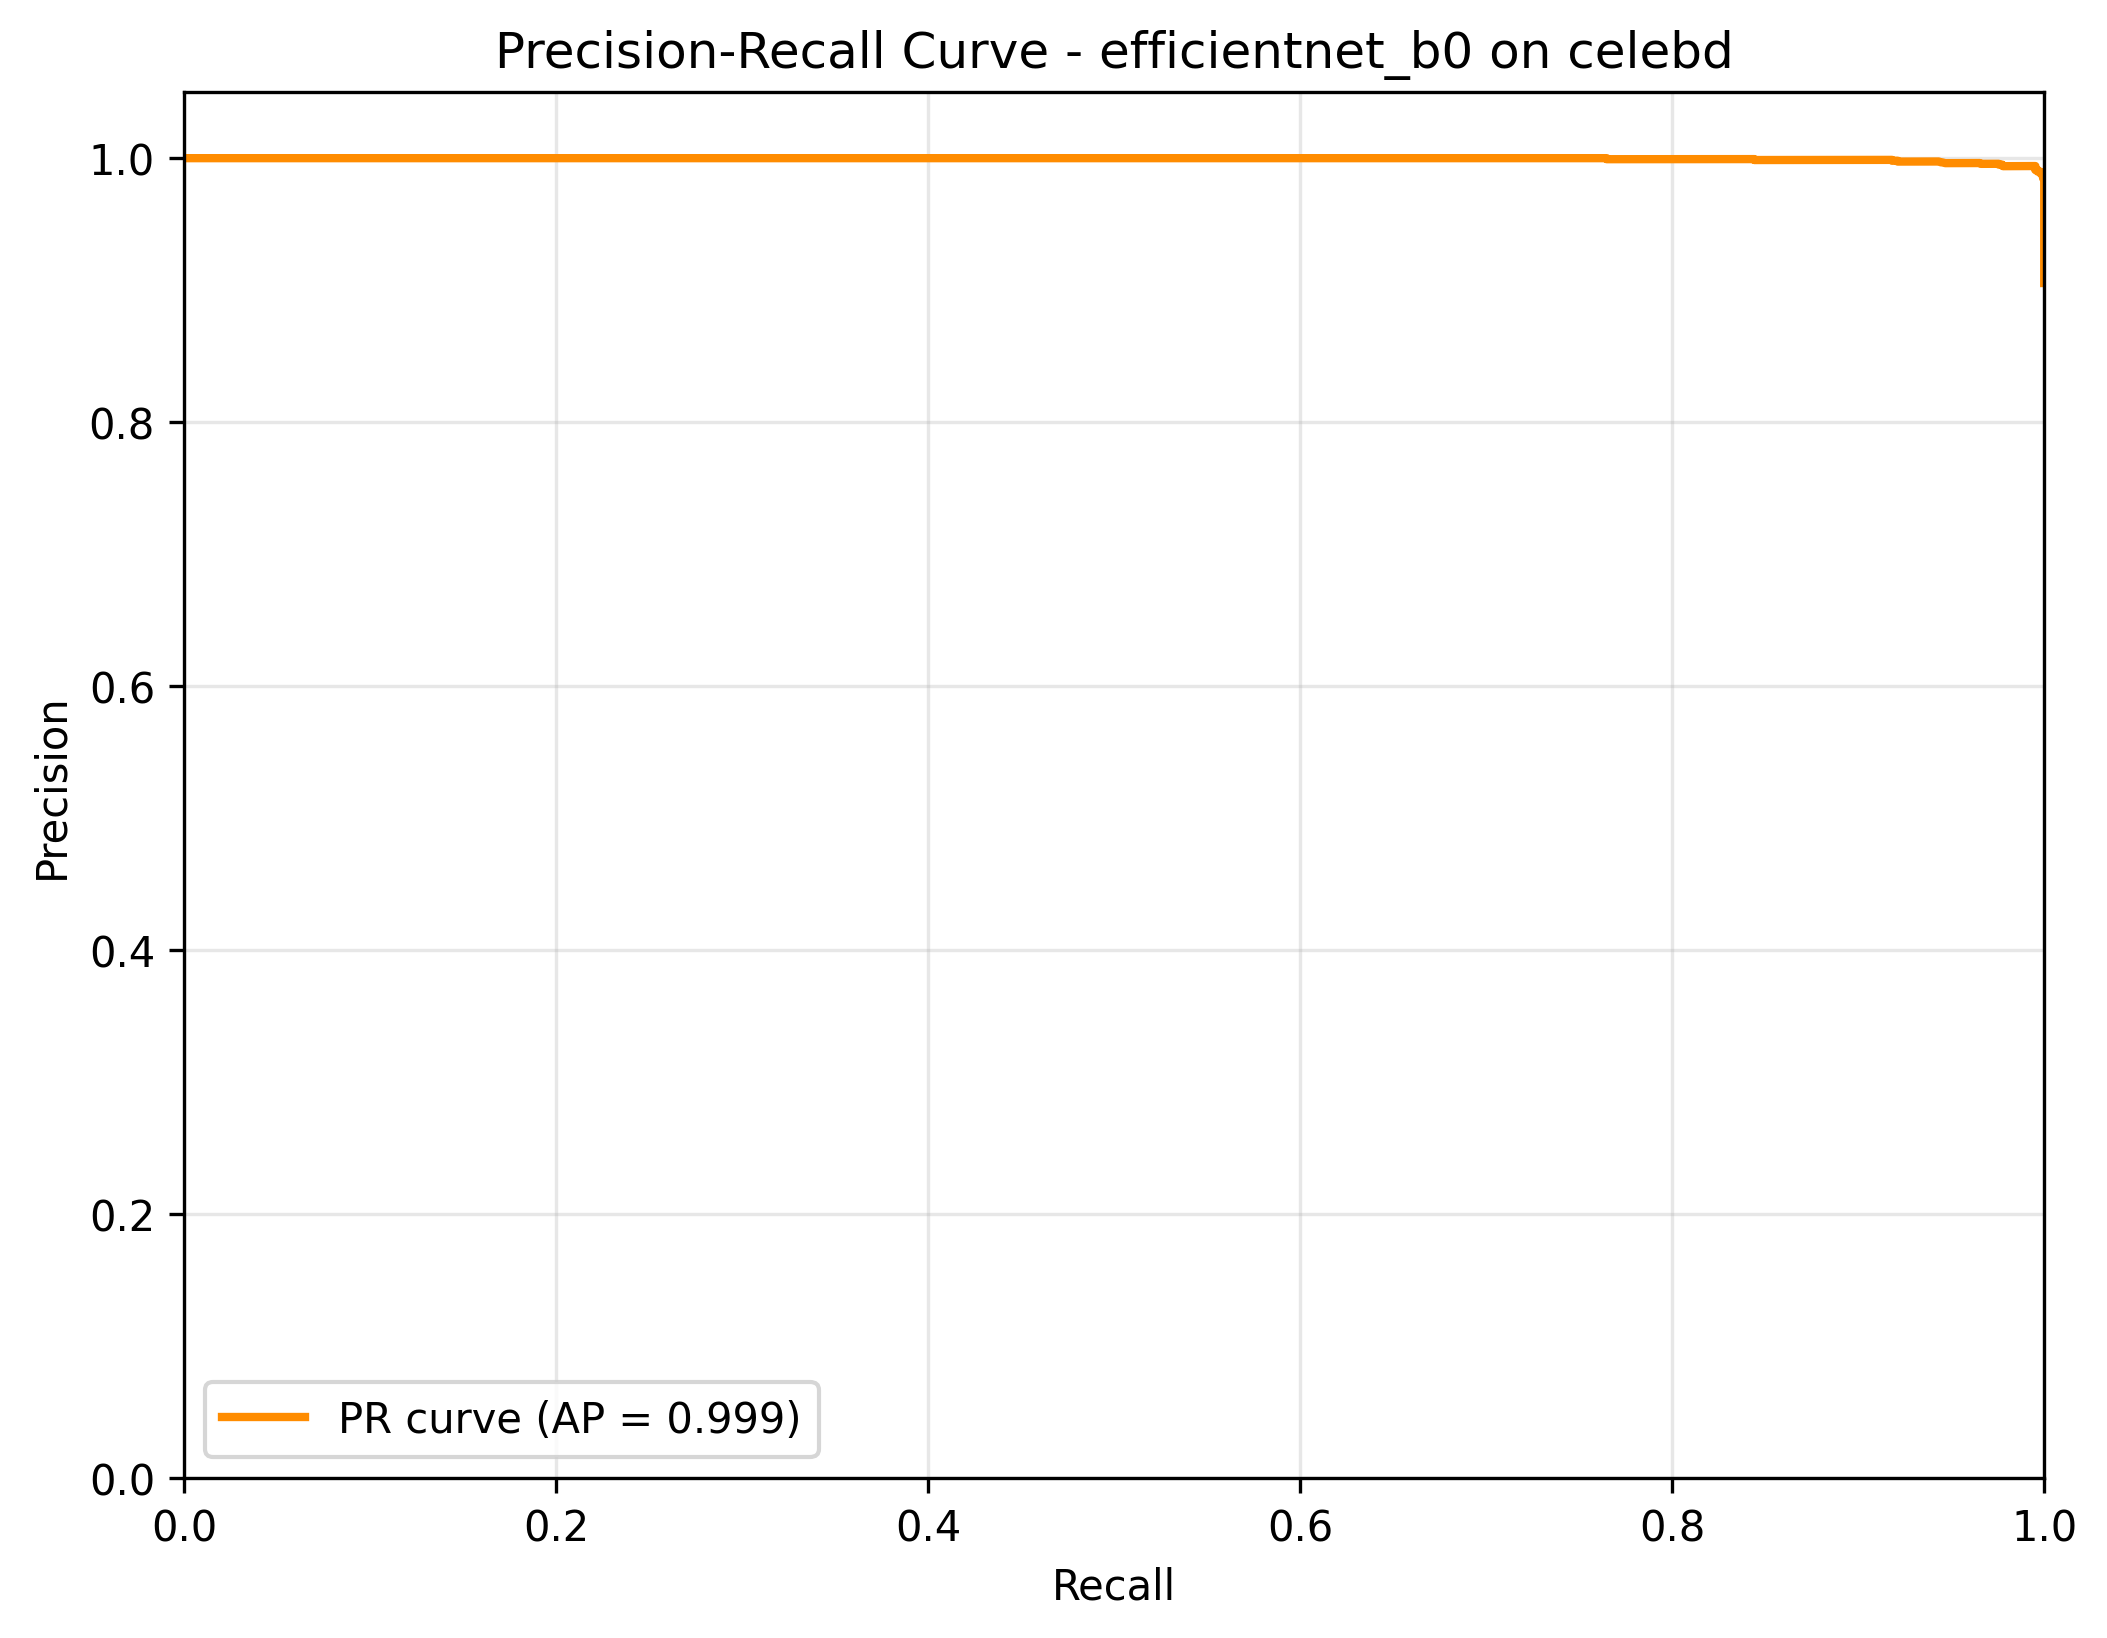
\includegraphics[width=0.24\textwidth]{figures/efficientnet_b0_celebd_precision_recall_curve.png} &
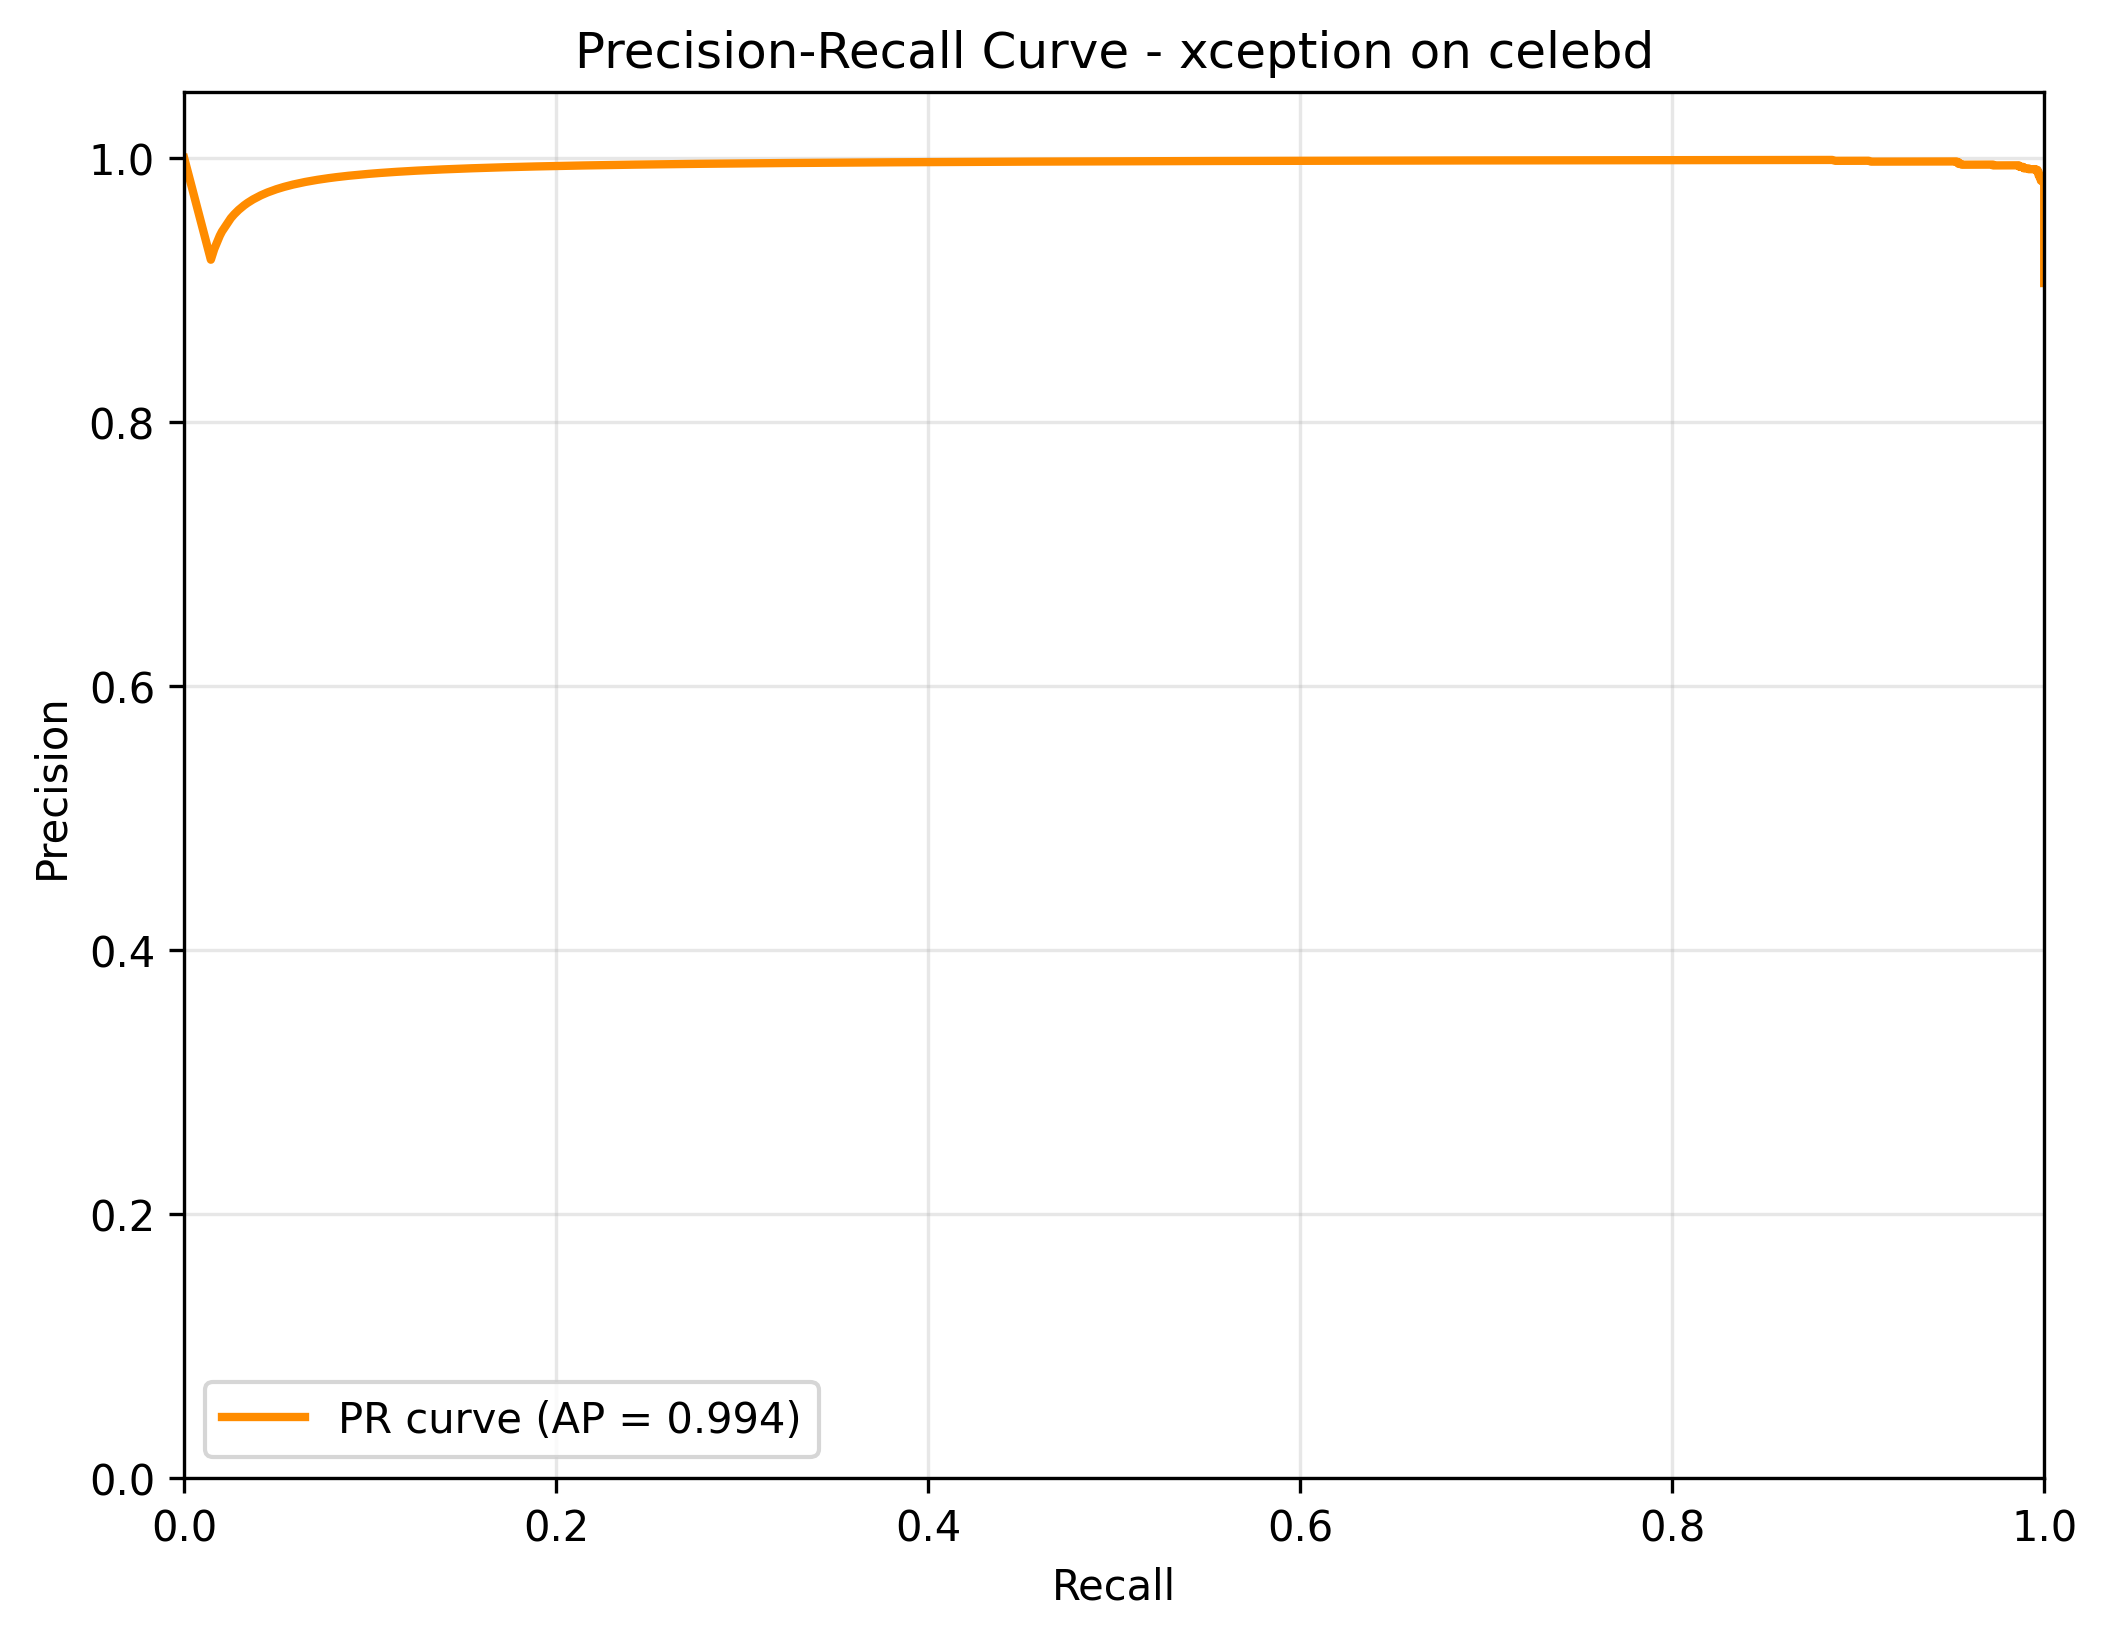
\includegraphics[width=0.24\textwidth]{figures/xception_celebd_precision_recall_curve.png} \\
(a) EfficientNet-B0 & (b) XceptionNet \\
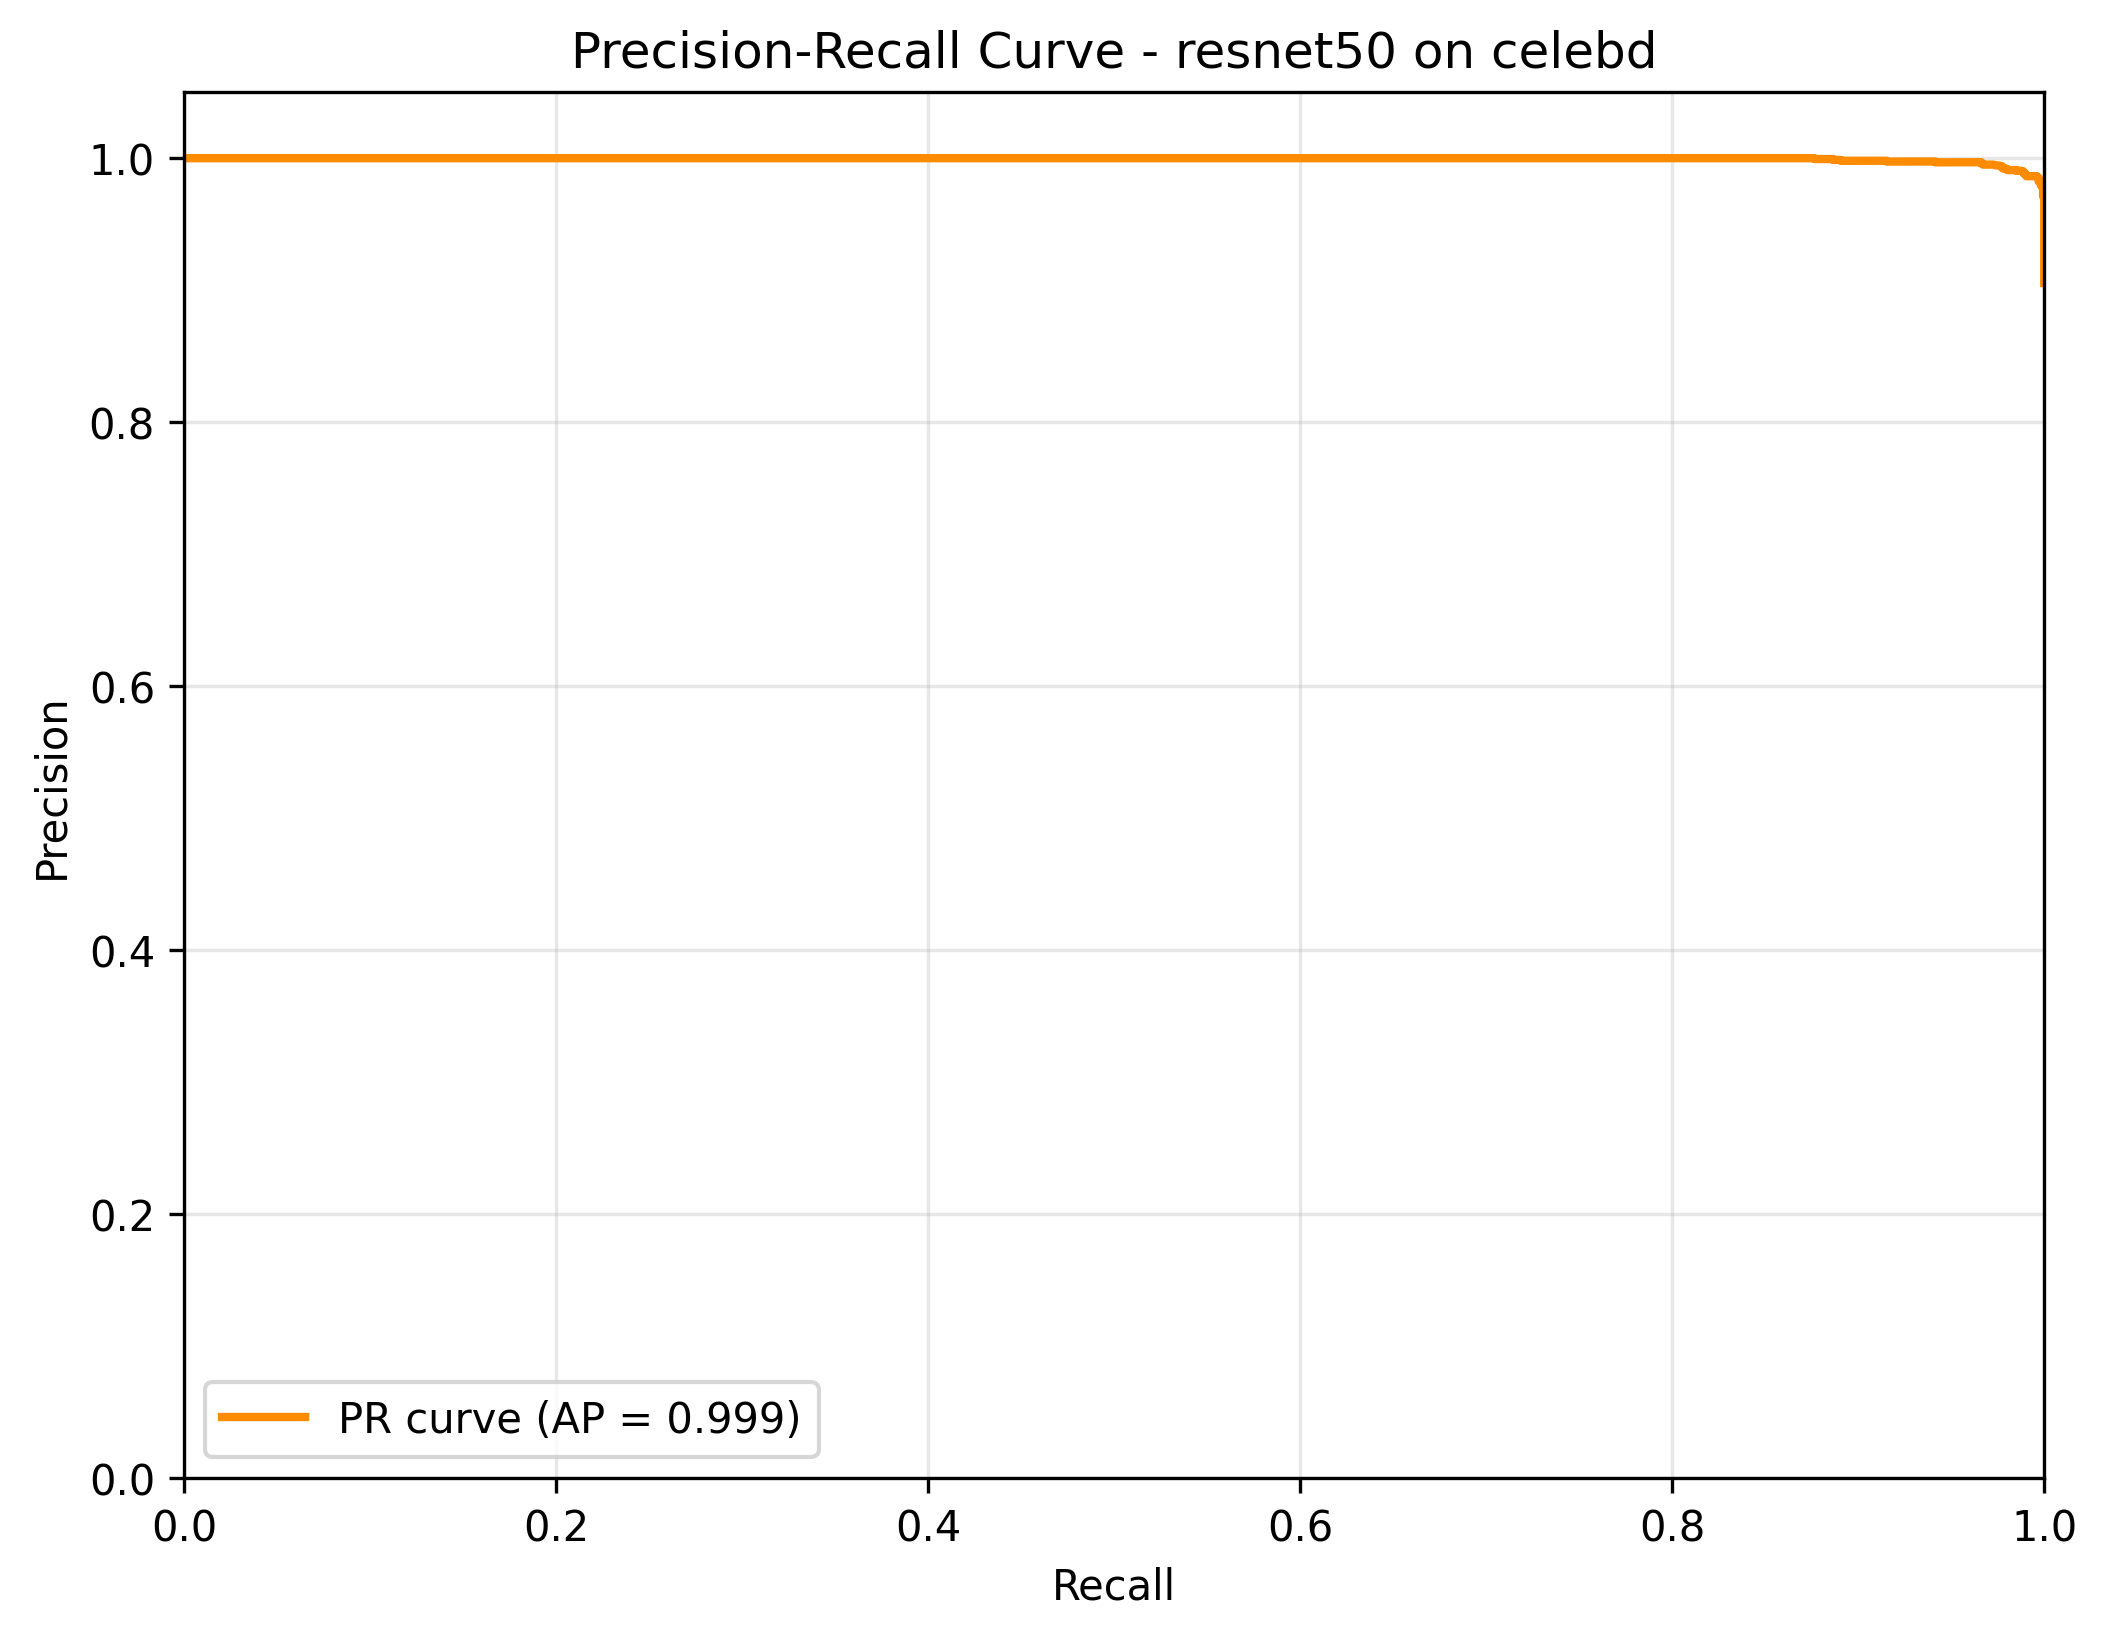
\includegraphics[width=0.24\textwidth]{figures/resnet50_celebd_precision_recall_curve.png} &
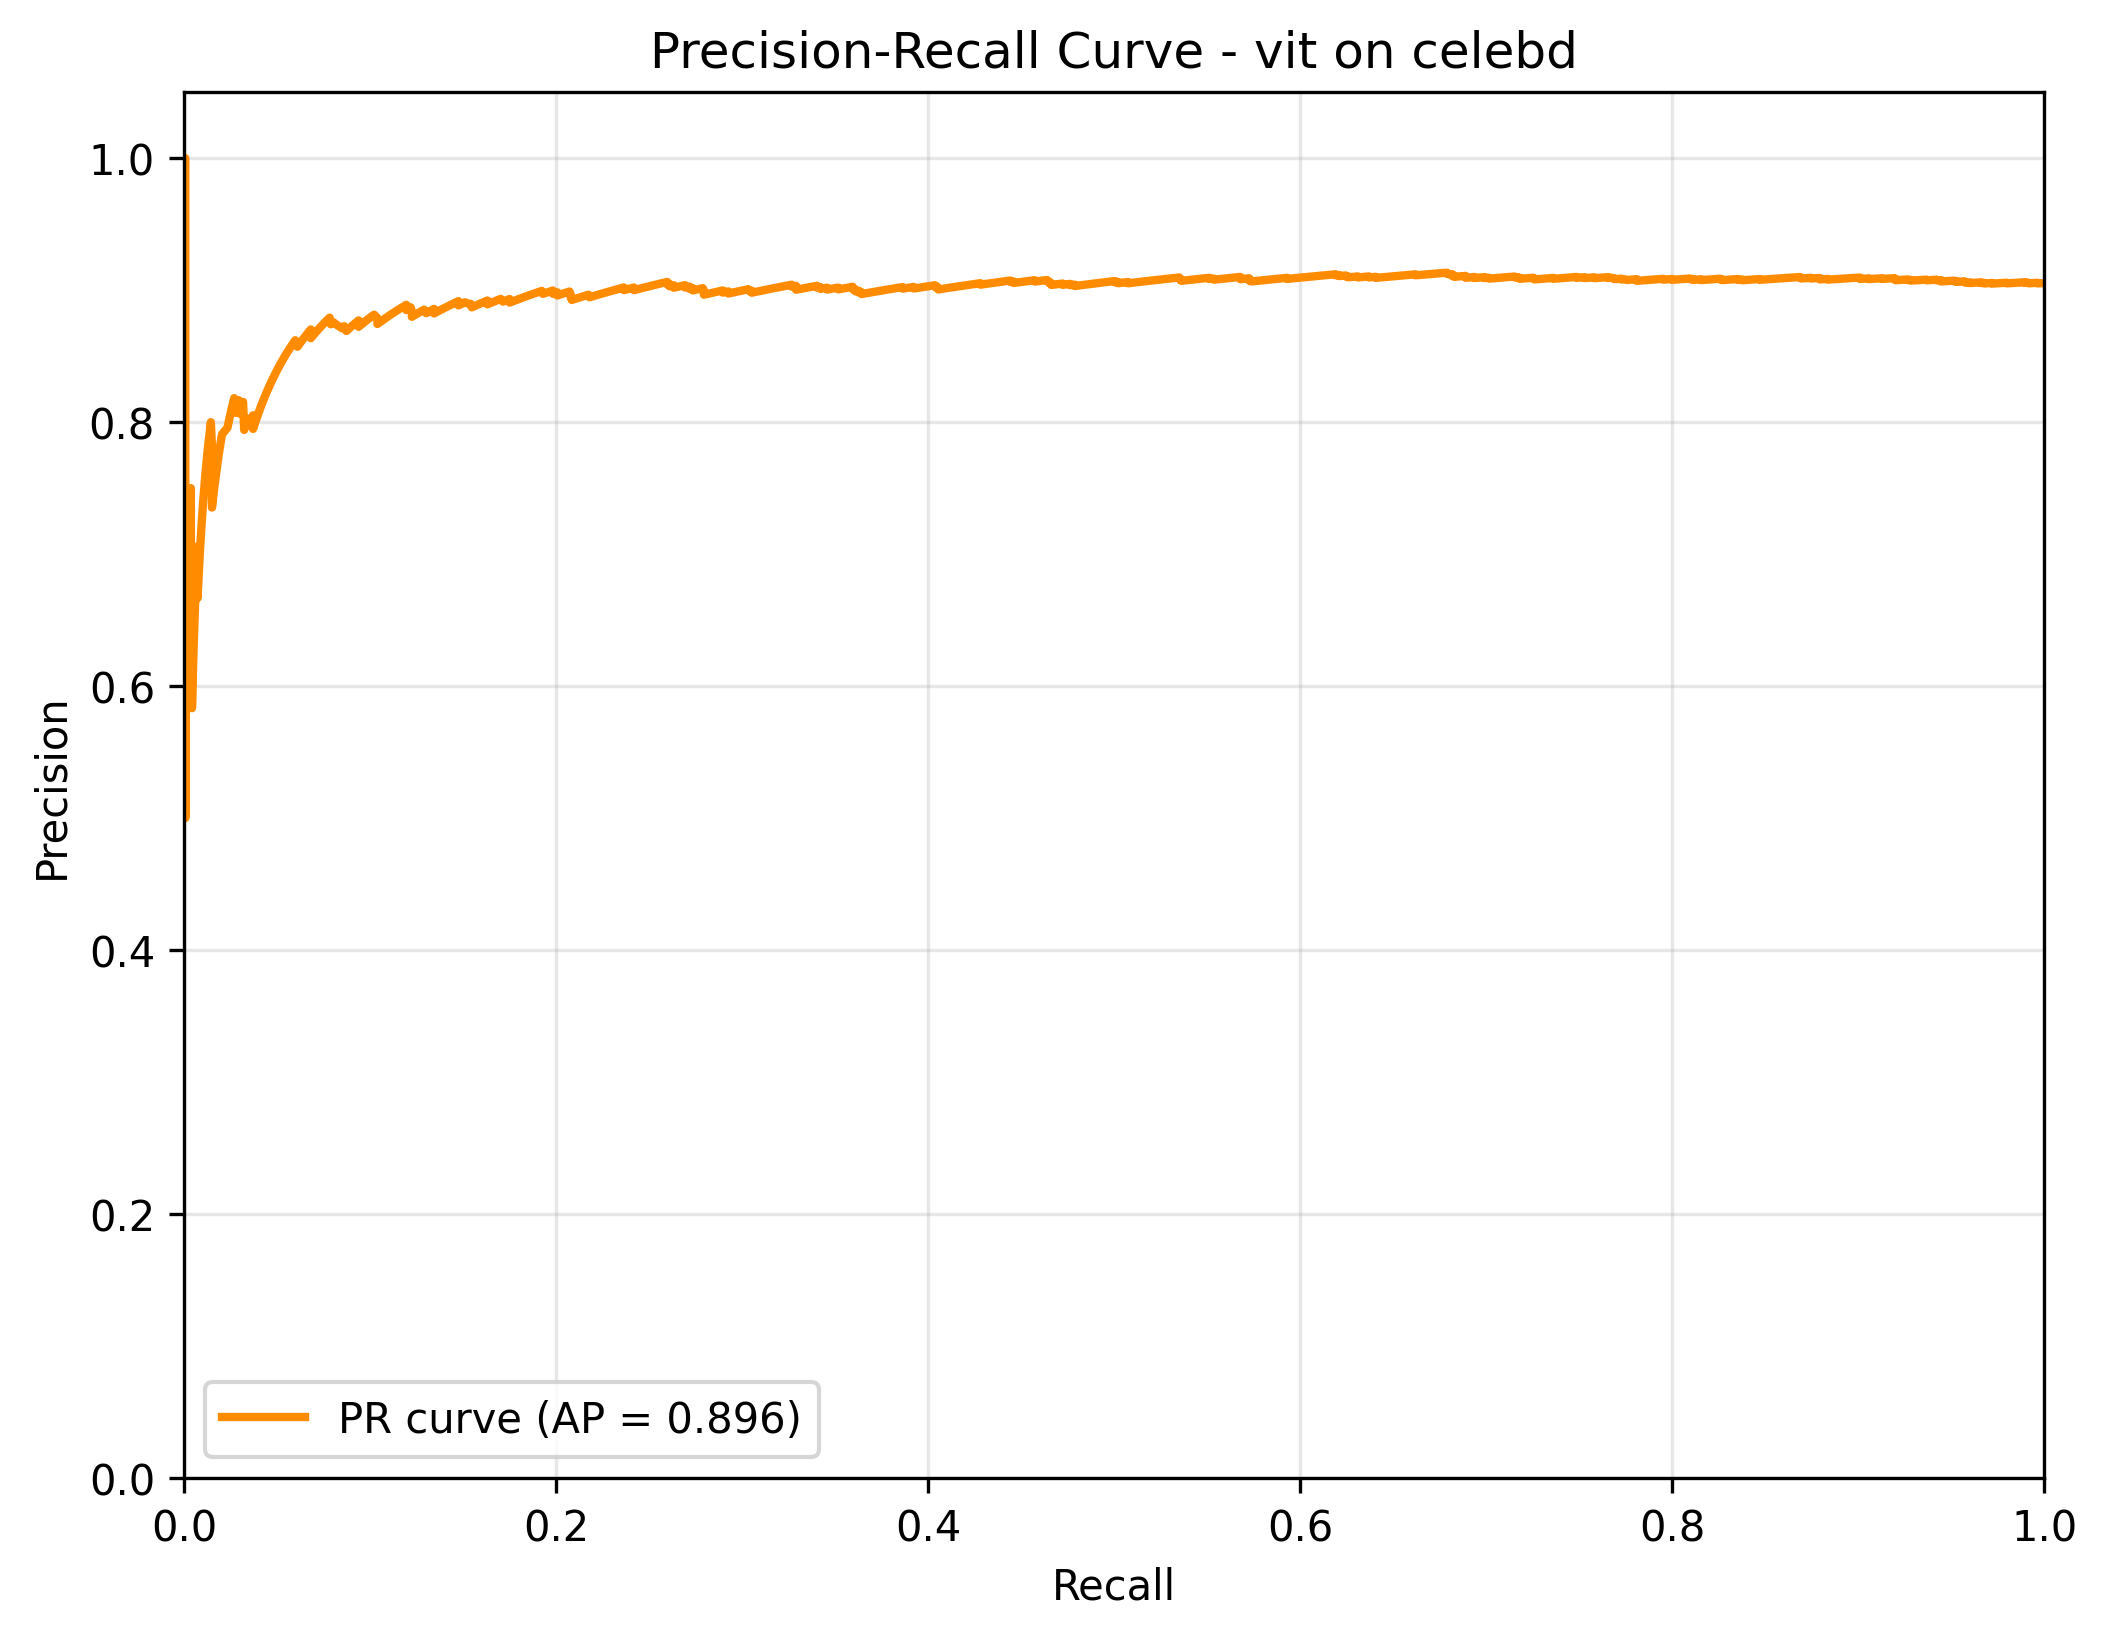
\includegraphics[width=0.24\textwidth]{figures/vit_celebd_precision_recall_curve.png} \\
(c) ResNet50 & (d) Vision Transformer
\end{tabular}
\caption{Precision-Recall curves for all four models on Celeb-DF test set.}
\label{fig:pr_celebd}
\end{figure*}

\subsection{Cross-Dataset Visualization}
Figure~\ref{fig:confusion_ff} shows confusion matrices for cross-dataset evaluation, clearly illustrating the performance degradation when models trained on Celeb-DF are tested on FaceForensics++.

\begin{figure*}[!t]
\centering
\begin{tabular}{cc}
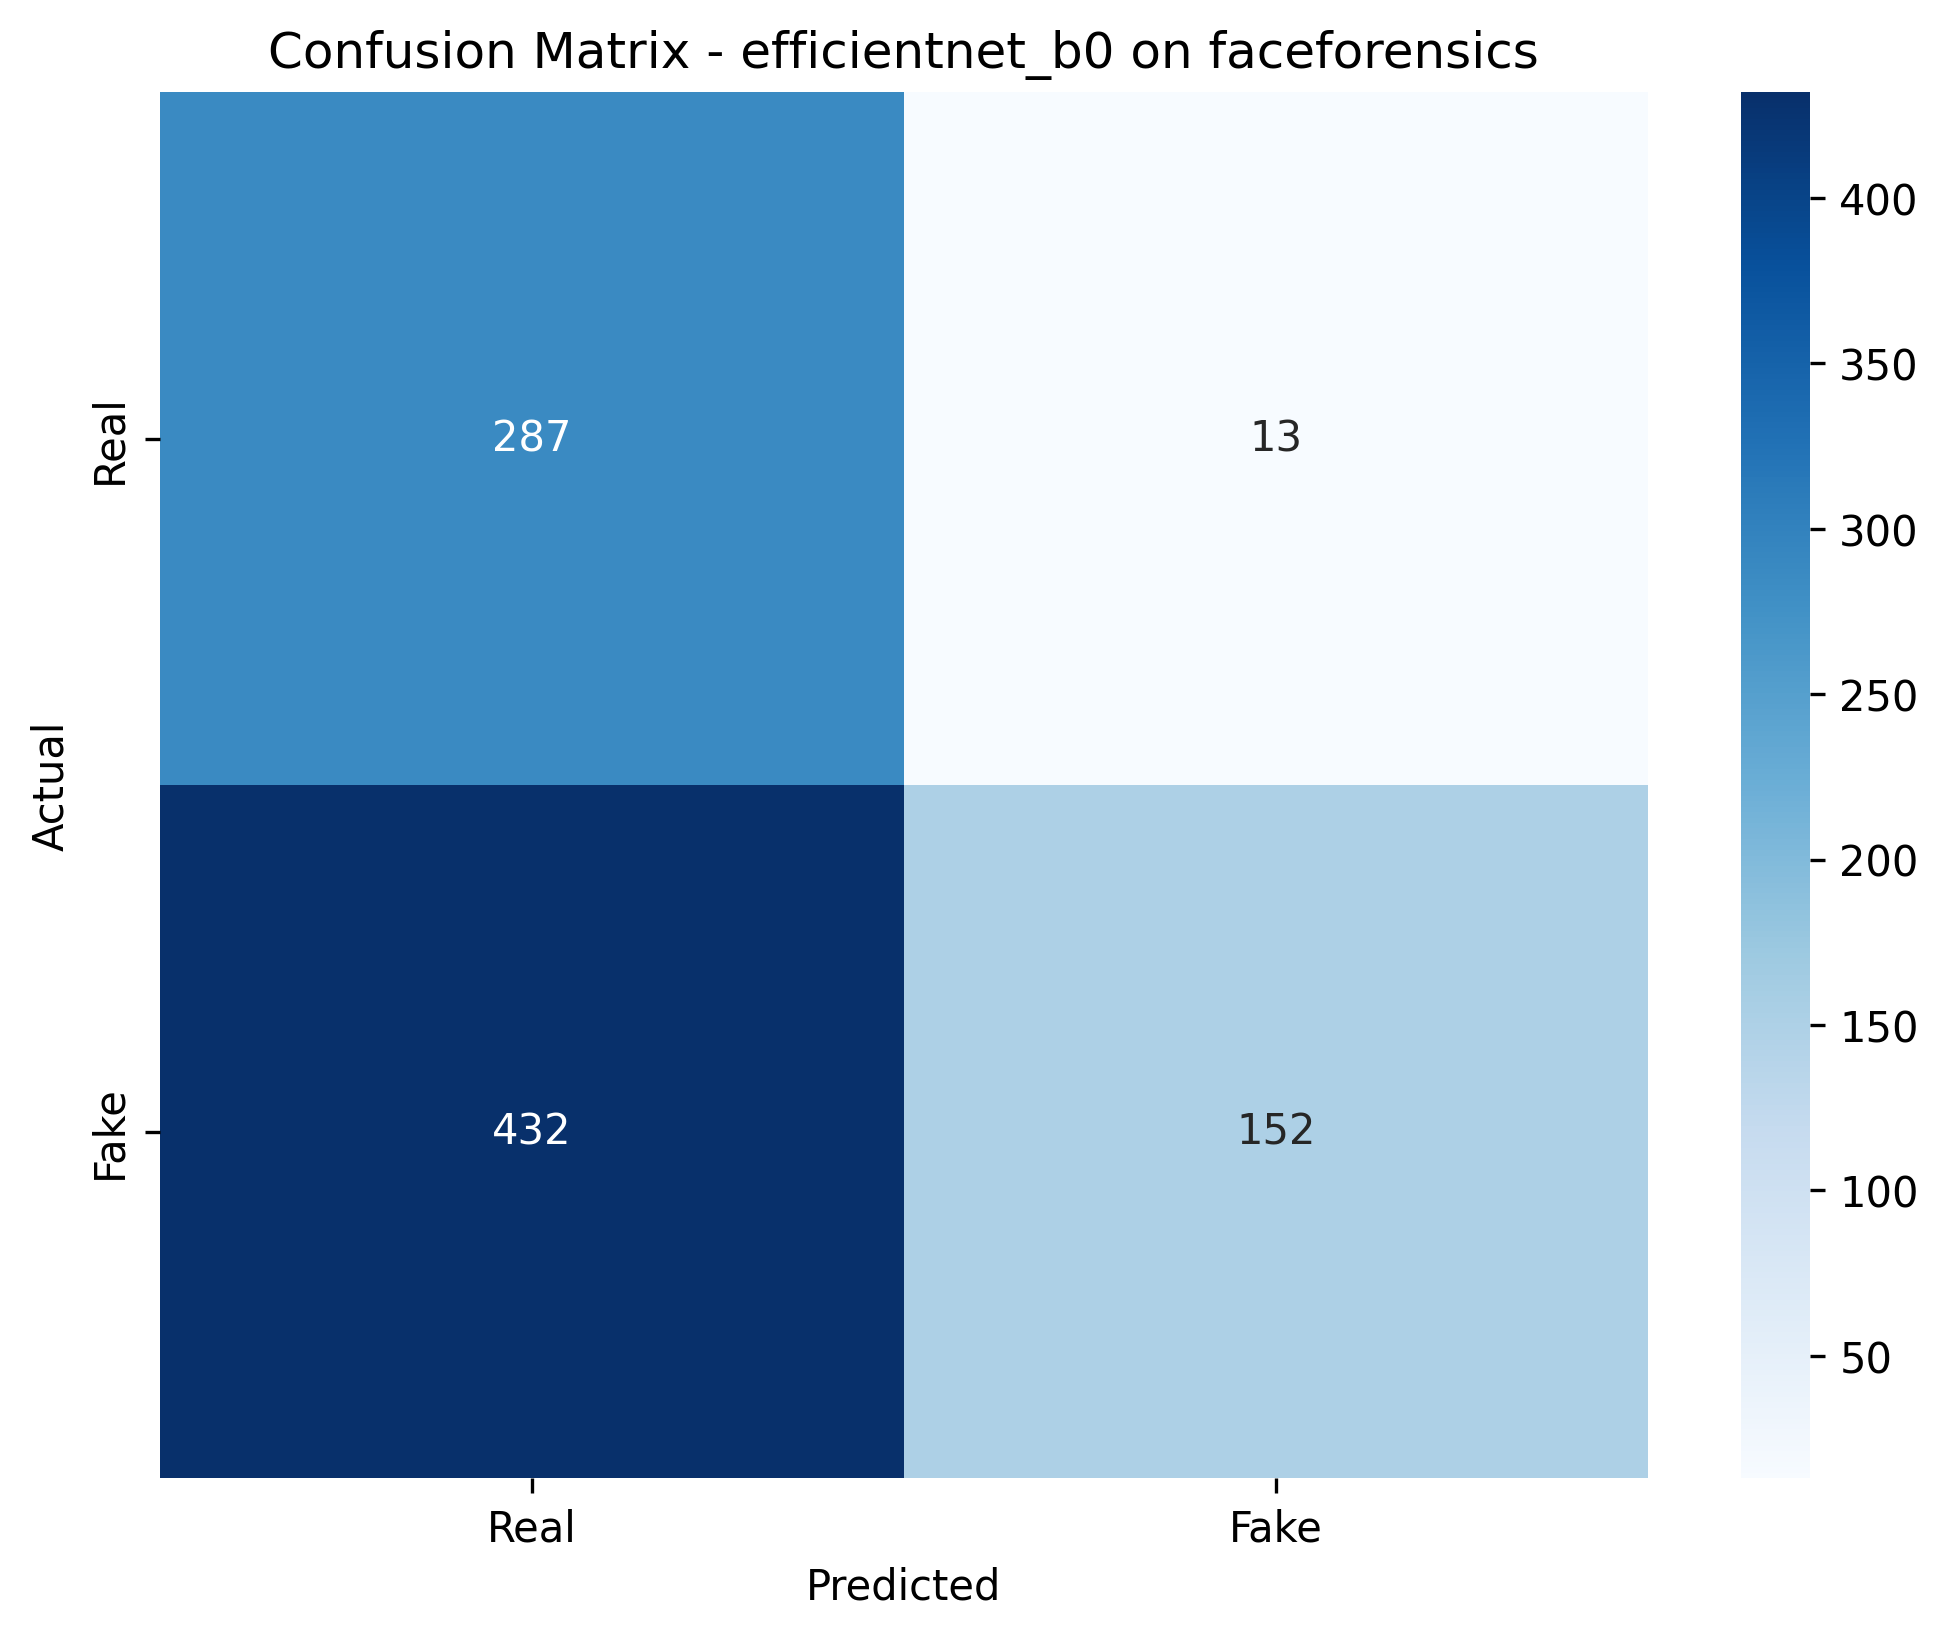
\includegraphics[width=0.24\textwidth]{figures/efficientnet_b0_faceforensics_confusion_matrix.png} &
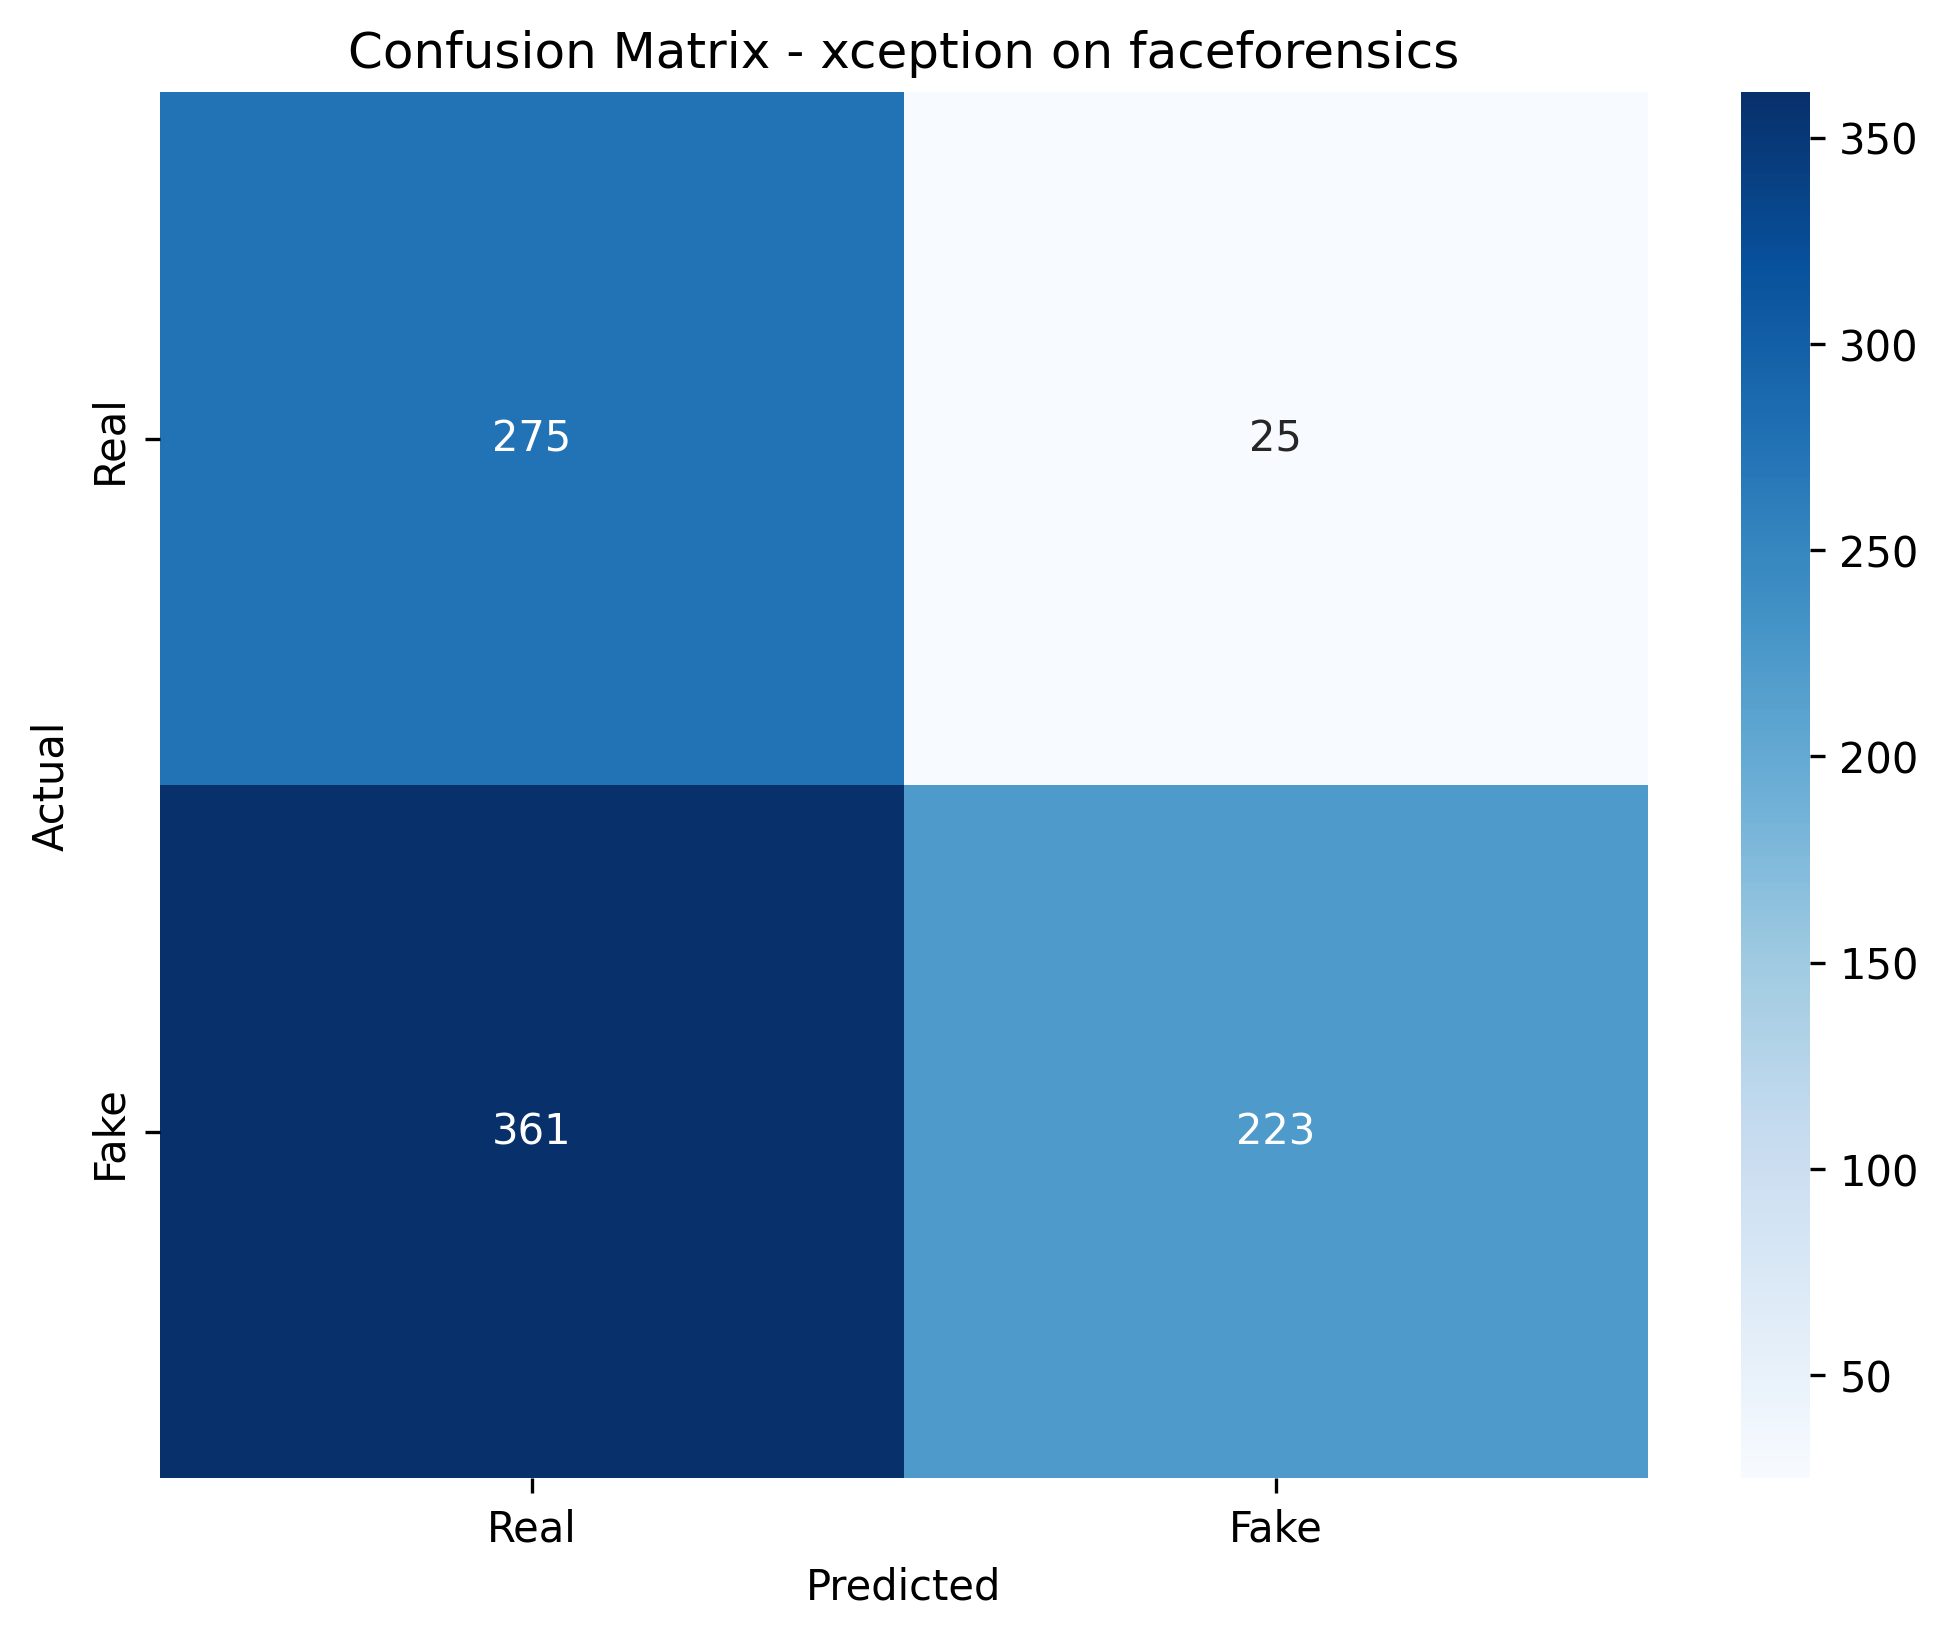
\includegraphics[width=0.24\textwidth]{figures/xception_faceforensics_confusion_matrix.png} \\
(a) EfficientNet-B0 & (b) XceptionNet \\
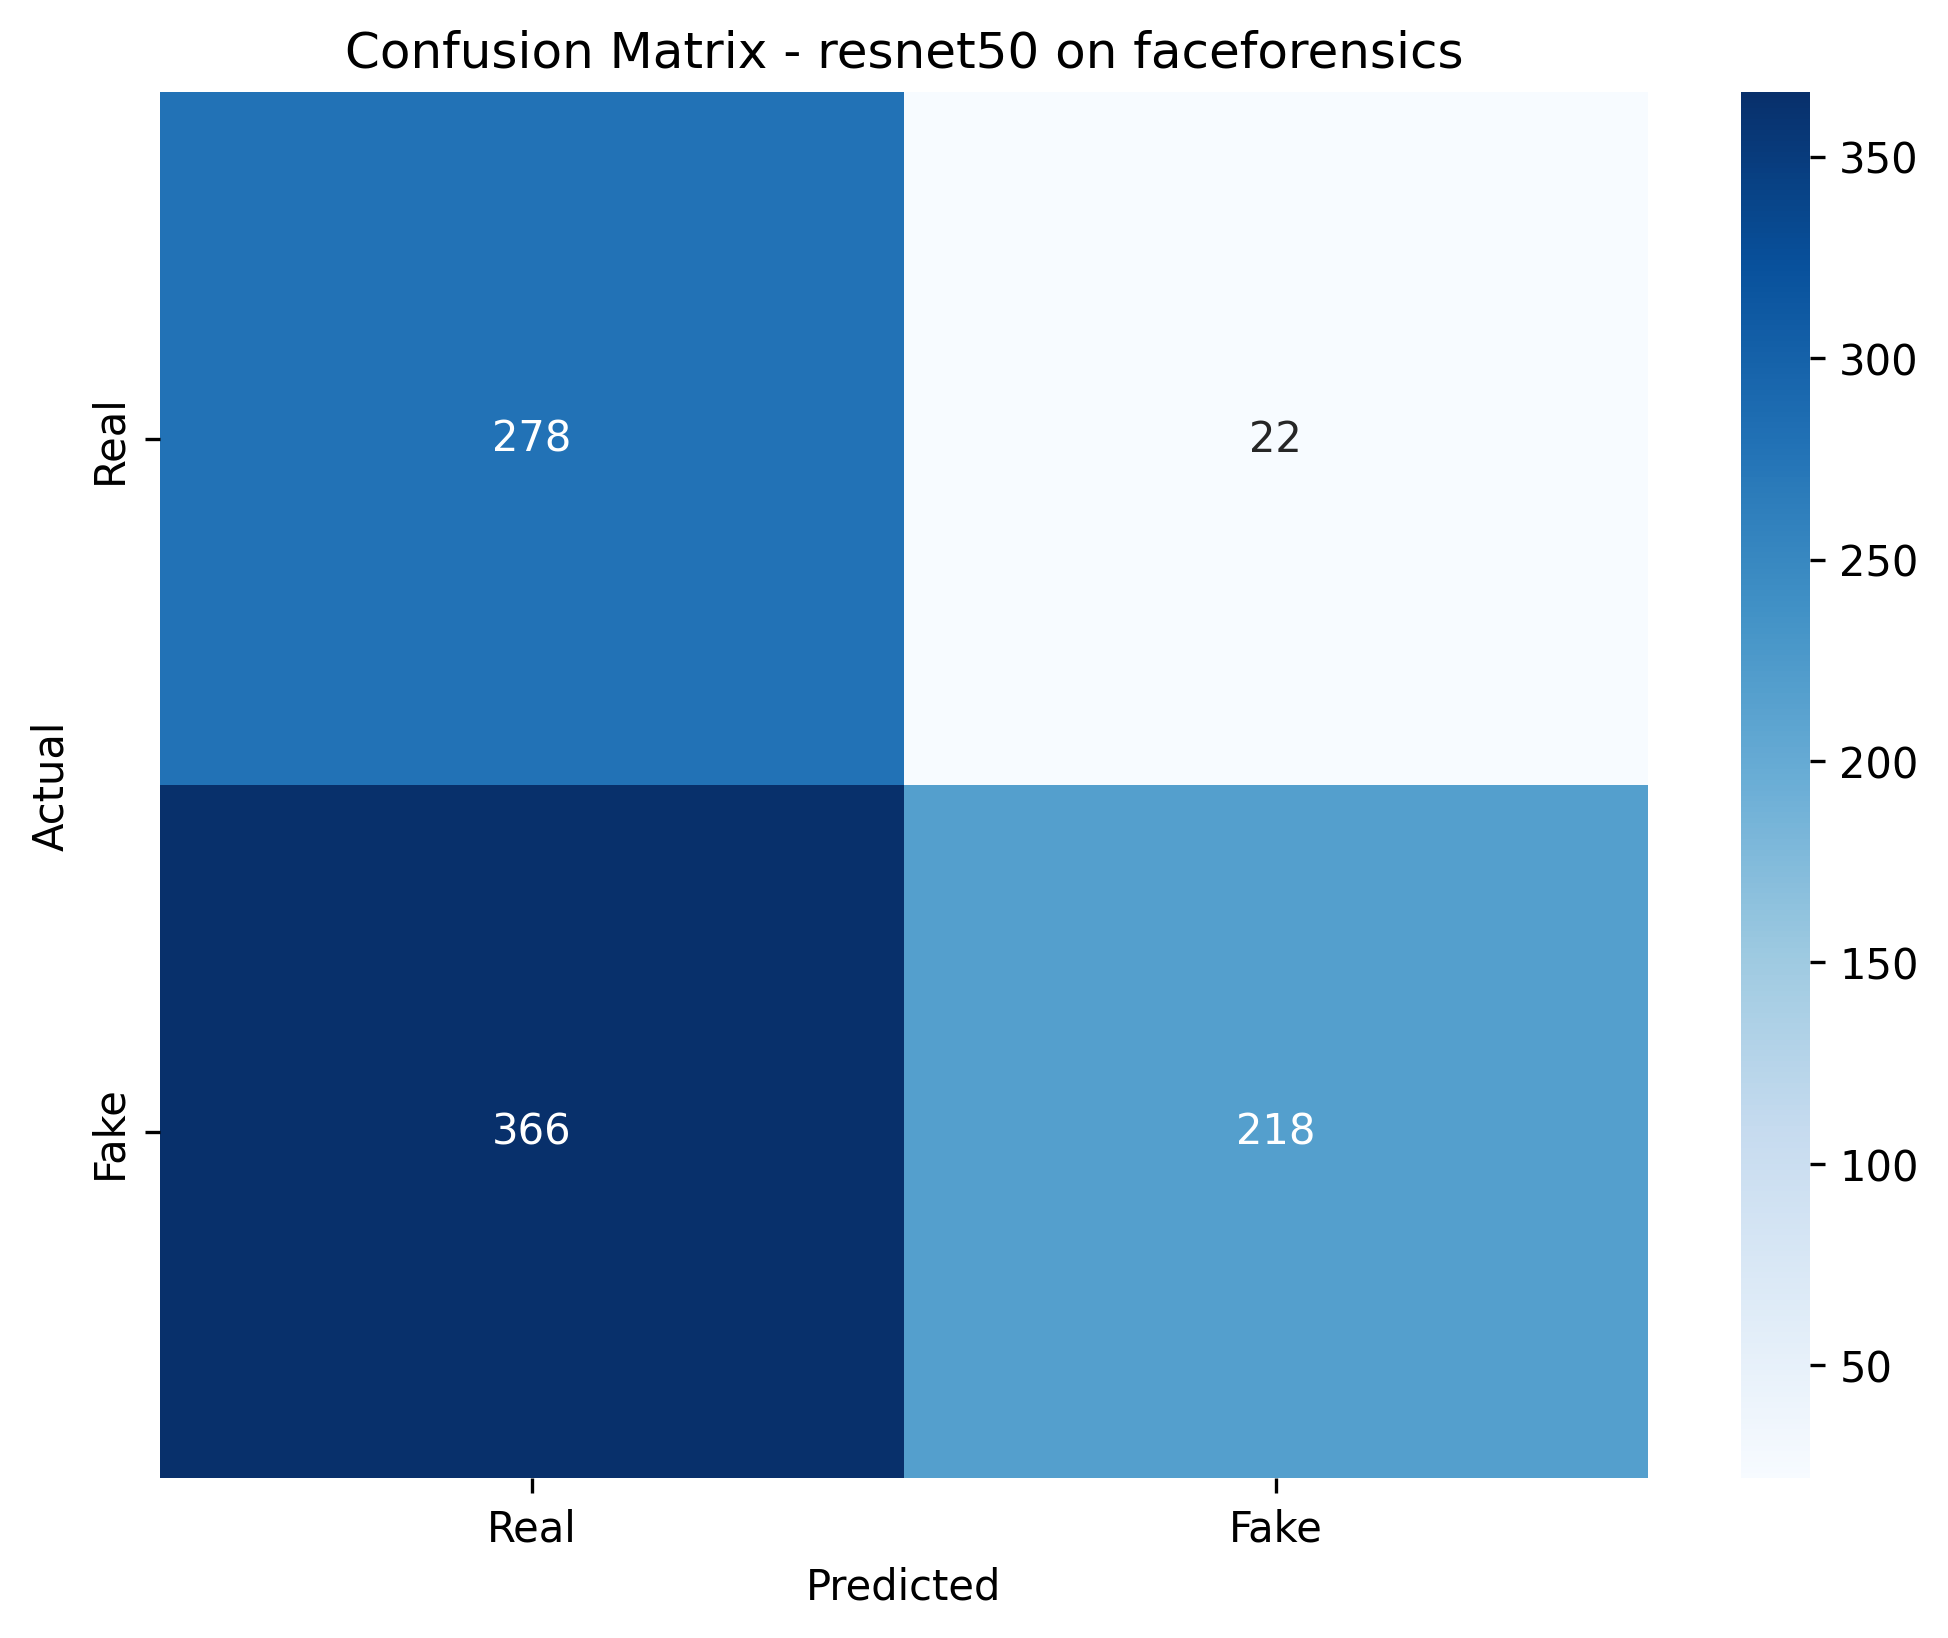
\includegraphics[width=0.24\textwidth]{figures/resnet50_faceforensics_confusion_matrix.png} &
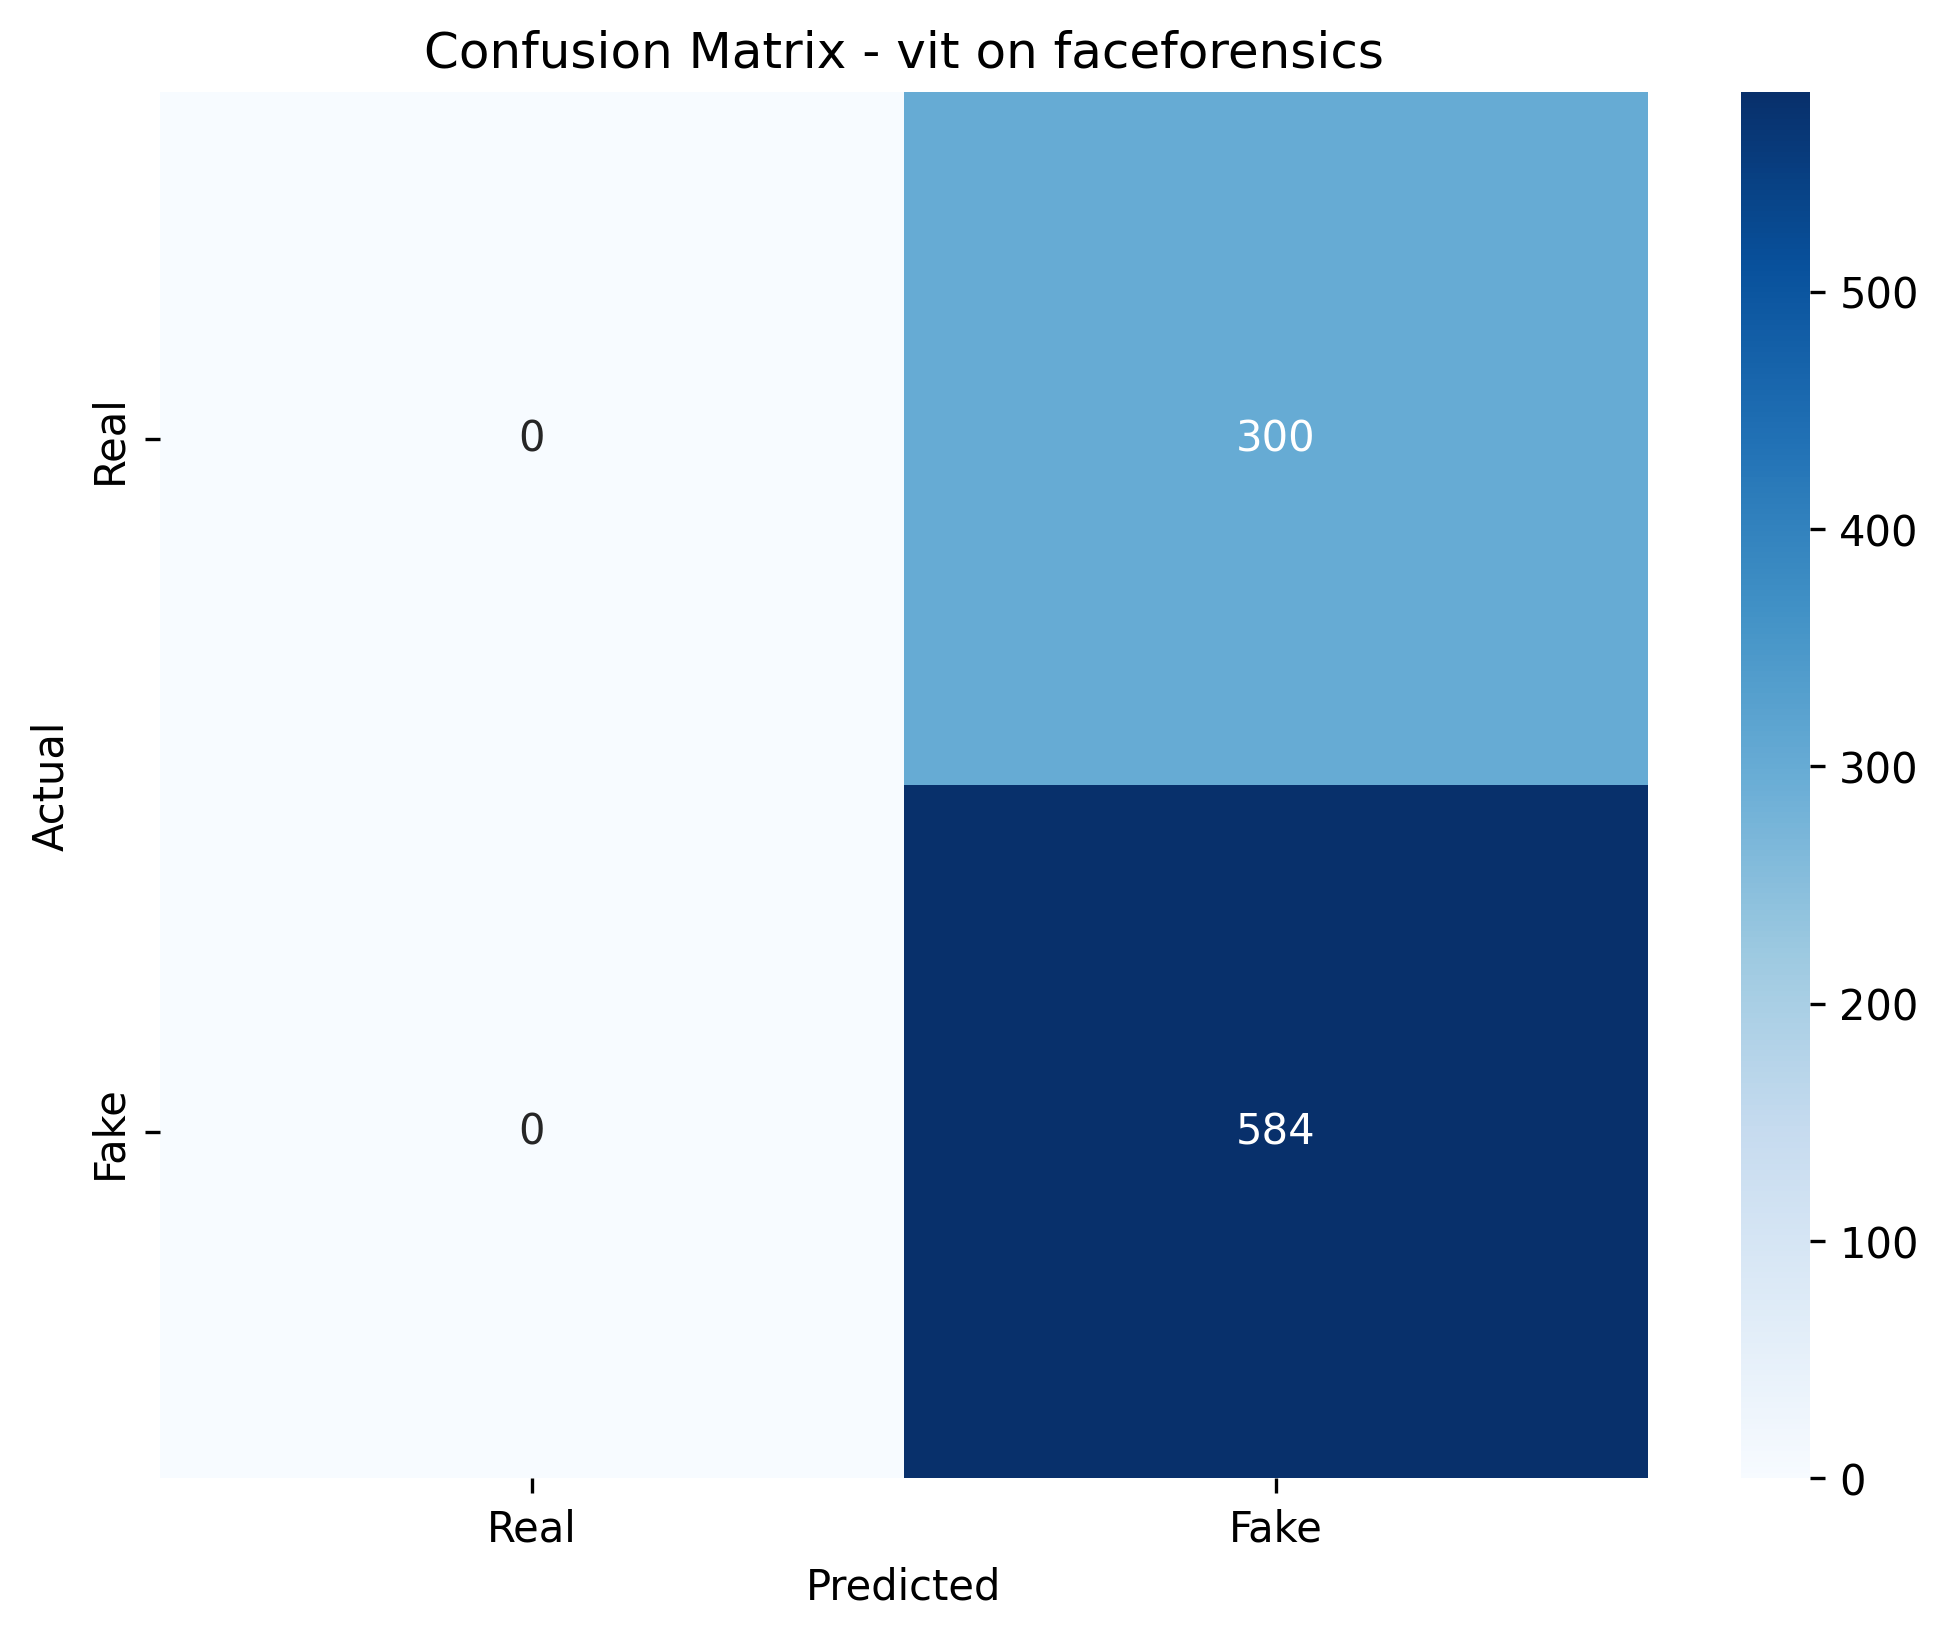
\includegraphics[width=0.24\textwidth]{figures/vit_faceforensics_confusion_matrix.png} \\
(c) ResNet50 & (d) Vision Transformer
\end{tabular}
\caption{Confusion matrices for cross-dataset evaluation (Celeb-DF trained models tested on FaceForensics++).}
\label{fig:confusion_ff}
\end{figure*}

Figure~\ref{fig:roc_ff} presents ROC curves for cross-dataset evaluation, demonstrating how model discriminative ability degrades when tested on FaceForensics++. The AUC values are substantially lower compared to in-distribution performance, with CNN-based models showing AUC values between 68-73\%, while Vision Transformer achieves 52.75\% AUC.

\begin{figure*}[!t]
\centering
\begin{tabular}{cc}
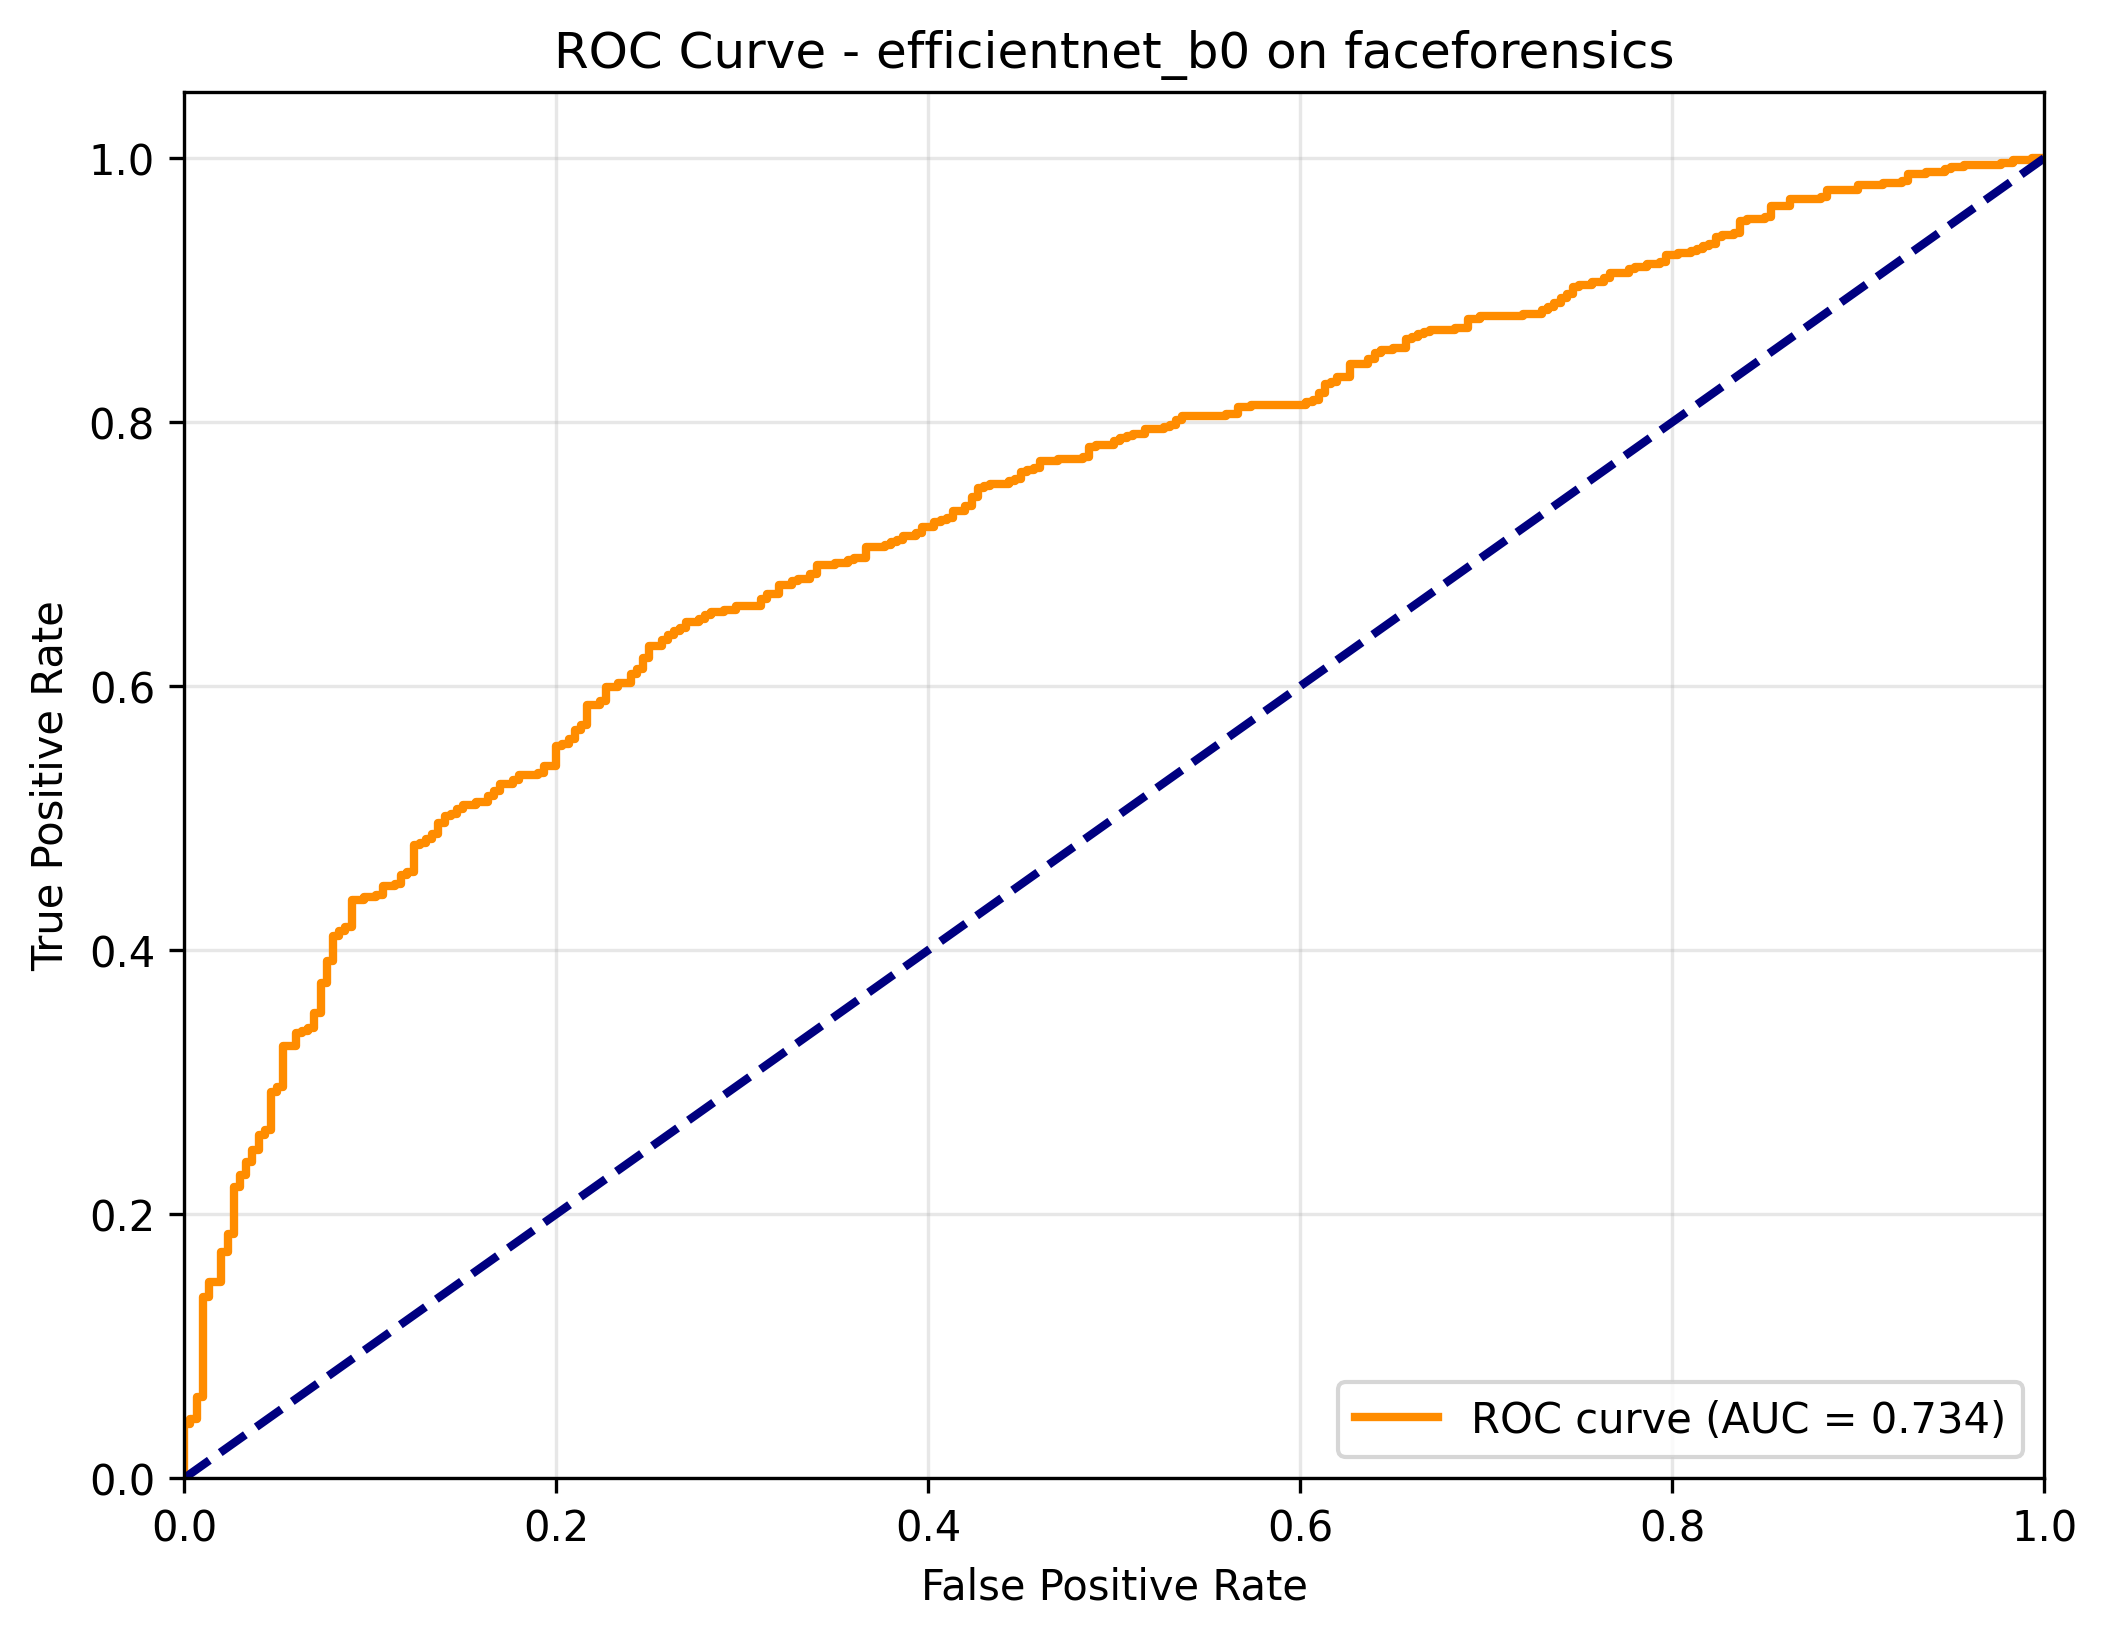
\includegraphics[width=0.24\textwidth]{figures/efficientnet_b0_faceforensics_roc_curve.png} &
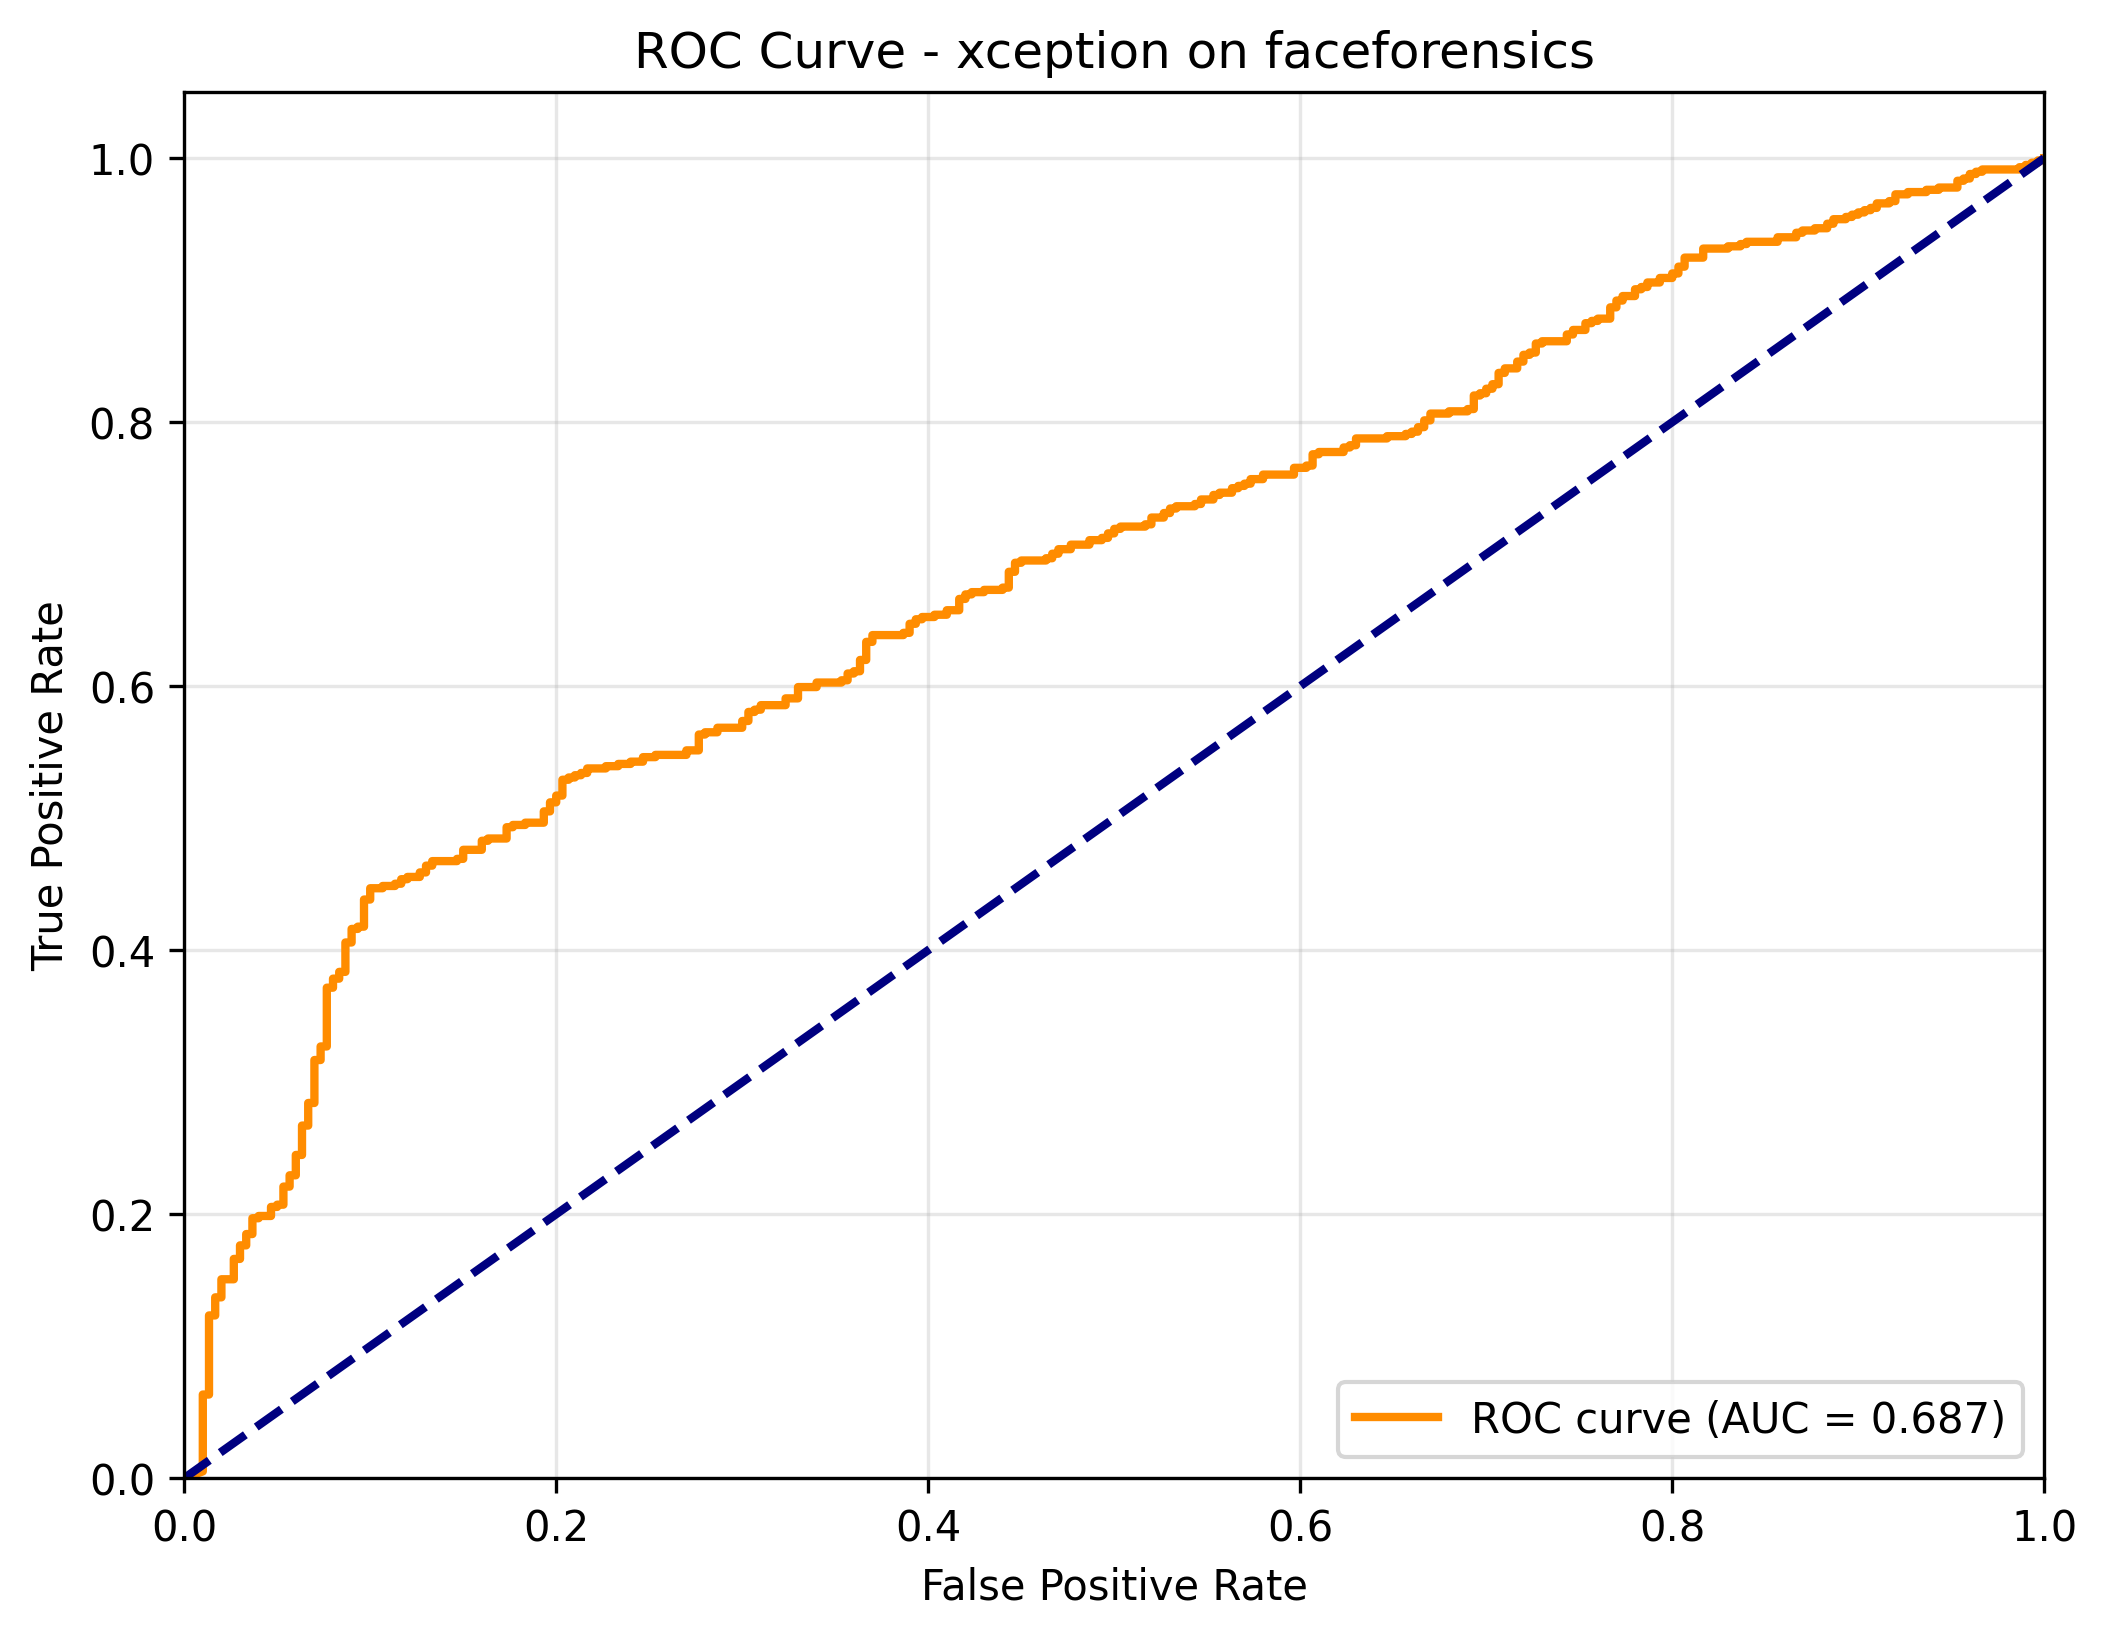
\includegraphics[width=0.24\textwidth]{figures/xception_faceforensics_roc_curve.png} \\
(a) EfficientNet-B0 & (b) XceptionNet \\
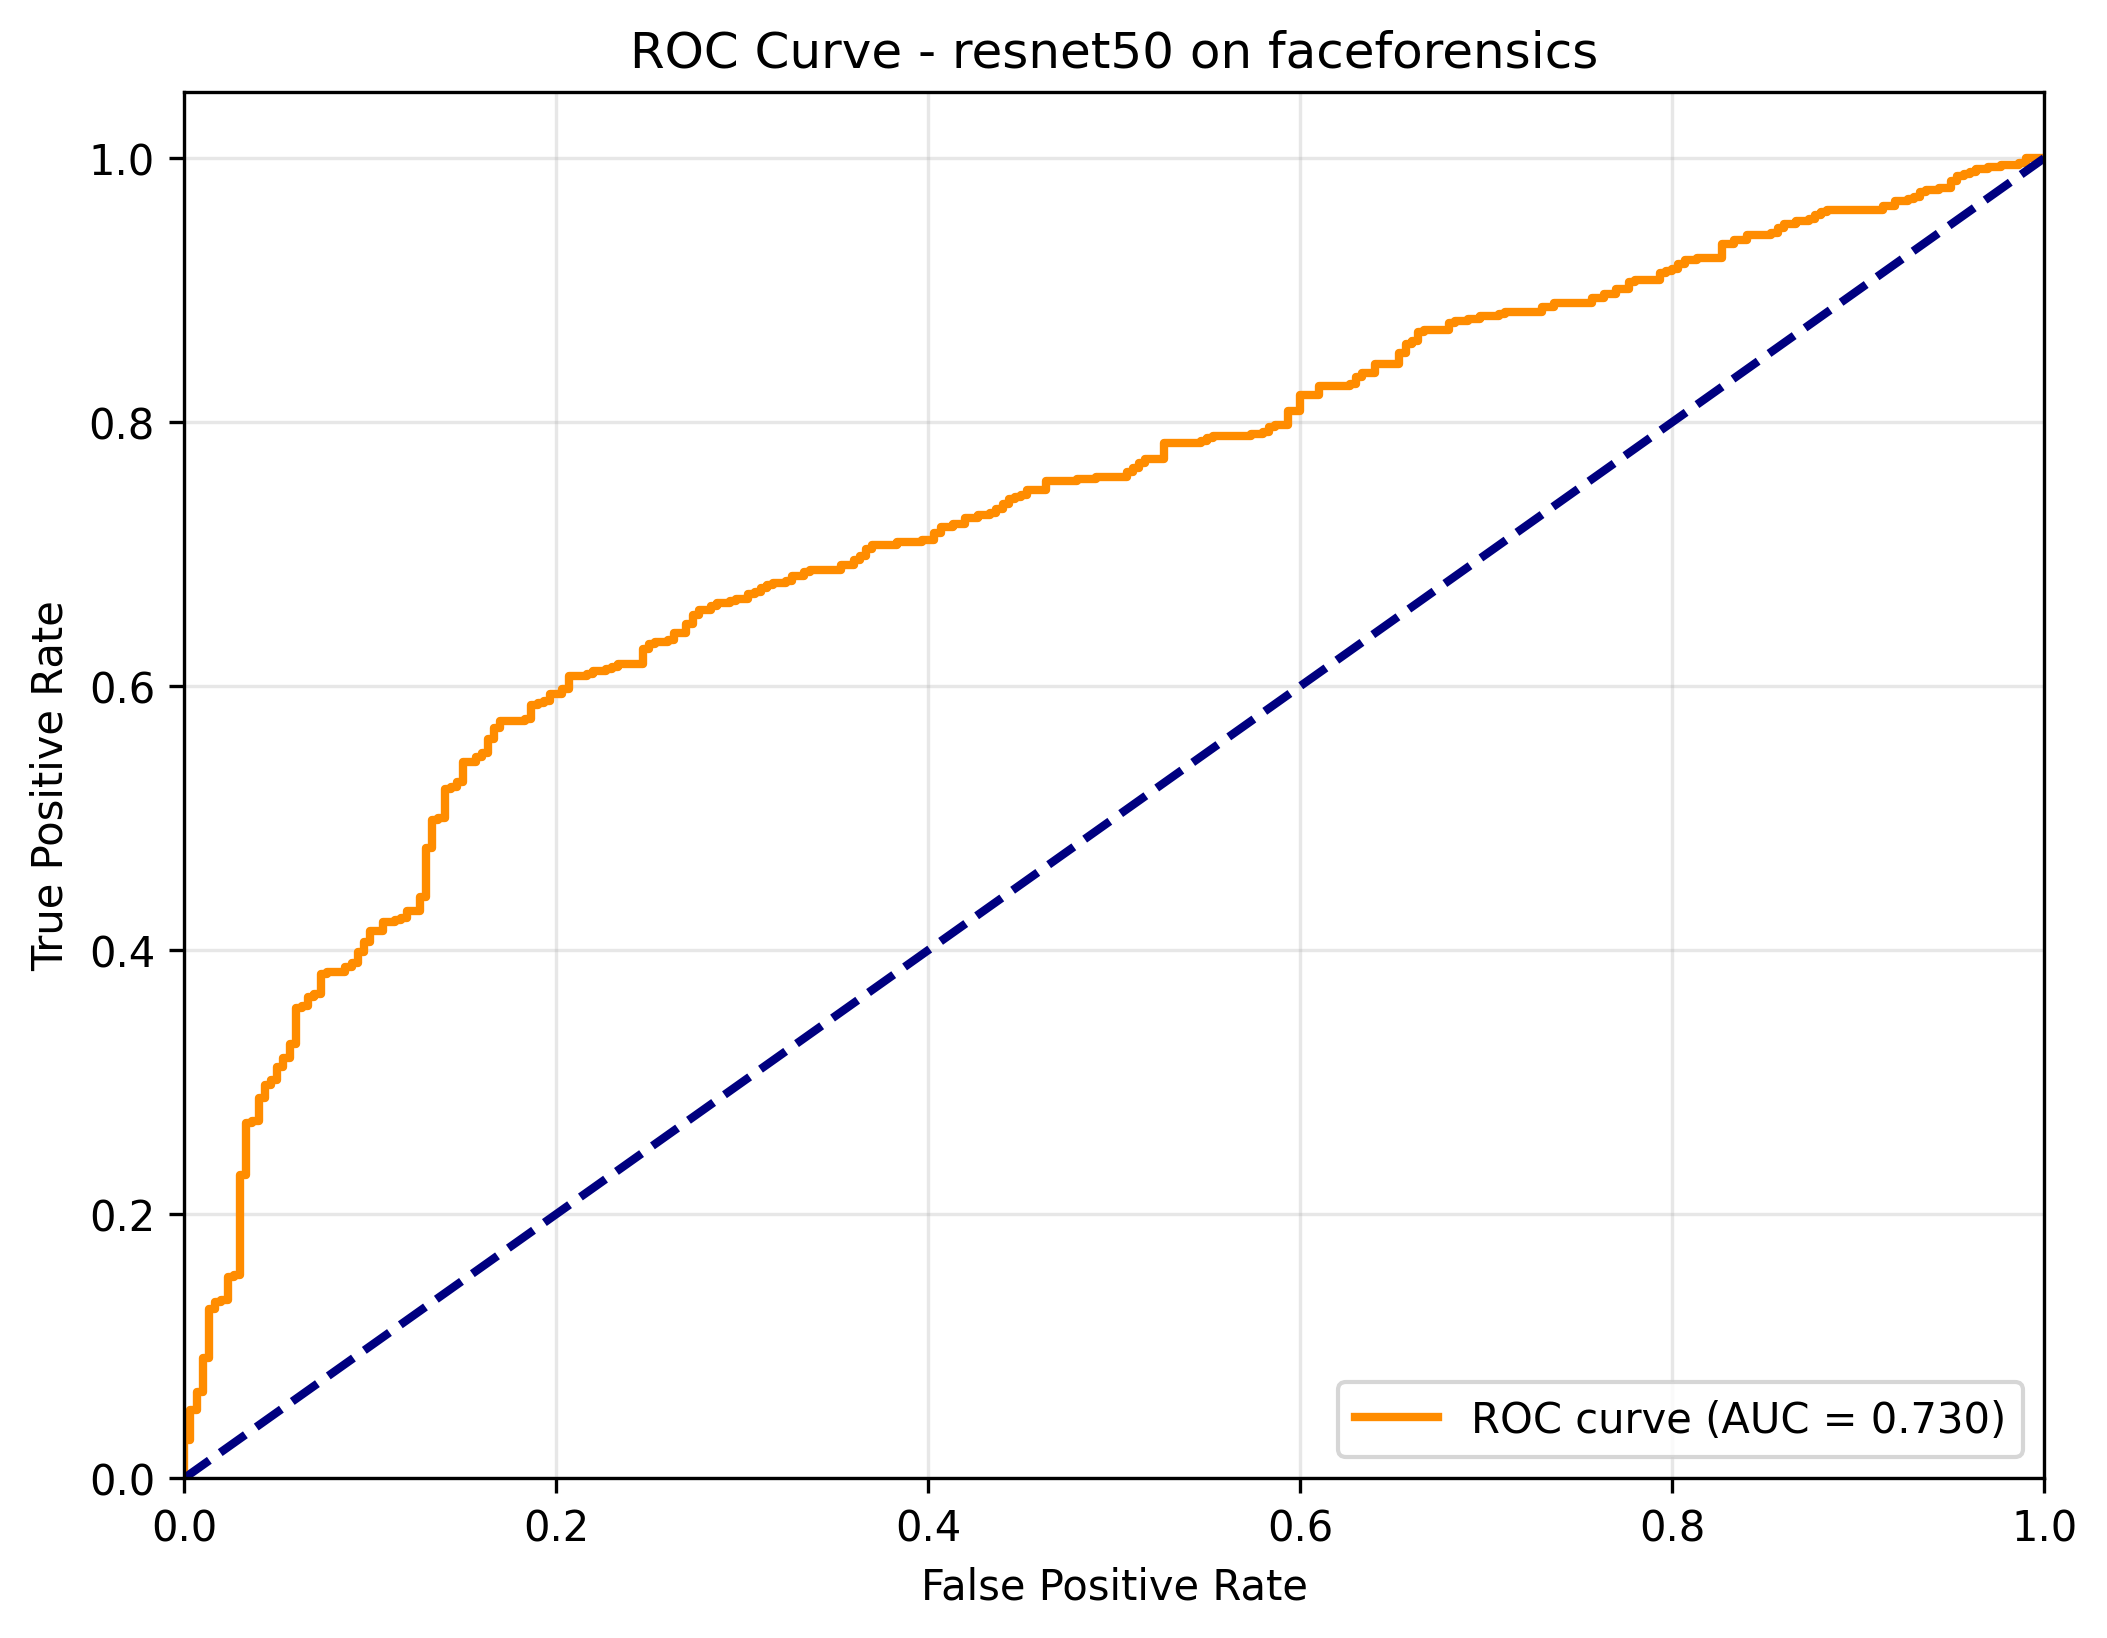
\includegraphics[width=0.24\textwidth]{figures/resnet50_faceforensics_roc_curve.png} &
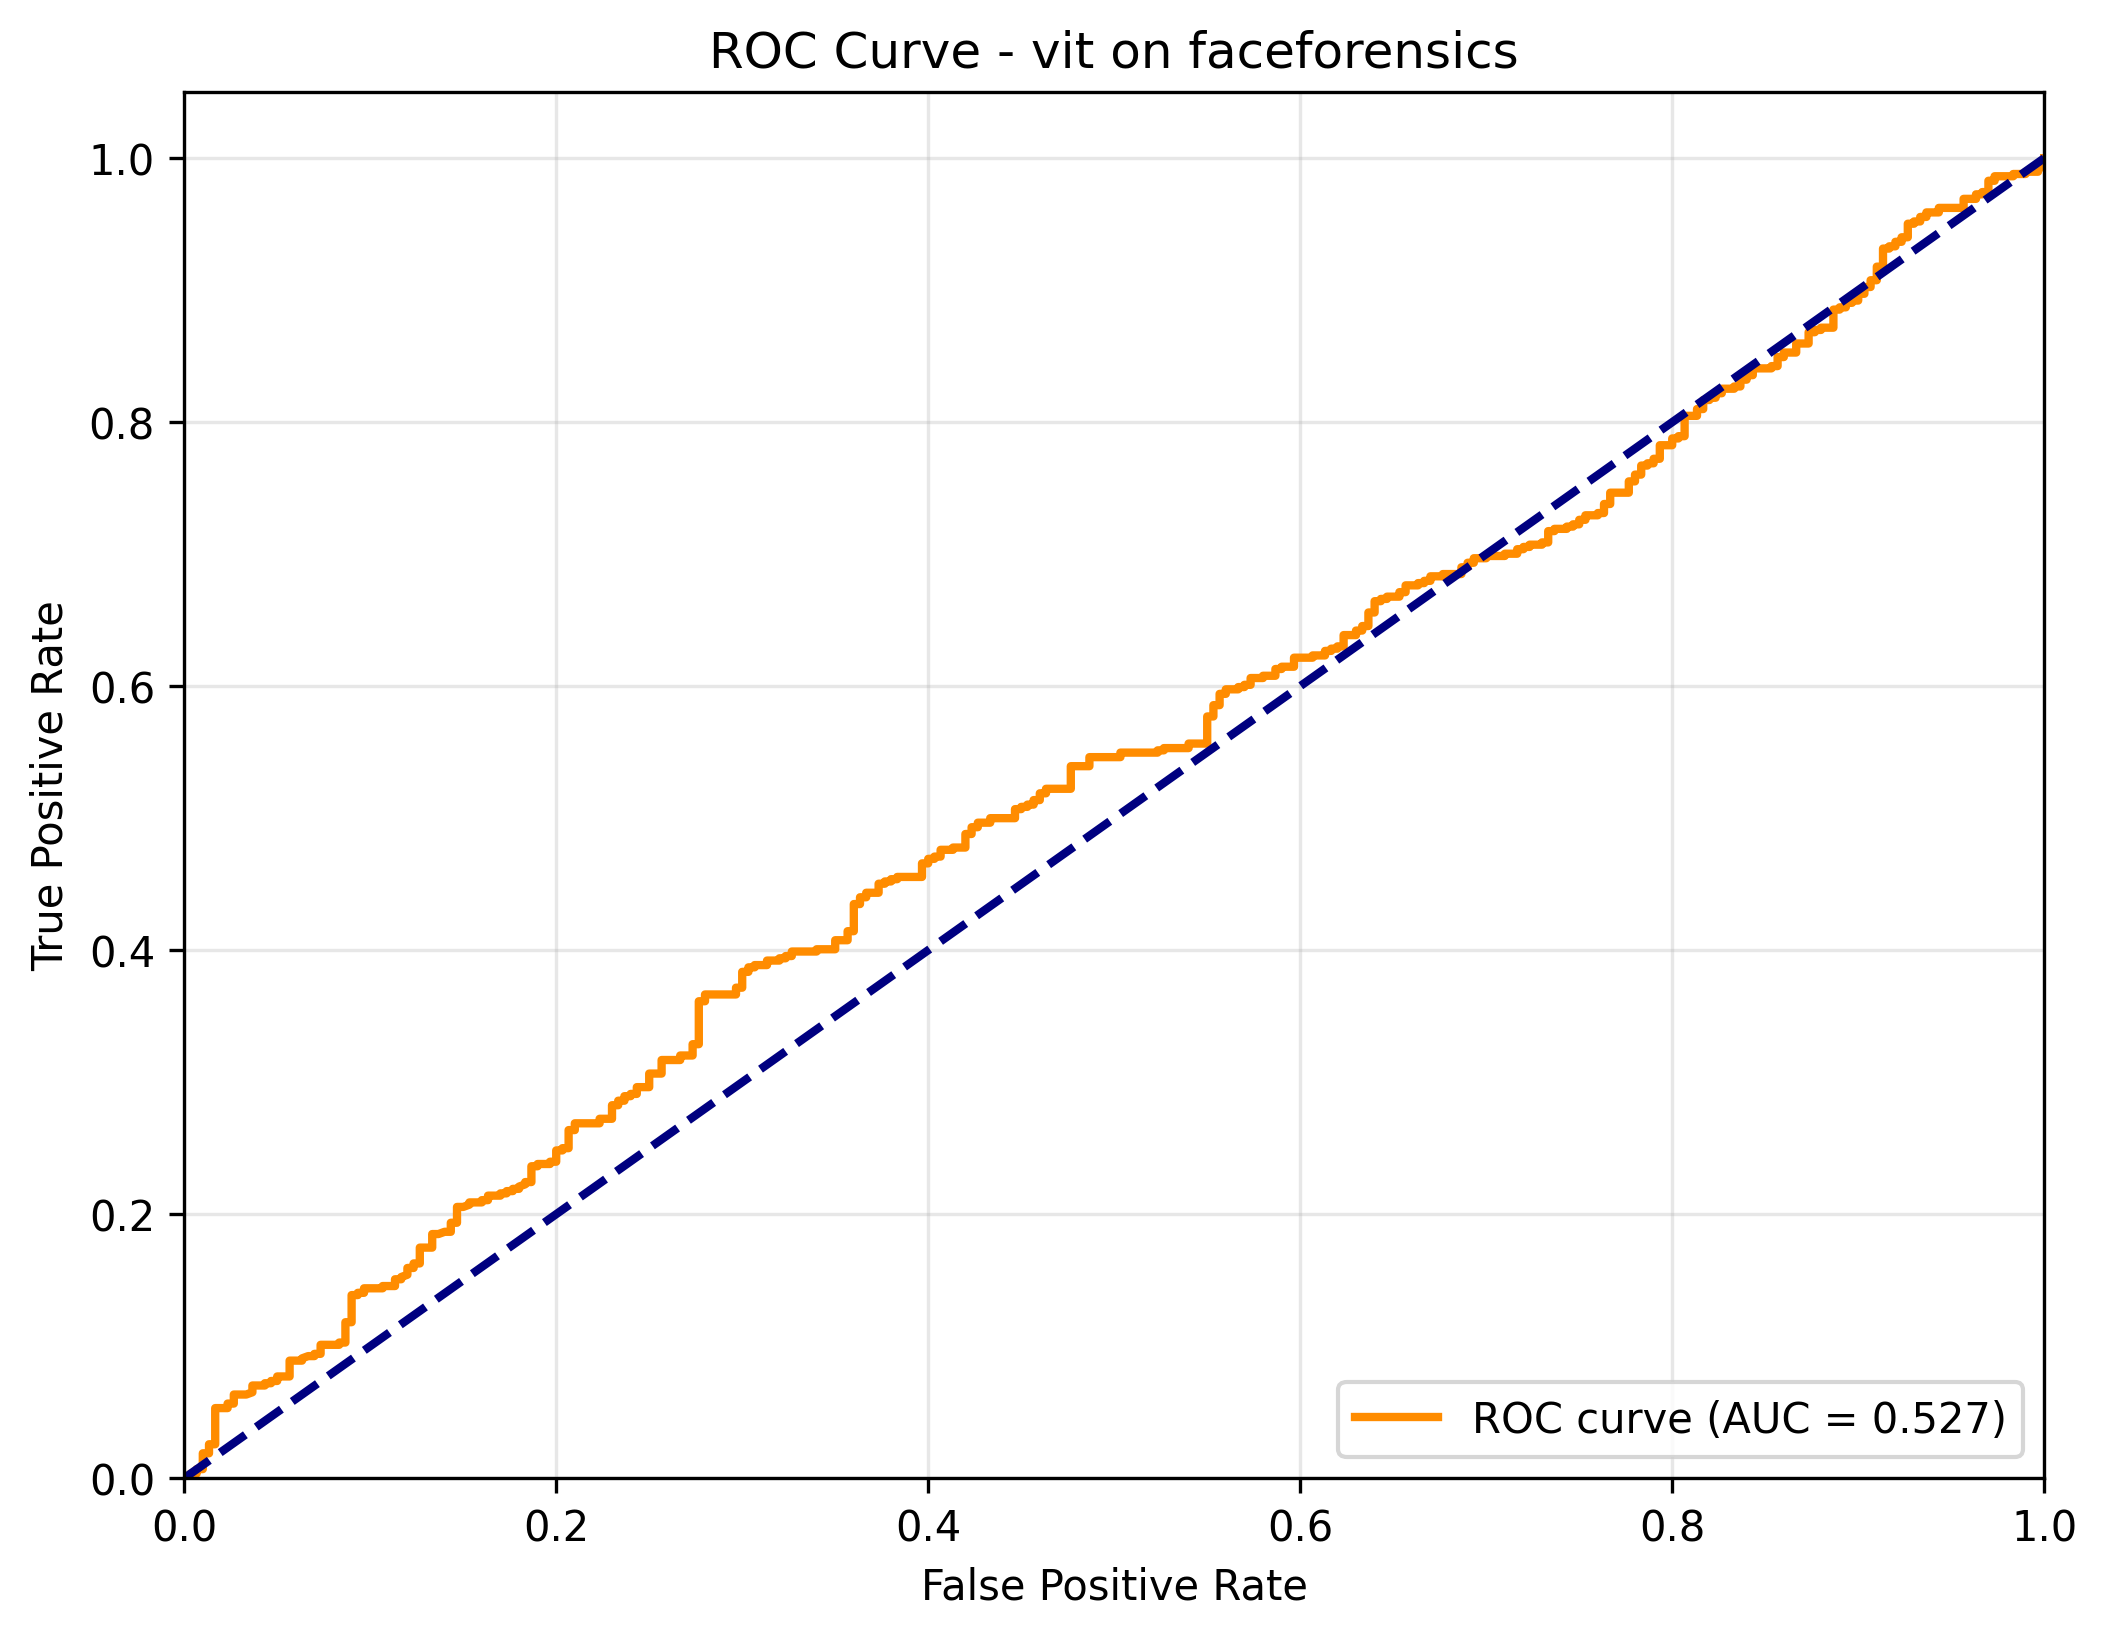
\includegraphics[width=0.24\textwidth]{figures/vit_faceforensics_roc_curve.png} \\
(c) ResNet50 & (d) Vision Transformer
\end{tabular}
\caption{ROC curves for cross-dataset evaluation (Celeb-DF trained models tested on FaceForensics++).}
\label{fig:roc_ff}
\end{figure*}

Figure~\ref{fig:pr_ff} shows precision-recall curves for cross-dataset evaluation, providing additional insights into model performance on the FaceForensics++ dataset. These curves reveal the trade-off between precision and recall when models encounter distribution shifts.

\begin{figure*}[!t]
\centering
\begin{tabular}{cc}
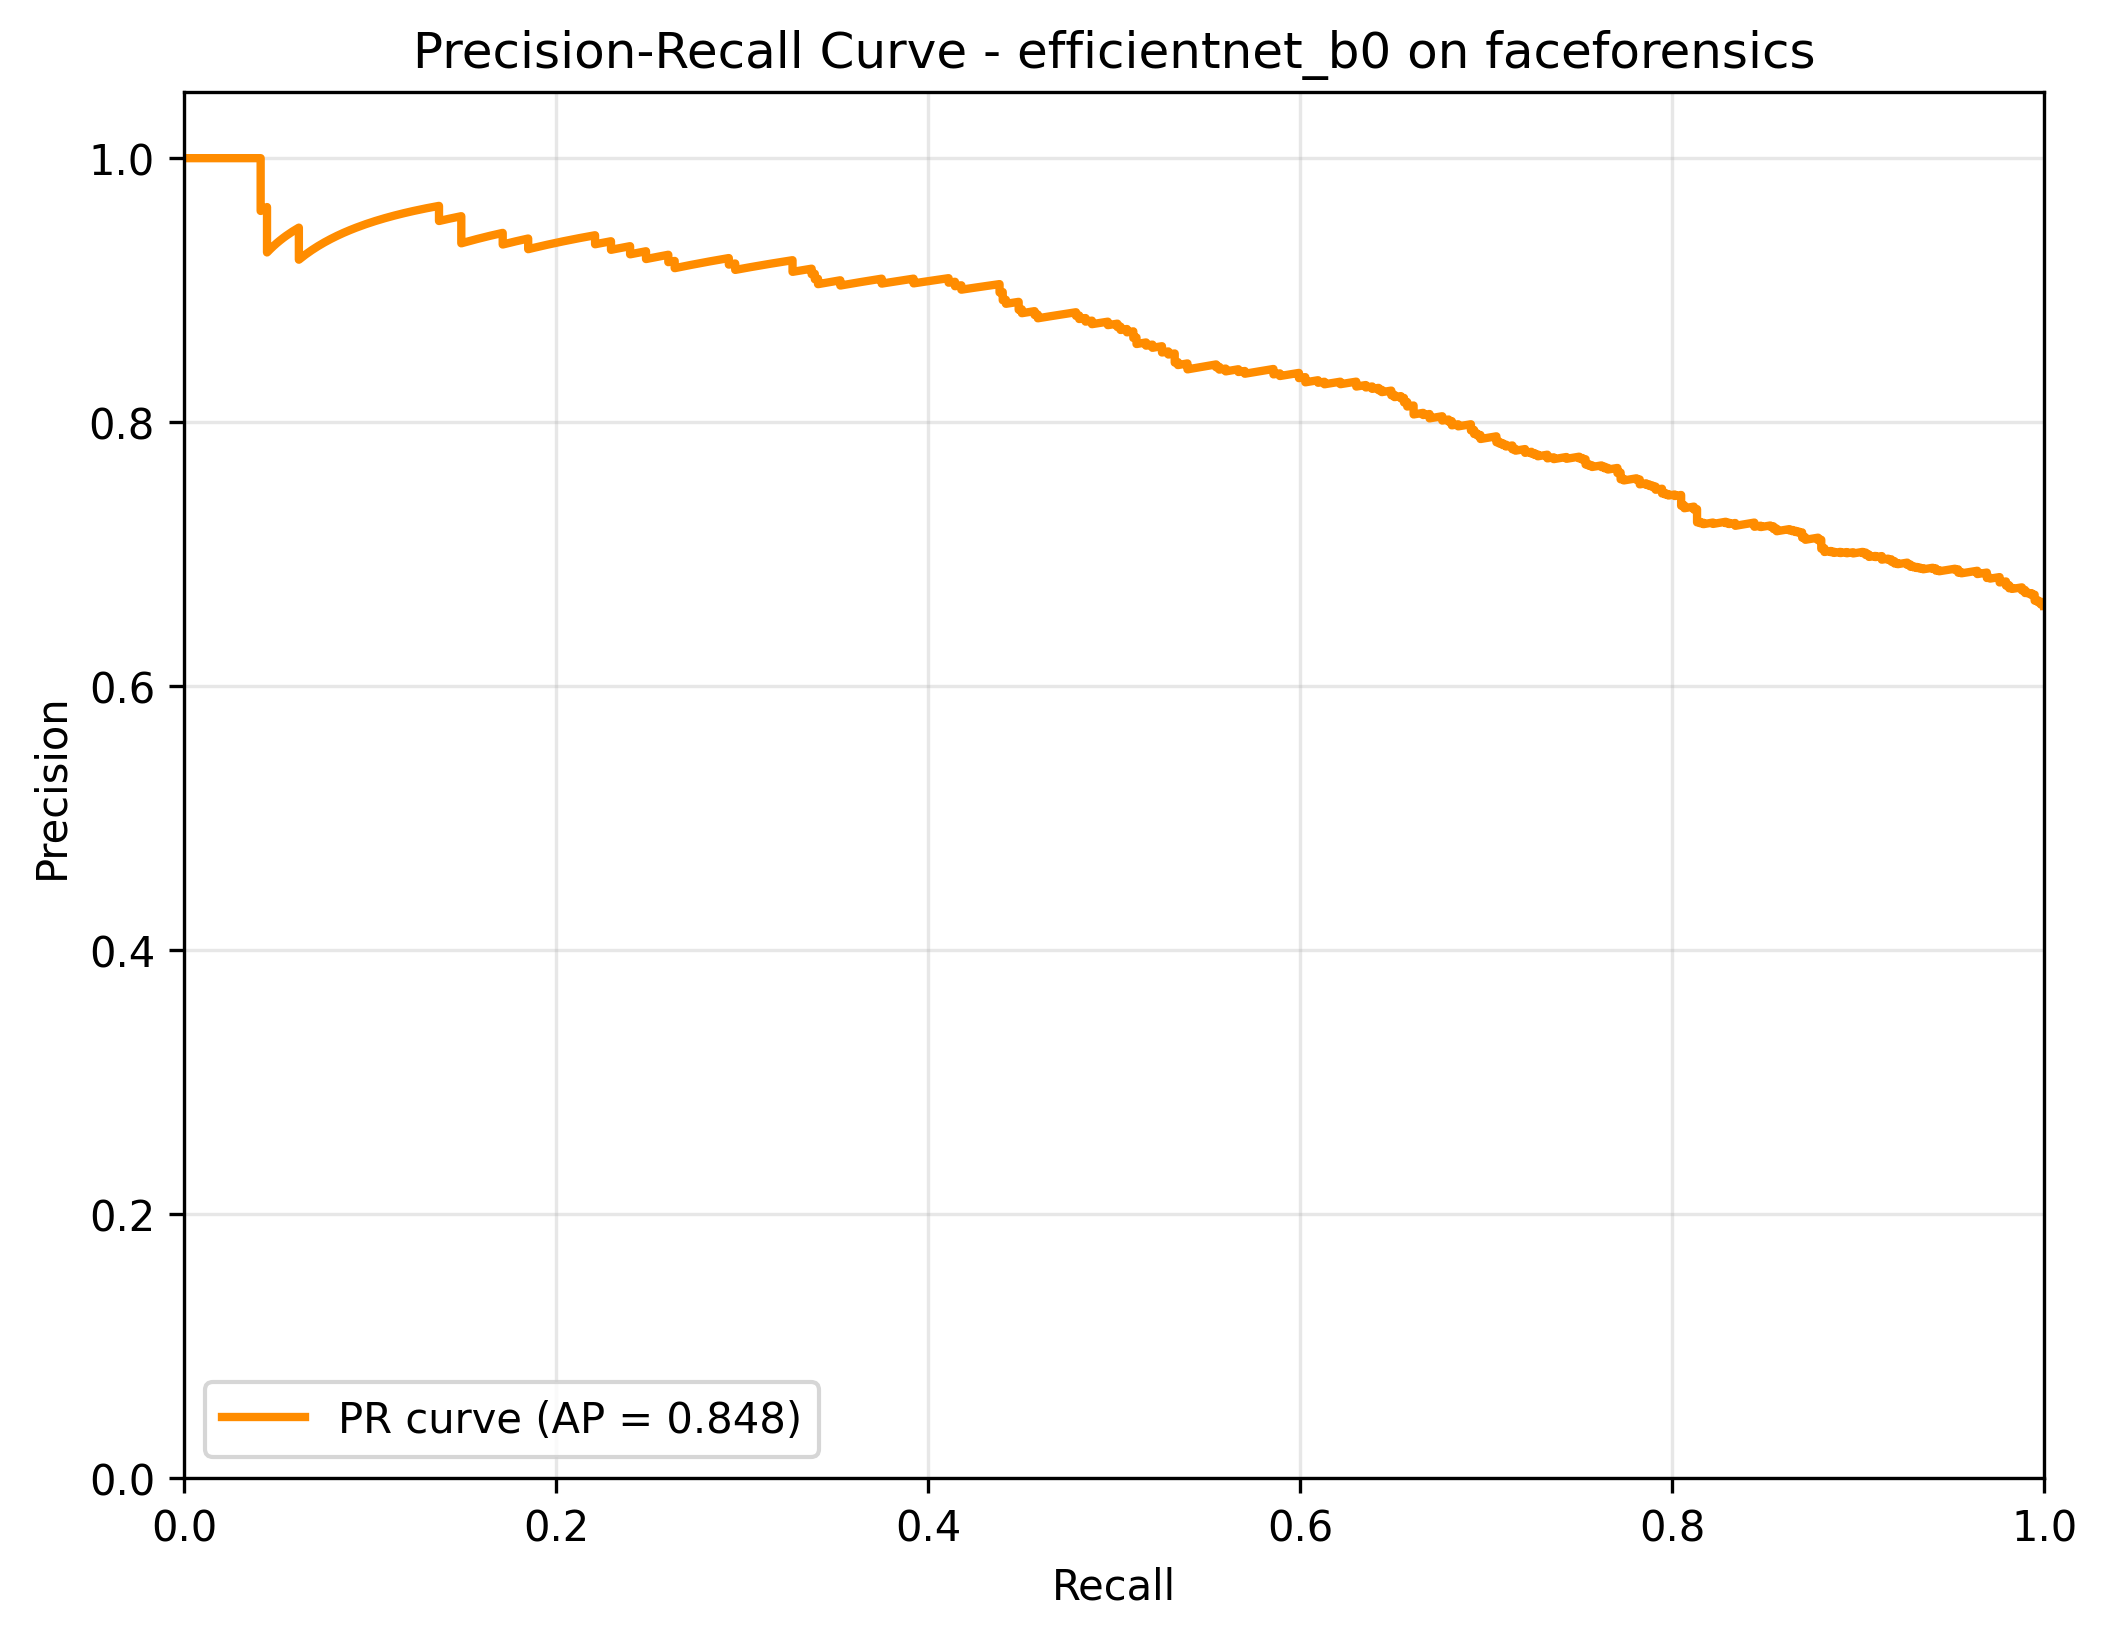
\includegraphics[width=0.24\textwidth]{figures/efficientnet_b0_faceforensics_precision_recall_curve.png} &
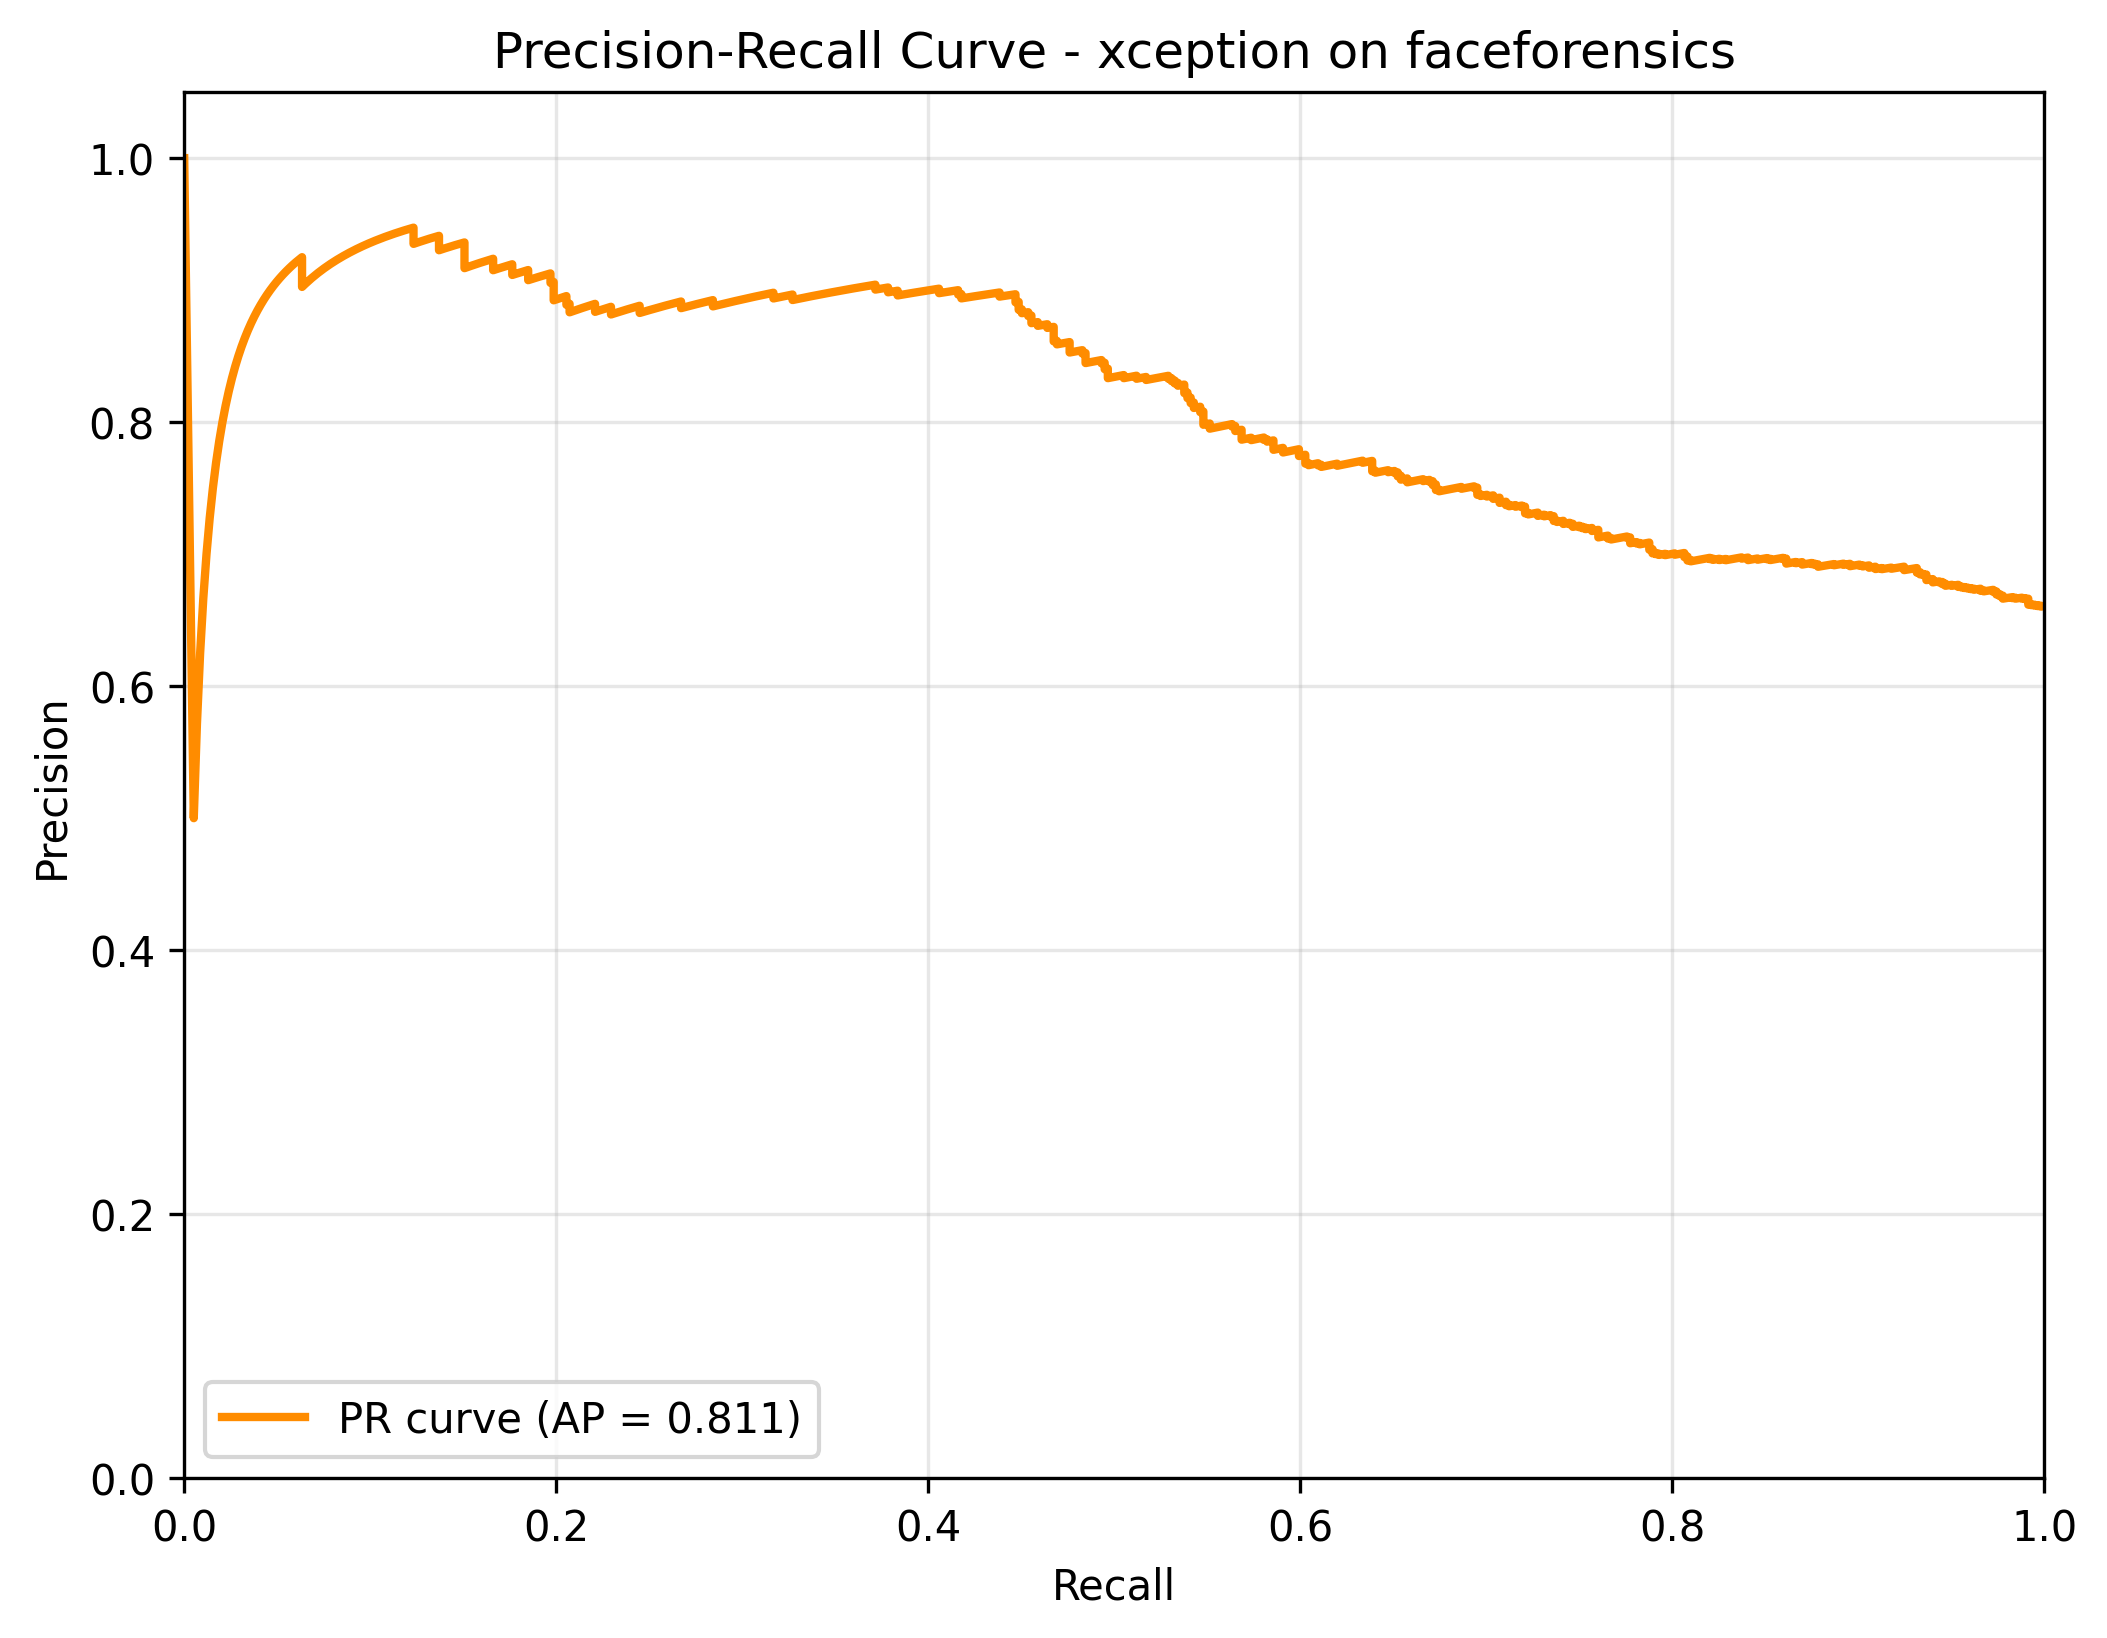
\includegraphics[width=0.24\textwidth]{figures/xception_faceforensics_precision_recall_curve.png} \\
(a) EfficientNet-B0 & (b) XceptionNet \\
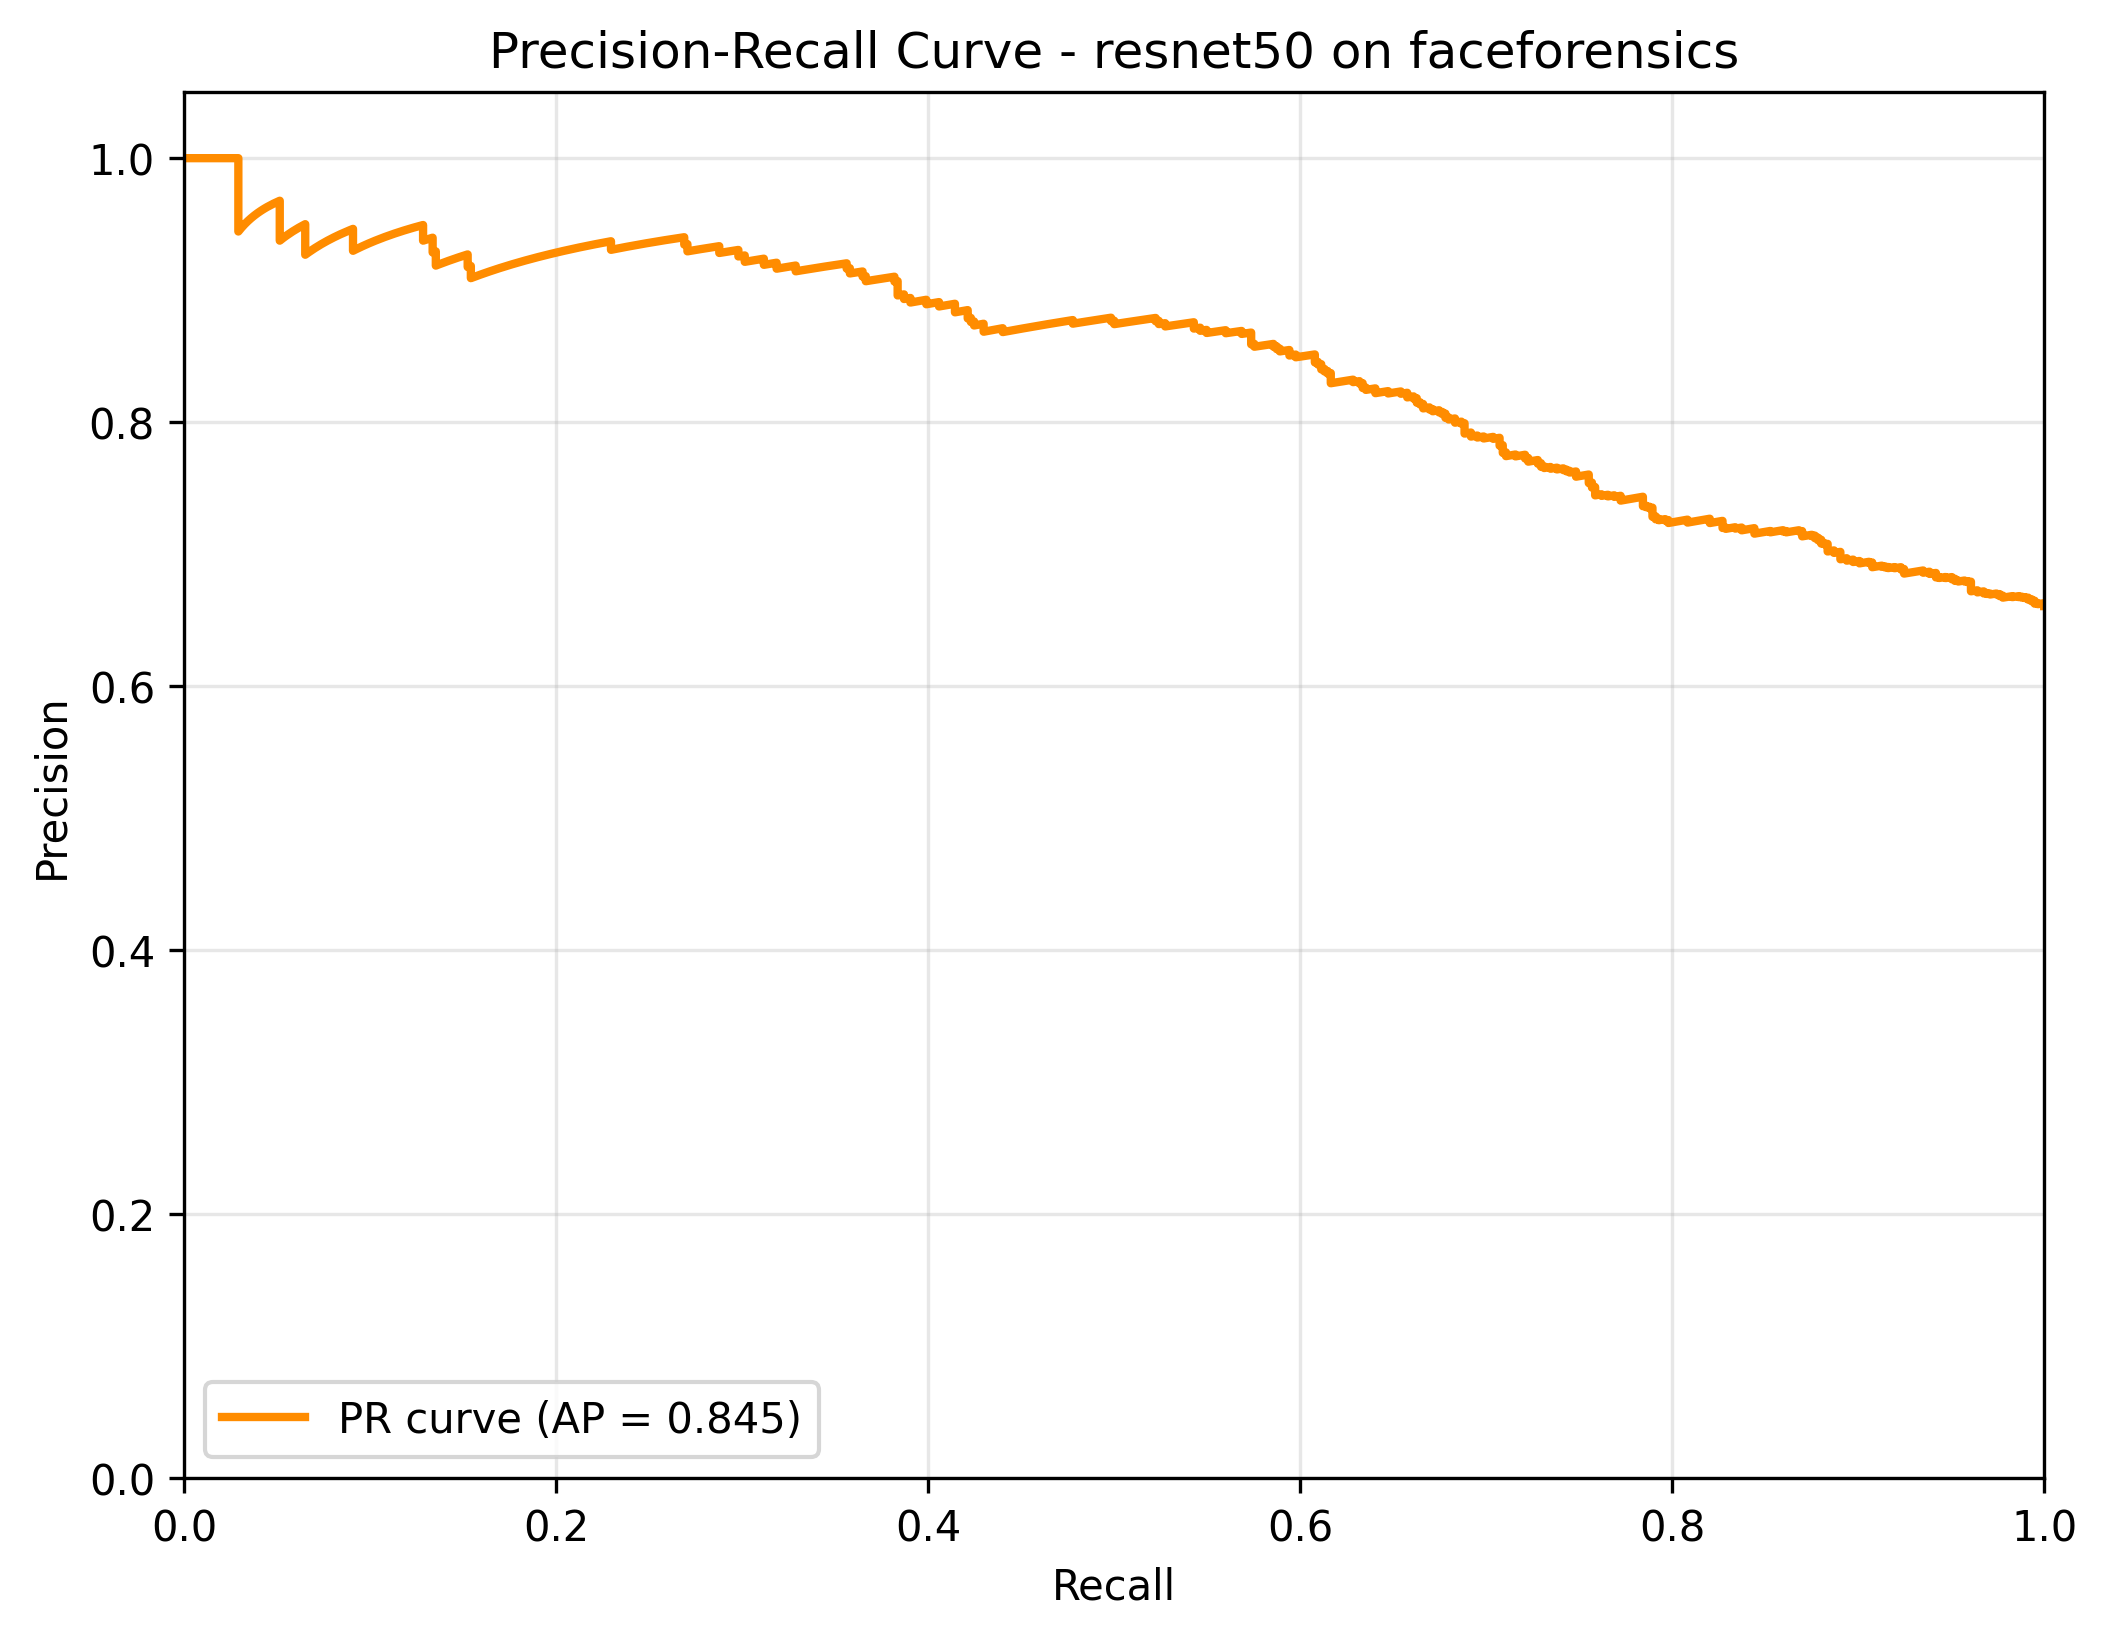
\includegraphics[width=0.24\textwidth]{figures/resnet50_faceforensics_precision_recall_curve.png} &
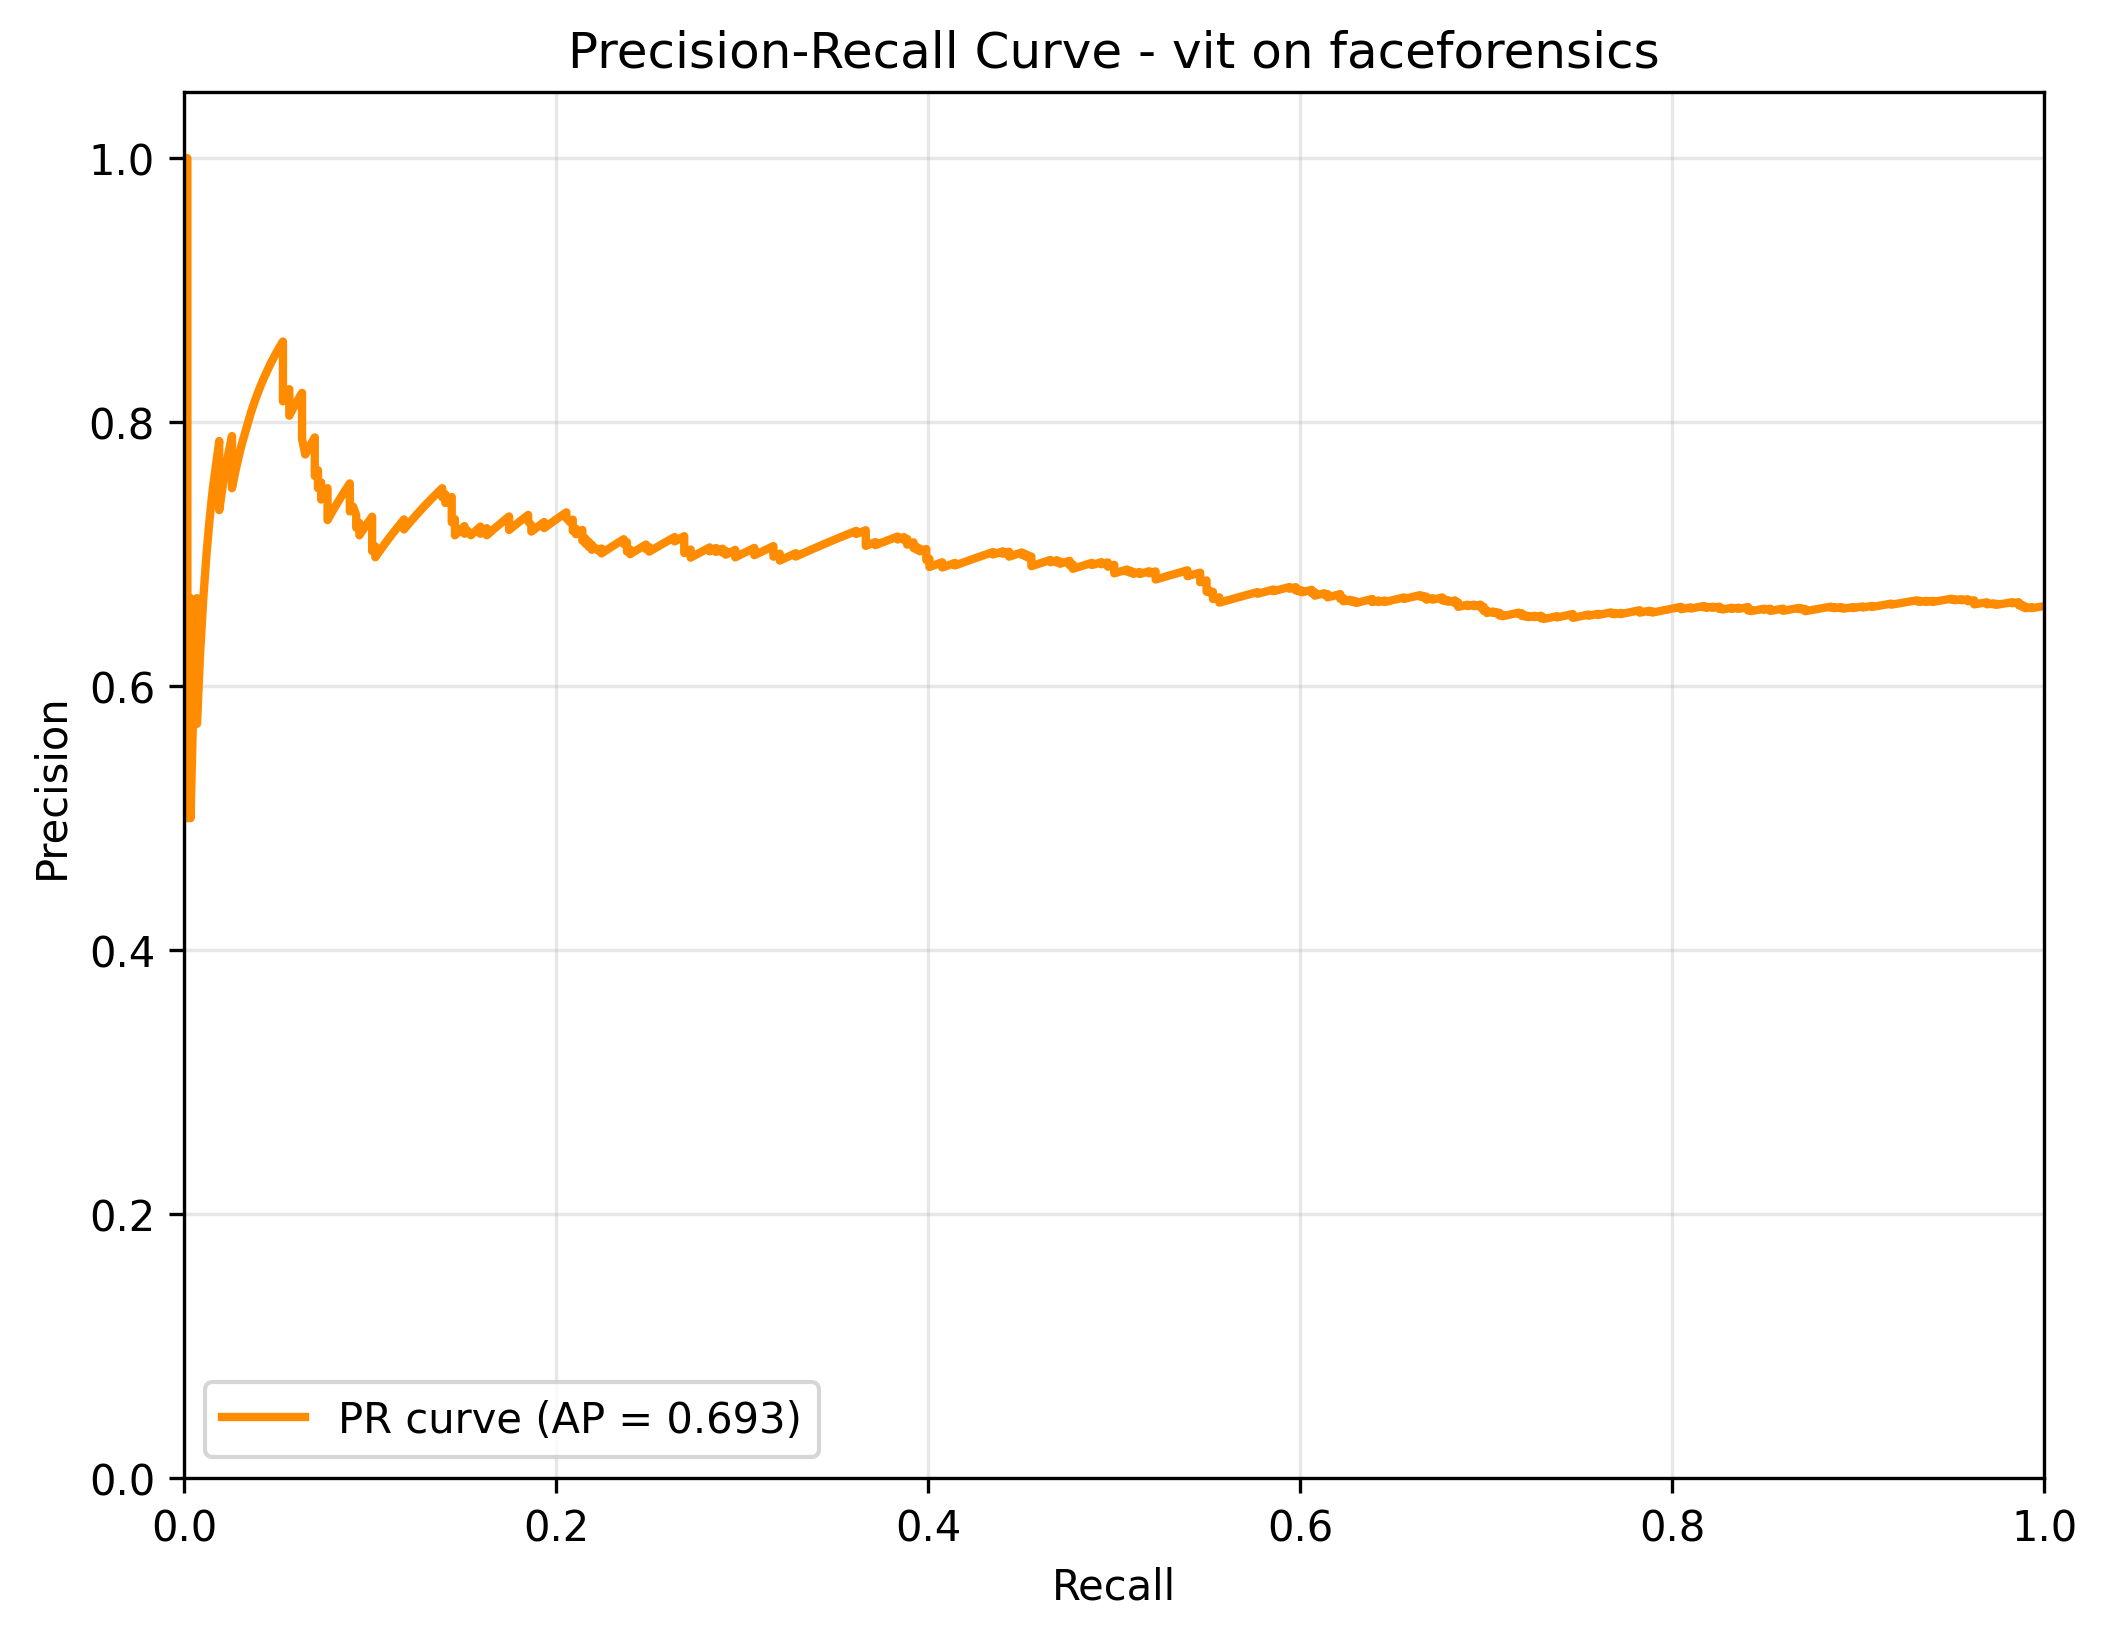
\includegraphics[width=0.24\textwidth]{figures/vit_faceforensics_precision_recall_curve.png} \\
(c) ResNet50 & (d) Vision Transformer
\end{tabular}
\caption{Precision-Recall curves for cross-dataset evaluation (Celeb-DF trained models tested on FaceForensics++).}
\label{fig:pr_ff}
\end{figure*}

\subsection{Interpretability Analysis}
Through Grad-CAM visualization analysis, we observe that all four architectures consistently focus their attention on facial regions when making classification decisions. This finding indicates that models learn to identify facial features and manipulation artifacts rather than relying on background information or dataset-specific biases. 

Figure~\ref{fig:gradcam} presents representative Grad-CAM visualizations, showing attention heatmaps overlaid on sample images. The attention patterns exhibit subtle variations across architectures. EfficientNet-B0 and XceptionNet demonstrate more localized, concentrated attention regions, suggesting they identify specific facial features or artifacts. In contrast, ResNet50 and Vision Transformer exhibit more distributed attention patterns, potentially capturing broader contextual information across facial regions.

\begin{figure*}[!t]
\centering
\begin{tabular}{cc}
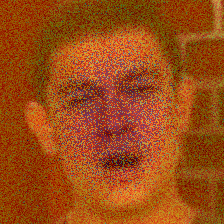
\includegraphics[width=0.18\textwidth]{figures/efficientnet_b0_gradcam_fake.png} &
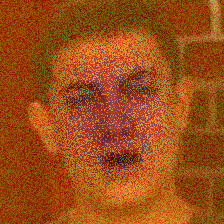
\includegraphics[width=0.18\textwidth]{figures/efficientnet_b0_gradcam_real.png} \\
(a) EfficientNet-B0: Fake & (b) EfficientNet-B0: Real \\
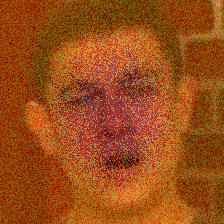
\includegraphics[width=0.18\textwidth]{figures/xception_gradcam_fake.png} &
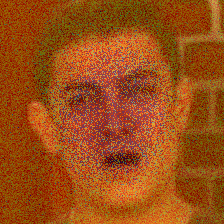
\includegraphics[width=0.18\textwidth]{figures/xception_gradcam_real.png} \\
(c) XceptionNet: Fake & (d) XceptionNet: Real \\
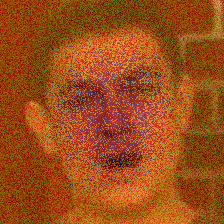
\includegraphics[width=0.18\textwidth]{figures/resnet50_gradcam_fake.png} &
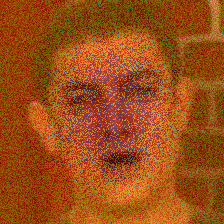
\includegraphics[width=0.18\textwidth]{figures/resnet50_gradcam_real.png} \\
(e) ResNet50: Fake & (f) ResNet50: Real \\
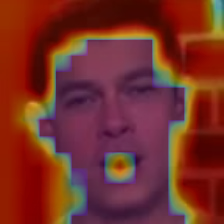
\includegraphics[width=0.18\textwidth]{figures/vit_gradcam_fake.png} &

\includegraphics[width=0.18\textwidth]{figures/vit_gradcam_real.png} \\
(g) Vision Transformer: Fake & (h) Vision Transformer: Real
\end{tabular}
\caption{Grad-CAM visualizations showing model attention patterns across all four architectures. Red regions indicate high importance for classification decisions.}
\label{fig:gradcam}
\end{figure*}

These visualizations provide valuable insights into model behavior, confirming that all architectures learn meaningful facial feature representations rather than exploiting irrelevant correlations. The consistent focus on facial regions across different architectures suggests that this represents a fundamental characteristic of effective deepfake detection.

\subsection{Discussion}
Our experimental findings reveal several important patterns:

\begin{enumerate}
    \item \textbf{In-Distribution Superiority of CNNs:} Convolutional architectures demonstrate exceptional performance when evaluated on data from the same distribution as training, with all three CNN models achieving accuracy above 98\%. This suggests that convolutional inductive biases are well-suited for learning dataset-specific patterns in deepfake detection.

    \item \textbf{Generalization Limitations:} The substantial performance degradation observed in cross-dataset evaluation indicates that current deepfake detection systems remain vulnerable to distribution shifts. This finding highlights the ongoing challenge of developing truly robust detection systems that generalize across diverse generation methods and data sources.

    \item \textbf{Transformer Generalization Advantage:} Despite achieving lower in-distribution accuracy, the Vision Transformer exhibits superior cross-dataset performance, suggesting that attention-based mechanisms may facilitate learning of more transferable feature representations. This observation warrants further investigation into hybrid architectures combining convolutional and attention-based processing.

    \item \textbf{Architecture Trade-offs:} Our results reveal a fundamental trade-off between in-distribution accuracy and cross-dataset generalization. CNN-based models excel at the former, while transformer-based models show promise for the latter. This suggests that practical deployment may require ensemble approaches or domain adaptation techniques.
\end{enumerate}

\section{Conclusion and Future Scope}
This investigation presents a systematic comparison of four deep learning architectures for deepfake detection, revealing important insights regarding their relative strengths and limitations. Our experimental results demonstrate that while convolutional neural networks achieve superior performance on in-distribution data, Vision Transformers exhibit enhanced generalization capabilities when evaluated across different datasets. The substantial performance degradation observed in cross-dataset evaluation underscores the persistent challenge of developing robust detection systems capable of handling real-world distribution shifts.

Several promising research directions emerge from our findings:

\begin{enumerate}
    \item \textbf{Ensemble Approaches:} Combining predictions from multiple models with complementary strengths could potentially improve both accuracy and robustness, leveraging CNN performance on in-distribution data while benefiting from transformer generalization capabilities.

    \item \textbf{Hybrid Architectures:} Developing architectures that integrate convolutional and transformer components may enable models to capture both local spatial patterns and global contextual relationships, potentially achieving superior performance across both in-distribution and cross-dataset scenarios.

    \item \textbf{Temporal Analysis:} Extending current frame-level detection to video-level analysis using temporal modeling techniques (e.g., LSTM, GRU, or temporal transformers) could exploit temporal inconsistencies that are difficult to detect in individual frames.

    \item \textbf{Adversarial Robustness:} Investigating adversarial training methodologies and robustness evaluation protocols will be essential for developing detection systems resilient to adversarial manipulation attempts.

    \item \textbf{Multi-Domain Training:} Training models on multiple datasets simultaneously or employing domain adaptation techniques may improve generalization by encouraging learning of domain-invariant features.

    \item \textbf{Deployment Optimization:} Developing model compression, quantization, and optimization techniques will be necessary for real-time deployment in practical applications where computational resources may be limited.
\end{enumerate}

The insights gained from this study contribute to advancing our understanding of deepfake detection and provide guidance for developing more robust and practical detection systems capable of operating effectively in real-world scenarios with diverse data distributions.

\section*{Acknowledgment}
The authors express gratitude to the research teams responsible for creating and maintaining the Celeb-DF and FaceForensics++ datasets, which have been instrumental in advancing deepfake detection research. This work was completed as part of the Image \& Forensics Security course project.

\begin{thebibliography}{00}
\bibitem{deepfake_survey} D. Güera and E. J. Delp, ``Deepfake video detection using recurrent neural networks,'' in Proc. 15th IEEE Int. Conf. Advanced Video and Signal Based Surveillance (AVSS), 2018, pp. 1--6.

\bibitem{frequency_domain} Y. Li, M. Chang, and S. Lyu, ``In ictu oculi: Exposing AI created fake videos by detecting eye blinking,'' in Proc. IEEE Int. Workshop on Information Forensics and Security (WIFS), 2018, pp. 1--7.

\bibitem{temporal_analysis} H. Qi, Q. Guo, F. Juefei-Xu, X. Xie, L. Ma, W. Feng, Y. Liu, and J. Zhao, ``DeepRhythm: Exposing deepfakes with attentional visual heartbeat rhythms,'' in Proc. 28th ACM Int. Conf. Multimedia, 2020, pp. 4318--4327.

\bibitem{xception_deepfake} F. Chollet, ``Xception: Deep learning with depthwise separable convolutions,'' in Proc. IEEE Conf. Computer Vision and Pattern Recognition (CVPR), 2017, pp. 1251--1258.

\bibitem{efficientnet} M. Tan and Q. Le, ``EfficientNet: Rethinking model scaling for convolutional neural networks,'' in Proc. Int. Conf. Machine Learning (ICML), 2019, pp. 6105--6114.

\bibitem{resnet_deepfake} K. He, X. Zhang, S. Ren, and J. Sun, ``Deep residual learning for image recognition,'' in Proc. IEEE Conf. Computer Vision and Pattern Recognition (CVPR), 2016, pp. 770--778.

\bibitem{vit} A. Dosovitskiy et al., ``An image is worth 16x16 words: Transformers for image recognition at scale,'' in Proc. Int. Conf. Learning Representations (ICLR), 2021.

\bibitem{cross_dataset} Y. Li, X. Yang, P. Sun, H. Qi, and S. Lyu, ``Celeb-DF: A large-scale challenging dataset for deepfake forensics,'' in Proc. IEEE/CVF Conf. Computer Vision and Pattern Recognition (CVPR), 2020, pp. 3207--3216.

\end{thebibliography}

\end{document}
